\documentclass[12pt,a4paper]{report}

\usepackage{newtxtext}
\usepackage{newtxmath}
% Language setting
% Replace `english' with e.g. `spanish' to change the document language
\usepackage[english]{babel}
\usepackage{graphicx}         
\usepackage{booktabs}
\usepackage{float} 
\usepackage{subcaption}
% Set page size and margins
% Replace `letterpaper' with`a4paper' for UK/EU standard size
\usepackage[letterpaper,top=2cm,bottom=2cm,left=3cm,right=3cm,marginparwidth=1.75cm]{geometry}
\usepackage[backend=bibtex,style=ieee]{biblatex}
\date{}
\addbibresource{Reference.bib}
% Useful packages
\usepackage{amsmath}
\usepackage{graphicx}
\usepackage[colorlinks=true, allcolors=blue]{hyperref}
\usepackage{booktabs}
\usepackage{tabularx}
\usepackage{geometry}
\usepackage{array}
\usepackage{tabularx}
\usepackage{titlesec}
\usepackage{longtable}
\usepackage{pdflscape}

\titleformat{\chapter}[display]
  {\normalfont\centering}
  {\Large Chapter \thechapter}
  {1.2cm}
  {\Huge\bfseries}

\titlespacing*{\chapter}
  {0pt}
  {0.1\textheight}
  {1.5cm}

\begin{document}


% ---------- Cover Page ----------
\thispagestyle{empty}


\vspace{1cm}
\thispagestyle{empty}
\begin{center}

\vspace*{1cm}


{\LARGE\bfseries 
Building Disability-Inclusive Disaster Risk Governance: A Mixed-Methods Scoping Review of Exclusion Mechanisms\par}
\vspace{2cm}

{\large Author names: Jingyu Lei\par}
{\large Affiliations: \par} 
{\large Corresponding author: \par} 
% {\large Downing College\par}
% \vspace{0.5cm}

% {\large Department of Architecture\par}
% {\large University of Cambridge\par}

% \vspace{0.8cm}

% 
\includegraphics[width=4cm]{university cambridge.png}

% \vspace{0.7cm}


\vfill

% {\large First-Year PhD Report\par}
% {\large 29 May 2026\par}
% \vspace{0.3cm}
% {\normalsize Word count: 9{,}820 words\par}

\end{center}
\clearpage

\clearpage
% \thispagestyle{plain}

% \section*{Supervisors}


% \noindent\textbf{Dr Ramit Debnath}\\
% Cambridge Collective Intelligence and Design (CamCID) Group,\\
% Centre for Human-Inspired AI (CHIA), Department of Architecture

% \vspace{0.4cm}


% \noindent\textbf{Dr Matteo Zallio (co-supervisor)}\\
% Department of Architecture\\
% Engineering Design Centre

% \vspace{1cm}

% \section*{Acknowledgements}

% The author thanks both supervisors for their support and meaningful feedback during the first year of the PhD.

% \vspace{0.2cm}
% \noindent{The author is also grateful to Downing College and the Department of Architecture, University of Cambridge, for their support.}

% \vspace{1cm}

% \section*{Declaration}

% This report is the result of the author's own work and includes nothing which is the outcome of work done in collaboration except where specifically indicated in the text.

% \vspace{0.2cm}
% \noindent{The word count excludes the abstract, contents page, list of abbreviations, footnotes, tables, figure captions, and bibliography.}

% \vspace{0.2cm}
% \noindent{This report made limited use of AI tools (for language refinement and proofreading only).}

% \vspace{0.4cm}

% The word count excludes the abstract, contents page, footnotes, tables, bibliography and appendices.

% \clearpage

% % ---------- Contents ----------
% \tableofcontents
% \clearpage

% \listoftables

% \listoffigures

% \section*{List of Abbreviations}
% \addcontentsline{toc}{section}{List of Abbreviations}

% \begin{tabular}{ll}
% ABM & Agent-Based Modelling \\
% CRPD & Convention on the Rights of Persons with Disabilities \\
% DPO & Disabled People's Organisation \\
% DRR & Disaster Risk Reduction \\
% GT & Grounded Theory \\
% ICF & International Classification of Functioning, Disability and Health \\
% PRISMA & Preferred Reporting Items for Scoping Reviews and Meta-Analyses \\
% PWDs & Persons with Disabilities \\
% SDG & Sustainable Development Goal \\
% SDT & Social Dominance Theory \\
% SJT & System Justification Theory \\
% TM & Topic Modelling \\
% \end{tabular}
% \clearpage

\vspace*{3cm}

\begin{center}
{\Huge\bfseries Abstract\par}
\end{center}
disability-inclusive
climate justice solutions are in synergy with universal climate justice goals and benefit entire societies, not just those with disabilities, Around sixteen percent of the world's population live with a disability, a share that rises substantially once families and carers are included. This group bears a disproportionate share of climate-related harm: elevated mortality, post-disaster health deterioration and barriers to recovery, driven not by impairment itself but by the interaction of climate hazards with inaccessible environments, weak emergency communication and exclusion from decision-making. International policy has recognised the problem since the Convention on the Rights of Persons with Disabilities (2006) and the later Sendai and Paris frameworks, but recognition has not reliably translated into practice. Less visibly, the rich qualitative evidence on how disabled people make adaptive choices is not structured to feed into the computational tools used to evaluate adaptation policy, leaving disability-inclusive policies hard to test under the very heterogeneity they exist to address.

This report sets out a four-phase PhD that addresses this gap. The programme uses a narrative game as a participatory research environment to elicit decision-level behavioural evidence from disabled participants, then translates that evidence into an agent-based model simulating how disability-inclusive adaptation policies perform under heterogeneous conditions, moving disability inclusion from recognition to testable, implementation-level evaluation.

Phase 1, completed in Year 1 and reported here, is a mixed-methods scoping review of how disability is framed in the climate adaptation and disaster governance literature. Combining a bibliometric mapping of 267 records, BERTopic topic modelling of the same dataset and a qualitative synthesis of 42 core studies, it identifies four behavioural patterns that reproduce exclusion - vulnerability framing, internalised acceptance of token inclusion, DPO-led participation and institutional normalisation—mapped onto five social-science frameworks (the capability approach, critical disability studies, system justification theory, social dominance theory and institutional theory). Phases 2 to 4, set out in Chapters 5 and 6, develop the narrative game and the analytical and computational tools that turn this evidence into policy-relevant simulation.

Taken together, these findings locate the contribution of the rest of the thesis at the implementation and evaluation layer
rather than at the recognition and advocacy layer.


\clearpage
\chapter{Introduction}
\vspace*{-1cm}
The chapter sets out the framing of the doctoral research, beginning with the background to disability and climate change and the gap that motivates the project. It then states the research aim and objectives, the main research question and its four sub-questions, and gives a brief overview of the four-phase methodology used across the PhD. It closes with an outline of how the rest of the report is structured.
\clearpage

\section{Research Background}
Climate change is now identified by the World Health Organization as the single largest health threat facing humanity \cite{paz2024climate,uddin2024health}, and its effects fall most heavily on populations whose social and institutional conditions amplify exposure. Persons with disabilities (PWDs), who account for roughly sixteen percent of the global population once carers are included \cite{kosanic2022inclusive,UN_Disability_Development_Report_2024,madans2017measuring}, are one of the most affected. They face disproportionate disaster mortality, post-event health deterioration and barriers to recovery, produced not by impairment in isolation but by the interaction of impairment with inaccessible environments, weak emergency communication and exclusion from decision-making \cite{gaskin2017factors,stein2024advancing}. International policy has acknowledged this since the Convention on the Rights of Persons with Disabilities (CRPD) and the Sendai and Paris frameworks \cite{UN_CRPD_2006,UNISDR_Sendai_Framework_2015,UN_Paris_Agreement_2015}, but recognition has not translated reliably into implementation.

Several interlocking reasons explain why the gap is so persistent. First, most research and policy continue to position disabled people through a vulnerability frame in which they appear primarily as recipients of protection rather than as decision-makers or knowledge holders \cite{sheknoble2023communicating,Harpur2025}, which makes their exclusion look protective rather than discriminatory. Second, the institutional partnership architecture needed to engage disability led actors effectively is largely absent: meaningful participation, where it occurs, is overwhelmingly led by Disabled People's Organisations (DPOs) rather than achieved through mainstream programmes \cite{pertiwi2019dpo,villeneuve2017dpo,rahatiningtyas2025yogyakarta,twigg2014attitude}. Third, climate and disaster systems reproduce exclusion silently by embedding able-bodied assumptions about mobility, communication, evacuation and digital access into routine planning \cite{lunga2019zimbabwe,gershon2021fema}. Fourth, the unusual stability of the recognition-implementation gap across jurisdictions suggests that some of the actors it disadvantages come to treat it as natural, dampening internal demand for reform \cite{setijaningrum2024tokenism,Akike2025}. These reasons interact rather than operate independently; they are reviewed in depth in Chapter~2, evidenced systematically in Chapter~4, and translated into design criteria in Chapters~5 and~6.

\section{Research Problem}
This PhD treats the implementation gap as a construction rather than evidentiary gap. Qualitative studies have generated rich accounts of how disabled people make adaptive decisions under climate stress \cite{quaill2019queensland,skaggs2025data}, but those accounts are rarely comparable across contexts and almost never structured for use in computational policy evaluation. Disability-specific behavioural evidence and policy evaluation tools are therefore separate practices that do not interface. Resulting in inclusive adaptation policies without a means of systematically being tested under impairment-relevant heterogeneity. The PhD is positioned at exactly that interface: it creates behaviourally grounded evidence for computation from the ground up, and it creates computational tools for analysing that evidence.
\section{Research Aim and Objectives}
The aim of the PhD is to develop a methodological framework for evaluating and improving disability-inclusive climate adaptation policies by linking participatory behavioural evidence with computational policy simulation. The specific objectives are:
\begin{itemize}
    \item To identify the structural, institutional and social-behavioural mechanisms through which PWDs are marginalised in climate adaptation governance.
    \item To develop a conceptual and methodological framework that links exclusion mechanisms, adaptive behaviour, and narrative design.
    \item To design and pilot a narrative game that elicits disabled people's adaptive strategies, policy perceptions and decision-making processes in climate-related scenarios.
    \item To analyse the resulting data through Grounded Theory (GT) and Topic Modelling (TM), and to translate the findings into an Agent-Based Model (ABM) that simulates the equity and effectiveness of disability-inclusive adaptation policies.
\end{itemize}

\section{Research Questions}
The main research question guiding this PhD is: \textit{how can narrative design and agent-based modelling be integrated to evaluate and improve disability-inclusive climate adaptation policies?} It is addressed through four sub-questions:
\begin{itemize}
    \item \textbf{RQ1}: What structural, institutional and social-behavioural mechanisms contribute to the marginalisation of PWDs in climate adaptation policy processes?
    \item \textbf{RQ2}: How can a narrative game be designed to serve as an effective intervention to elicit disabled people's adaptive behaviours, policy perceptions, and decision-making strategies under climate-related scenarios?
    \item \textbf{RQ3}: How can game-generated evidence be analysed through GT and TM to produce policy-relevant behavioural concepts?
    \item \textbf{RQ4}: How can these concepts be translated into an ABM that simulates the equity and effectiveness of disability-inclusive adaptation policies?
\end{itemize}
RQ1 is addressed in Chapter~4 through the Year 1 mixed-methods scoping review; RQ2 in Chapter~5 through the preliminary narrative game design; RQ3 and RQ4 in Chapter~6 through the planned Phase 3 and Phase 4 work.

\section{Research Methodology}
The research is structured as a four-phase mixed-methods design developed in Chapter~3 and summarised at a high level in Figure~\ref{fig:research-overview}. Phase 1 is a mixed-methods scoping review that combines bibliometric analysis, BERTopic topic modelling and qualitative synthesis, and is reported in Chapter~4. Phase 2 is a narrative game pilot designed around the behavioural patterns identified in Phase 1, with DPOs as co-designers \cite{pertiwi2019dpo,villeneuve2021pcep}, and is sketched in Chapter~5. Phase 3 applies GT and TM to the game-generated data to identify behavioural concepts that can be operationalised computationally. Phase 4 develops the ABM that uses those concepts as agent attributes, decision rules, environmental constraints and policy levers, with sensitivity analysis used to test the robustness of the simulated outcomes. Phases 3 and 4 are outlined in Chapter~6. The theoretical frameworks that anchor the analysis (capability approach, critical disability studies and supplementary social-psychological lenses) are reviewed in Chapter~2 and applied in Chapter~4.

Figure~\ref{fig:research-overview} previews how the four phases connect: Phase 1 supplies the design criteria for the Phase 2 narrative game; the resulting data is interpreted in Phase 3; and the resulting behavioural concepts feed the Phase 4 policy simulation. The detailed methodological logic is set out in Chapter~3.

\begin{figure}[H]
    \centering
    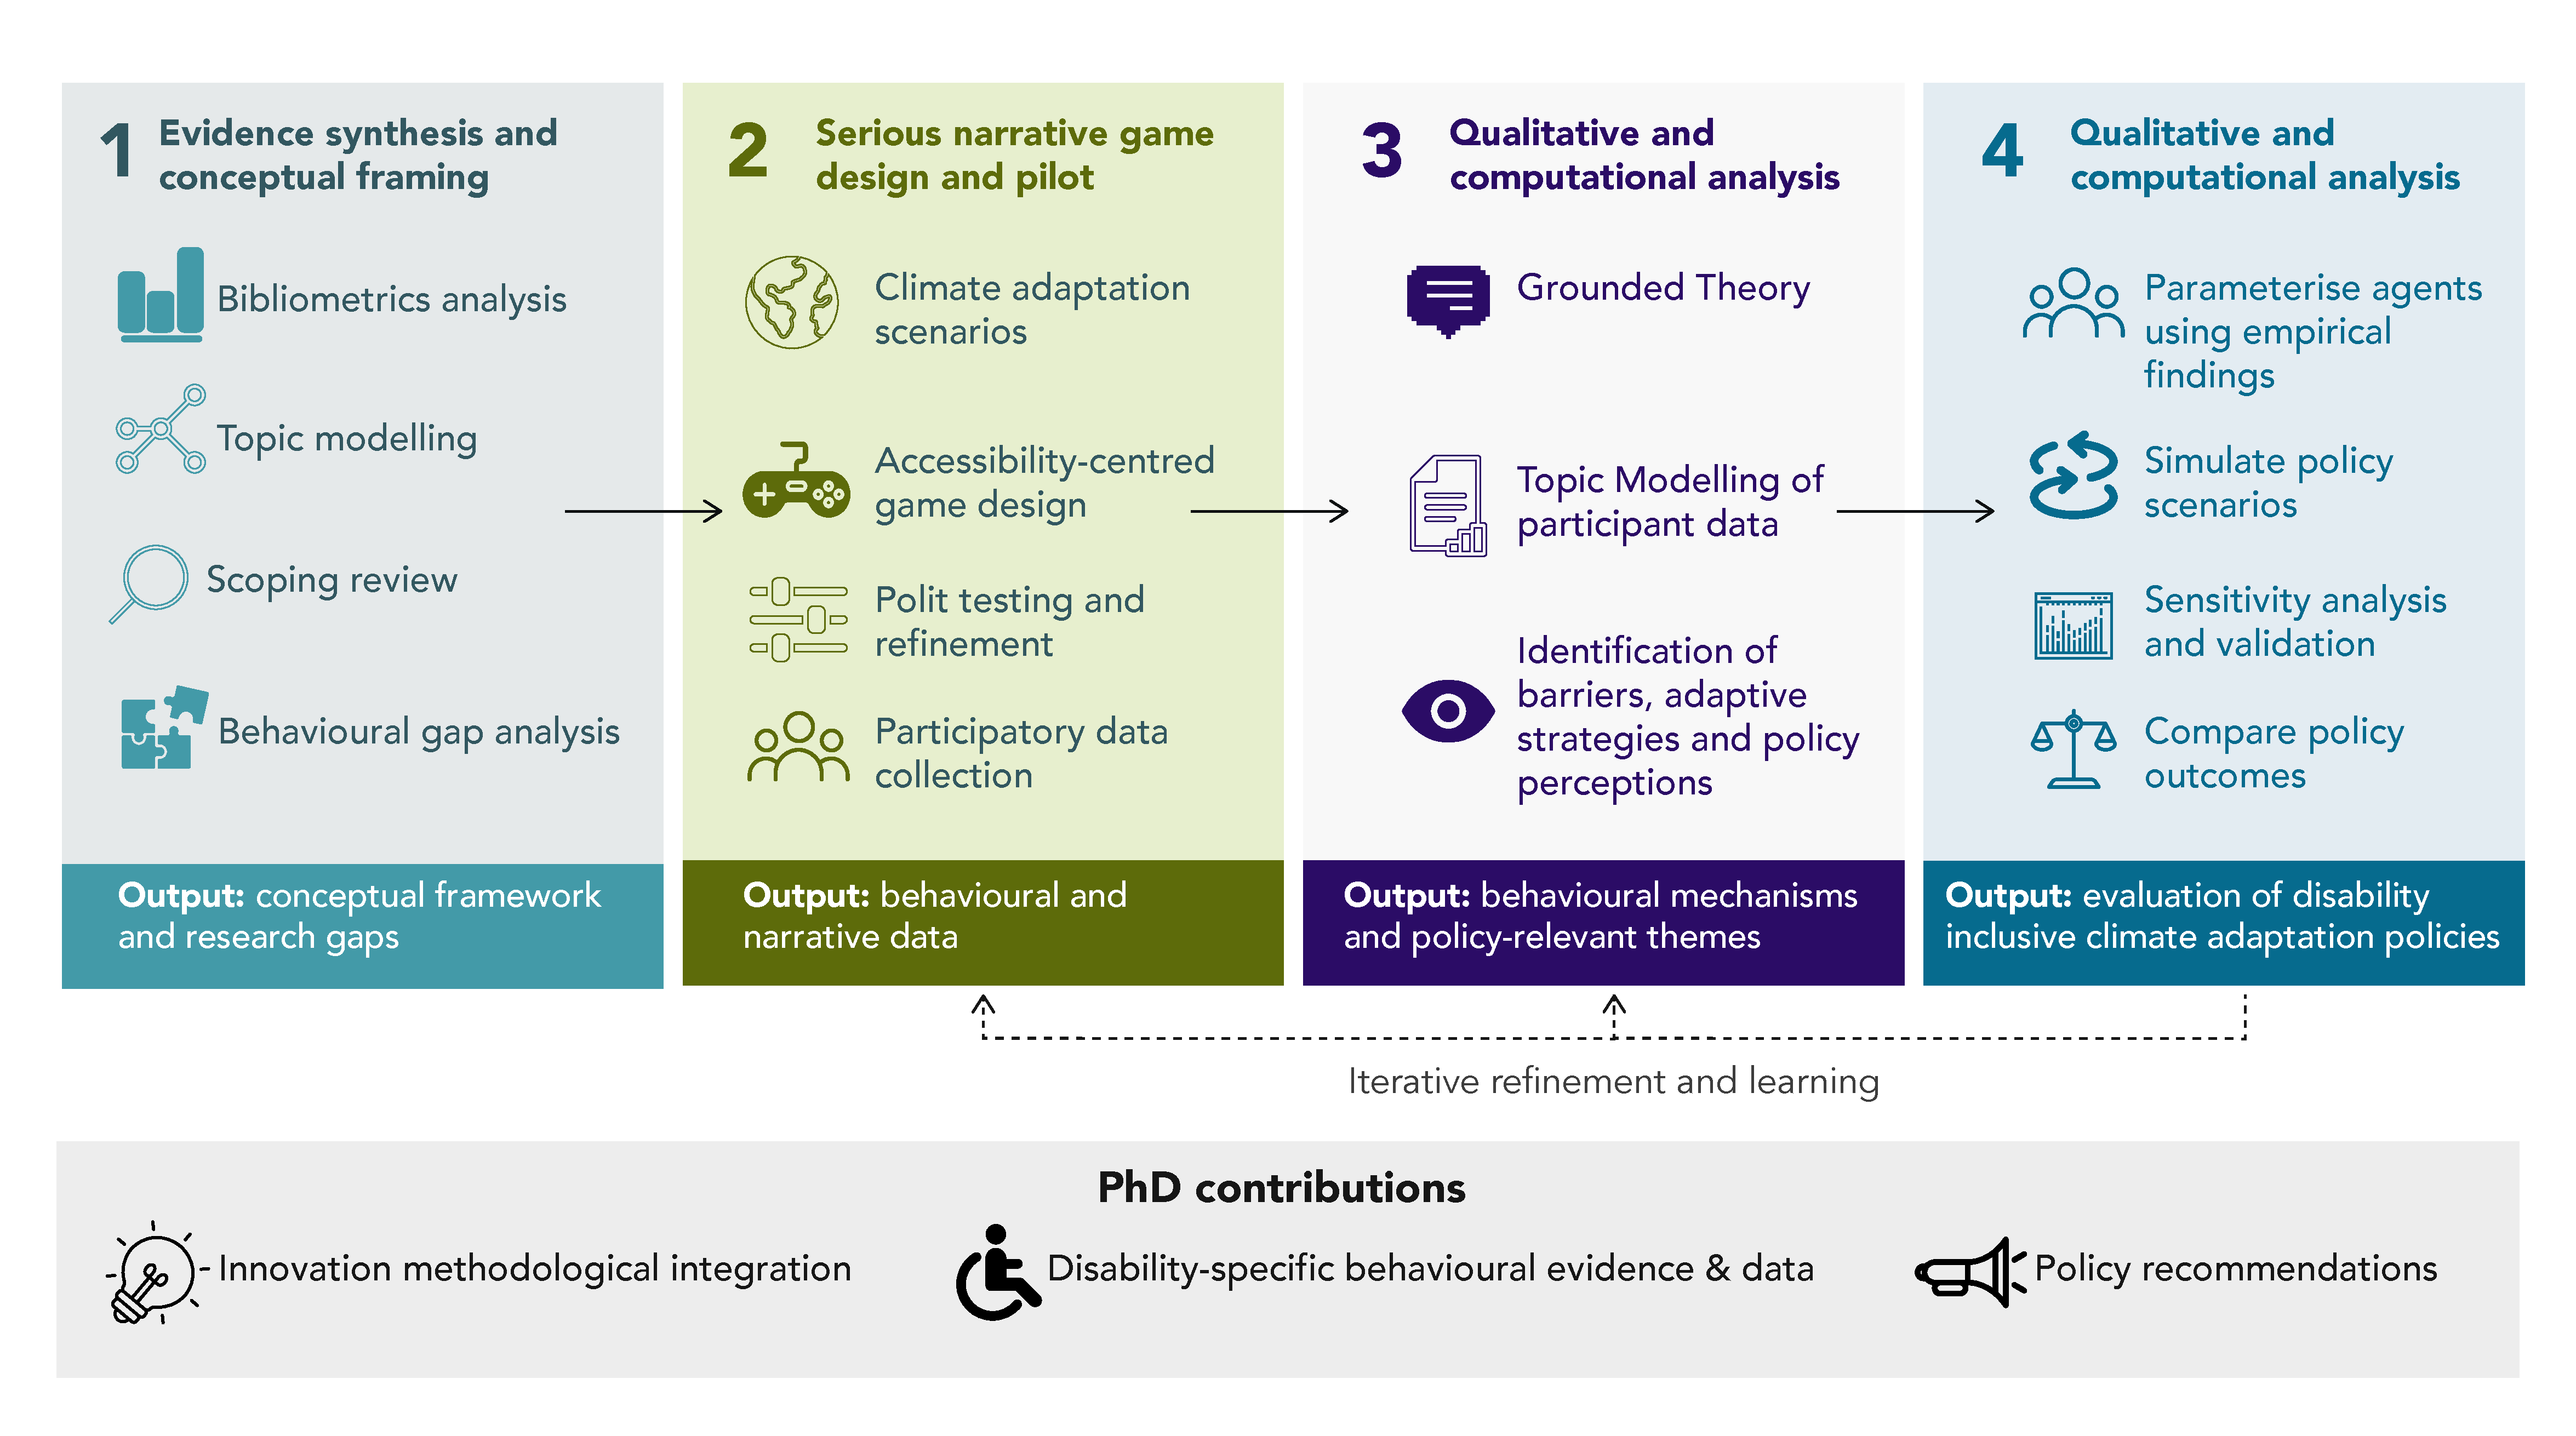
\includegraphics[width=1\linewidth]{Overview 0529.pdf}
    \caption{High-level overview of the four-phase PhD research design.}
    \label{fig:research-overview}
\end{figure}

\section{Structure of the Report}
The report is organised into seven chapters. Chapter~1 introduces the research background, problem, aim, objectives, questions and methodology. Chapter~2 reviews the literature and theoretical foundations. Chapter~3 sets out the conceptual and methodological framework across the four phases. Chapter~4 presents Phase 1, the Year 1 mixed-methods analysis, and identifies the four behavioural patterns and five theoretical frameworks that anchor the rest of the thesis. Chapter~5 presents the preliminary Phase 2 narrative game design and pilot study. Chapter~6 sets out the future research plan for Phases 3 and 4. Chapter~7 concludes the report by summarising Year 1 progress and identifying next steps.
\clearpage

\chapter{Literature and Theoretical Foundations}
\vspace*{-1cm}

This chapter reviews the literature and theoretical foundations of the PhD. It moves from the justice framing of disability and climate change, through the implementation gap in disability-inclusive policy, to the social-behavioural mechanisms that reproduce exclusion. The methodological traditions that the PhD draws on (scenario development and narrative games, GT, TM and ABM) are then developed in Chapter~3.
\clearpage

\section{Disability, Climate Change and Climate Justice}
Disability and climate change is increasingly framed as a justice issue rather than merely one of risk. Persons with disabilities face disproportionate exposure to climate hazards where impairment intersects with disabling social, institutional and environmental conditions: inaccessible infrastructure, limited emergency communication, unequal access to health and transport, and exclusion from decision-making all compound vulnerability \cite{Uddin2024}.

The scale of this concern is considerable. PWDs comprise approximately 16\% of the world's population, an estimated 1.3 billion people \cite{WHO_Global_Report_Health_Equity_Disabilities_2022}, and roughly 80\% live in resource-poor nations where exposure to climate change impacts and disasters is most acute \cite{world2015global}.

Two complementary frameworks help to make sense of this inequity. Disability justice applies across disabilities and centres "access, self-determination, and an expectation of difference" \cite{ortiz2012disability}; it calls for these principles to be embedded within climate and disaster preparedness policies and practices \cite{engelman2022global}. Climate justice, evolving from environmental justice, has broadened from addressing the causes of climate change to confronting the wider inequities it creates or exacerbates \cite{anguelovski2011spatial}  \cite{King2022}, and now concerns the disruption of ecosystems as much as the injustices experienced by vulnerable human communities \cite{schlosberg2014environmental}.

In practice, however, both frameworks remain poorly realised for disabled populations. Many countries have endorsed national and international policies supporting the inclusion of PWDs in climate emergencies and humanitarian settings, yet these commitments often amount to accessibility in name only \cite{engelman2022global}. Disabled people are made vulnerable not by their impairments but by the absence of effective access to information, support and services; discrimination, stigma, social exclusion and economic inequality further amplify their exposure to climate hazards and threaten rights to life, health, water, food, education, livelihood, cultural life, independent living and personal mobility \cite{stein2022disability}. These inequities are deepened by intersections of disability, socioeconomic disadvantage and underlying health conditions, and may even be reproduced by climate mitigation and adaptation strategies that inadvertently introduce new barriers \cite{globaldisabilitysummit2025}. Compounding this, disabled people are less likely to know whom to approach for assistance before, during or after a disaster \cite{palmercase}, while humanitarian responders in developing regions often lack the knowledge, skills and capacity to support them \cite{gartrell2020cambodia}.

Addressing these gaps requires more than recognition. Co-development processes give disabled people greater ownership of emergency response and help to mitigate the effects of disasters \cite{gaskin2017factors}, and meaningful progress depends on participatory approaches that account for the multiple, intersecting vulnerabilities disabled people experience. Advancing climate justice therefore demands accelerated, disability-inclusive climate action \cite{stein2024advancing}; disability-inclusive climate justice solutions are in synergy with universal climate justice goals and benefit entire societies, not just those with disabilities \cite{stein2022disability}.

\section{Disability Rights in Climate Adaptation and Governance}
Empirical research on disability and climate governance has developed primarily within DRR frameworks. The Sendai Framework for DRR (2015--2030) marked a normative shift by explicitly requiring the inclusion of PWDs, and subsequent scholarship has examined how the commitment translates, or fails to translate, into practice \cite{Spurway2016,Lord2025}. The 2015 SDGs reference disability seven times \cite{UNSDGLeaveNoOneBehind}, and the 2016 World Humanitarian Summit Declaration and 2019 IASC Guidelines extend equivalent commitments into humanitarian action \cite{Watts2021LancetCountdown,IASC2019DisabilitiesHumanitarianAction}; the CRPD provides the foundational rights-based instrument across them \cite{UN2006CRPD}. Climate adaptation governance, as distinct from DRR, has been slower to engage with disability: implementation remains weakly monitored and inconsistently reported \cite{Kim2024,Jodoin2020}. The pattern is now theorised as \textit{eco-ableism}, the systematic subordination of disability-related interests within environmental and climate discourse \cite{Harpur2025}, and intersectional analyses extend the diagnosis to show how disability interacts with gender, indigeneity and Global South location to produce compounded exclusion \cite{Murcott2025,Parker2025}. In response, the literature increasingly calls for \textit{participatory justice}: the meaningful involvement of PWDs and DPOs in policy development, priority setting, decision-making and implementation \cite{Polack2008}.

\section{From Vulnerability to Agency and Participation}
A recurring critique concerns the dominance of the vulnerability framing. While documenting disproportionate harm has been politically valuable, treating vulnerability as the defining attribute of disabled populations positions them as objects of protection rather than as participants in the governance arrangements that shape their exposure \cite{stein2022disability,Chukwudum2025}. The literature now documents the specific mechanisms through which disabled people are rendered invisible: framing them as passive recipients rather than as agents within governance processes \cite{Ton2019}, inaccessible communication and the absence of disability data in risk assessments \cite{Grech2025,TannenbaumBaruchi2024}, and institutional fragmentation that constrains disability-inclusive action even where formal commitments exist \cite{Pertiwi2022}.

Two moves in the literature push beyond this framing. The capability approach shifts analytical attention from what disabled people lack to what governance arrangements enable or constrain them to do and to be \cite{Ton2019}, recasting them as agents whose functioning is mediated by the rules, resources and recognition that institutions provide. Participatory and rights-based perspectives extend the move into a procedural one, arguing that meaningful inclusion requires the redesign of governance processes so that disabled people can contribute knowledge, shape priorities and hold institutions accountable \cite{Polack2008}.

\section{Social-Behavioural Mechanisms of Exclusion}
Understanding why disability inclusion fails to translate from policy text into operational practice requires a theoretical account of the social-behavioural mechanisms that reproduce exclusion. Two mid-range social-psychological frameworks are particularly relevant. SDT proposes that societies are organised around group-based hierarchies maintained through behavioural asymmetries, legitimising ideologies and institutional discrimination \cite{sidanius_pratto_1999_socdom}; applied to climate governance, it helps explain the systematic underrepresentation of disabled people as an active process of hierarchy maintenance \cite{King2022}. SJT complements SDT by examining how members of disadvantaged groups may come to endorse and internalise the arrangements that marginalise them \cite{jost_2003_decade}, which illuminates how disabled people may self-exclude from participation \cite{Akike2025}. The two frameworks together provide an analytical vocabulary for examining exclusion as a behavioural and institutional dynamic rather than as a policy failure or resource deficit. The full mapping between mechanisms and theoretical lenses is developed in Section~\ref{sec:mechanisms}.

\section{Summary: Policy Recognition and the Implementation Gap}
The chapter converges on a finding: a persistent implementation gap accompanies the gradual inclusion of disability-inclusive language in international frameworks. The literature is largely biased toward impact assessment and normative advocacy, with relatively little empirical study of the governance mechanisms through which inclusion is implemented or denied \cite{Makuyana2023,Stein2023}. The structural reasons are well documented: the absence of disability data in national risk registers, the limited capacity of disability organisations to participate in technical governance processes, and the marginalisation of disability concerns within climate ministries and adaptation planning bodies \cite{Grossi2023}. From a legal and rights standpoint, policy recognition does not produce implementation pressure because there are no enforced accountability or monitoring structures \cite{Brunne2025}.

The literature reviewed across this chapter therefore shows a field that is normatively developed but empirically thin: the rights-based, climate justice and governance frameworks that frame disability inclusion are well established; the behavioural and institutional mechanisms that produce exclusion are theorised but underspecified empirically; and the methods available to generate participant-driven evidence from disabled people remain limited. No existing study integrates disability behavioural evidence, participatory scenario-based data collection and computational policy simulation into a unified framework for evaluating disability-inclusive climate adaptation. Chapter~3 develops the framework that this PhD proposes in response.

%\subsection{Gap in Existing Literature} The literature reviewed so far suggests several important gaps. First, disability and climate change research has often focused on vulnerability, while paying less attention to agency, participation and leadership. Second, climate adaptation governance literature has recognised inclusion in principle, but has not sufficiently examined how disability-inclusive policies can be evaluated in practice. Third, serious games and scenario-based methods have been used in climate research, but persons with disabilities are rarely central participants or co-designers. Fourth, ABM has strong potential for climate policy simulation, but is rarely calibrated using disability-specific behavioural data.

%This PhD responds to these gaps by integrating four components: a critical review of disability marginalisation in climate governance, a serious narrative game for participatory behavioural data generation, Grounded Theory and Topic Modelling for analysing player responses, and Agent-Based Modelling for evaluating policy equity and effectiveness. 
%A summary of the gap is shown below:

%\begin{table}[htbp]
%\centering
%\footnotesize
%\renewcommand{\arraystretch}{1.25}
%\caption{Summary of literature areas, contributions and limitations}
%\label{tab:literature-areas}

%\begin{tabular}{p{3.1cm} p{5cm} p{5cm}}
%\toprule
%\textbf{Literature area} & \textbf{Main contribution} & \textbf{Key limitation} \\
%\midrule

%Disability and climate justice
%& Establishes rights, vulnerability and justice concerns
%& Limited focus on policy evaluation methods \\

%Disability and disaster governance
%& Shows risk, preparedness and access barriers
%& Often focuses on vulnerability rather than agency \\

%Climate adaptation governance
%& Examines policy design and implementation
%& Disability is often marginal or generalised \\

%Serious games for climate research
%& Supports scenario exploration and engagement
%& Disabled participants are rarely central users \\

%ABM for climate adaptation
%& Simulates complex policy and behavioural scenarios
%& Rarely uses disability-specific behavioural data \\

%GT and Topic Modelling
%& Supports qualitative and computational analysis
%& Rarely integrated with serious games and ABM in this field \\

%\bottomrule
%\end{tabular}
%\end{table}
%\subsection{Summary}
%Overall, the literature shows that disability inclusion in climate adaptation remains an underdeveloped area, particularly in relation to participation, behavioural evidence and policy evaluation. Existing research has established that persons with disabilities face disproportionate climate risks, but less is known about how they respond to adaptation policies or how their experiences can be translated into policy simulation.

%This chapter therefore provides the foundation for the proposed PhD framework. The next chapter develops this framework by linking the Year 1 review, serious narrative game design, Grounded Theory, Topic Modelling and Agent-Based Modelling into a coherent research design for evaluating disability-inclusive climate adaptation policies.

%Climate change heightens multidimensional inequalities and intensifies issues like water scarcity, hunger, and poverty\cite{stein2022disability},\cite{gaskin2017factors}, disproportionately affecting marginalized groups, particularly people with disabilities (PWDs). They have a disaster mortality rate up to four times higher than people without disabilities, along with increased injury risk and abandonment.  PWDs face higher mortality, poorer health, and more challenges during emergencies, worsened by climate change\cite{kosanic2022inclusive}. The vulnerability of PWDs to climate change is well-recognized. From the adoption of the Convention on the Rights of Persons with Disabilities in 2006, which established disability as a rights-based and participatory domain, to the explicit recognition of persons with disabilities within global climate governance under the Paris Agreement (2015) and the Sendai Framework for Disaster Risk Reduction (2015), international policy has gradually—but unevenly—asserted the inclusion of persons with disabilities in climate action. Subsequent instruments, including UN Human Rights Council resolutions on human rights and climate change (2019; 2021) and interpretative work by the Office of the High Commissioner for Human Rights, have further articulated the need for disability-inclusive approaches to climate adaptation and response, while recent statements by the CRPD Committee (2024) emphasise participation and agency within climate and disaster governance. However, internationally, there is no disability constituency in the UN Framework Convention on Climate Change, in contrast to the constituencies that exist for Indigenous people, women and gender, and youth. Despite growing research, no global policy fully addresses PWDs' needs\cite{madans2017measuring}, and most focus on their vulnerabilities over adaptive capacities\cite{3}. Frameworks like the 2030 Agenda, CRPD and UNFCCC\cite{UNISDR_Sendai_Framework_2015} emphasize inclusion in climate action\cite{UN_CRPD_2006}, but implementation is limited, PWDs are excluded from decision-making processes\cite{UN_Paris_Agreement_2015}. Many governments lack preparedness\cite{gaskin2017factors}, only 5 per cent of parties addressed PWDs in a 2023 report. As a result, 86 per cent of PWDs are excluded from risk reduction decisions, and 84 per cent lack disaster plans\cite{UN_Disability_Development_Report_2024},\cite{gaskin2017factors,eriksen2021crdps}. PWDs have low involvement in policy development, decision-making, and implementation\cite{stein2022disability}. There is also a significant research gap on the intersection of disability and climate change\cite{Jones_Disability_Inclusive_Climate_2023}, particularly in gathering comprehensive data and understanding how advocacy shapes policymakers' views\cite{4,debnath2023facilitating}. This is primarily due to exclusion from inclusive planning, accessible information, and health services. PWDs represent 16 per cent of the global population\cite{kosanic2022inclusive}, and over 1 billion of them have significant disability. 

%Addressing these challenges requires participatory justice, aligning with the UN Sustainable Development Goals and Convention on the Rights of Persons with Disabilities (CRPD) Obligations\cite{stein2022climate}. Therefore, systematic research, combining qualitative and quantitative methods, is essential\cite{alcamo2001scenarios,alcamo2008environmental}. Scenario development is a valuable tool for integrated assessments, sustainability science, and public policy planning, as it integrates knowledge and human choices to explore complex and uncertain future options\cite{van2008new}. In climate policy research, this approach includes modelling and narrative to inform decisions\cite{rounsevell2010developing}.
\clearpage

\chapter{Methodological Framework Design}
\vspace*{-1cm}

This chapter sets out the four-phase methodological framework of the PhD. Phase 1 is a mixed-methods scoping review combining bibliometric analysis, TM and qualitative synthesis. Phases 2 and 3 design and pilot a narrative game and analyse the data it generates. Phase 4 uses ABM to simulate the performance of disability-inclusive policies under behavioural heterogeneity, moving the analysis from diagnosis of exclusion to policy evaluation.
\clearpage

\section{Framework Overview}
The PhD addresses a problem that is simultaneously conceptual and methodological. The gap between commitments to disability-inclusive climate policy and their implementation cannot be explained by normative deficits alone; what is missing is a theoretically grounded account of the behavioural and institutional mechanisms that reproduce exclusion, together with an empirical method capable of generating evidence from disabled people as active agents in governance rather than as subjects of risk assessment. The framework integrates four interconnected phases organised around three core concepts: \textit{exclusion mechanisms}, the structural and behavioural processes by which disabled people are marginalised in climate adaptation governance; \textit{adaptive behaviour}, the decision-making strategies and policy responses they enact under climate stress; and \textit{policy evaluation}, the simulation of disability-inclusive adaptation policy scenarios under social complexity.

\section{Overall Research Design}
The framework follows a staged analytical logic in which each phase produces a distinct kind of knowledge that enables the next. 
 \begin{itemize}
\item Phase 1 produces mapping knowledge: a systematic understanding of how disability has been conceptualised in the literature, where the behavioural evidence base is thin, and what exclusion mechanisms existing research identifies. 
 \end{itemize}
 \begin{itemize}
\item Phase 2 produces behavioural knowledge: participant-generated data on how disabled people navigate climate adaptation scenarios. 
 \end{itemize}
  \begin{itemize}
\item Phase 3 develops categorical knowledge: empirically grounded theoretical categories derived from game data through GT and TM. 
\end{itemize}
  \begin{itemize}
\item Phase 4 generates simulation knowledge: ABMs populated with these categories to test policy scenarios under dynamic social conditions.
\end{itemize}
The progression is cumulative rather than modular: the game cannot be designed without the conceptual and evidential grounding from Phase 1, and the ABM cannot be populated without the behavioural categories from Phase 3. As indicated in Figure~\ref{fig:phase1-4-framework}, the framework is also iterative, with findings from later phases prompting refinement of earlier assumptions. The overall stance is critical realist: Governance structures and mechanisms of exclusion are real and have an impact on outcomes whether we see them or not, but can only be studied through what people think, speak, and act, and that is why the PhD brings together qualitative, design, computational and participatory methods.

\begin{figure}[H]
    \centering
    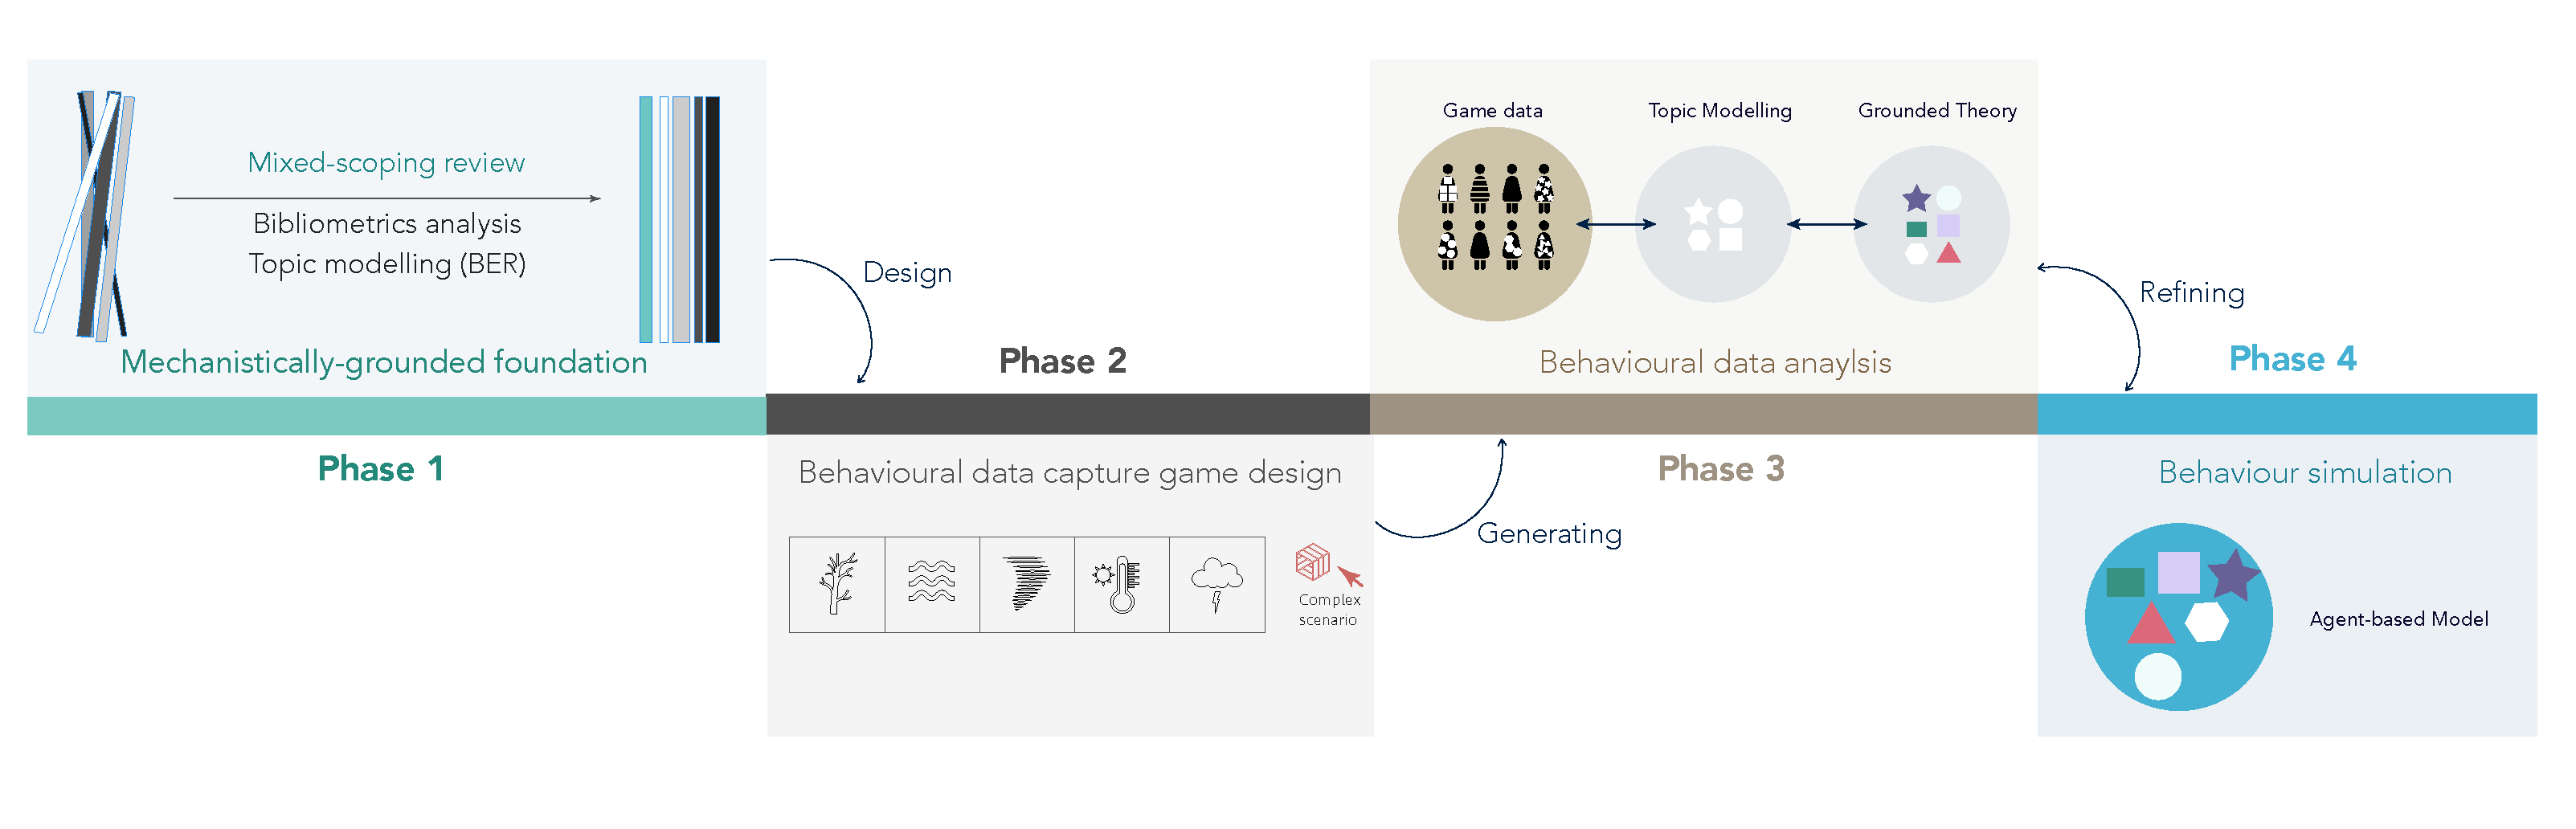
\includegraphics[width=1\linewidth]{Phase 1-4.pdf}
    \caption{Detailed four-phase methodological framework, showing the analytical workflow and feedback loops from Phase 1 through Phase 4.}
    \label{fig:phase1-4-framework}
\end{figure}



The four phases are operationalised in the chapters that follow. Phase~1, a mixed-methods scoping review combining bibliometric analysis, TM and qualitative synthesis across the 267-record extended and 42-record core datasets, is reported in Chapter~4 and yields the conceptual framework of exclusion mechanisms and the design parameters for the game. Phase~2 translates those parameters into the narrative game developed in Chapter~5. Phases~3 and~4, set out in Chapter~6, analyse the resulting data through GT and TM and translate the behavioural categories into the ABM that simulates how disability-inclusive adaptation policies perform under heterogeneity. Each phase thus supplies the input the next requires, carrying the analysis from literature-based gap diagnosis through to computational policy evaluation.




%\begin{figure}[H]
  %  \centering
   % 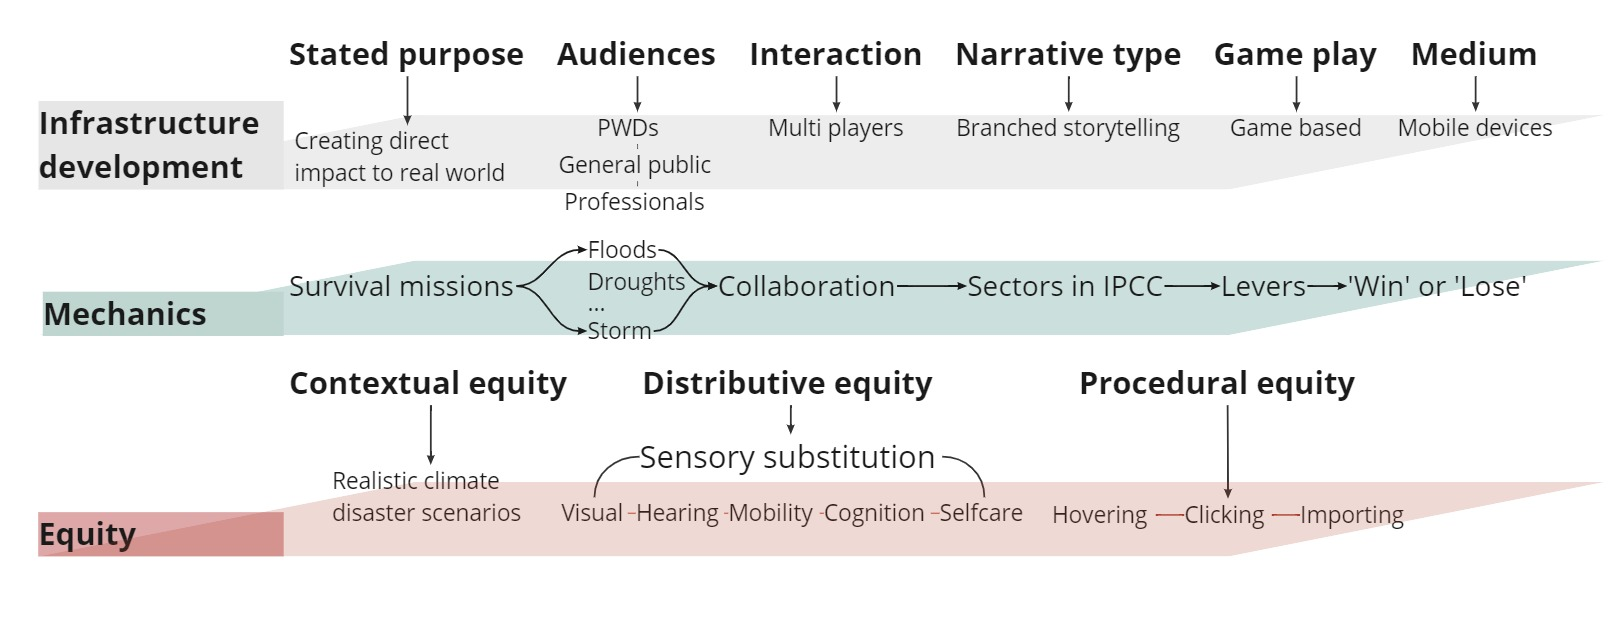
\includegraphics[width=1\linewidth]{Game2.jpg}
  %  \caption{Three-layer framework for serious narrative game design.}
  %  \label{fig:enter-label}
%\end{figure}


\clearpage

\chapter{Phase 1 — Year 1 Mixed-Methods Analysis}
\vspace*{-1cm}

\noindent\textbf{Background}: Disability is increasingly recognised in climate adaptation and disaster governance policy, yet recognition rarely translates into operational practice. The literature documenting this gap is fragmented across disability studies, disaster risk reduction and climate justice, and lacks a unified account of the mechanisms through which exclusion is reproduced.

\noindent\textbf{Aim}: This chapter reports the Phase 1 work of the PhD, a mixed-methods scoping review that maps how persons with disabilities are positioned in the climate adaptation and disaster governance literature, and derives a set of social-behavioural mechanisms that explain why exclusion persists and that can inform the participatory and computational phases that follow.

\noindent\textbf{Method}: Three analytical methods are combined: a bibliometric and keyword co-occurrence analysis of a 267-record extended dataset; a BERTopic TM analysis of the same dataset; and a qualitative synthesis of a 42-record core dataset selected through PRISMA screening.

\noindent\textbf{Result}: The three analyses identify four recurrent behavioural patterns (vulnerability framing, internalised acceptance of token inclusion, DPO led participation, and institutional normalisation) and five social-science frameworks that account for them. The chapter closes by translating these findings into the design criteria that guide the empirical phases developed in Chapters~5 and~6.

\vspace{0.3cm}
\noindent\textbf{Keywords:} scoping review; bibliometric analysis; topic modelling; qualitative synthesis; disability; climate governance; exclusion mechanism.

\clearpage
\section{Introduction}
Disability has long presented multidimensional barriers to inclusion and participation in decision-making, restricting access to education, health services, employment and the information and economic security that follow from them \cite{trani2018realization}. Climate change compounds health inequalities, yet adaptation policy routinely fails to consider disability-inclusive measures \cite{wilbur2025climate}.

Chapter~2 has shown that disability is increasingly recognised within the climate adaptation, DRR and climate justice literatures, but that this recognition has yet to translate into meaningful implementation. The same pattern is visible in the principal international instruments: major frameworks such as the Nationally Determined Contributions (NDCs) under the Paris Agreement and the 2030 SDGs often fail to address PWDs despite their heightened vulnerability \cite{evmorfidis2026climate}; of the 195 parties to the Paris Agreement, only 41 mention PWDs in their active NDCs and only 17 include concrete inclusion measures, while just six refer explicitly to disability rights and five recognise the importance of integrating disabled people's knowledge into climate decision-making \cite{jodoin2025systematic,cabo_verde_ndc_2021,maldives_ndc_2020,vietnam_ndc_2022}.

Despite this growing visibility, the existing literature remains fragmented across disability studies, disaster risk reduction and climate justice, and lacks a unified account of the social-behavioural mechanisms through which exclusion is reproduced. Behavioural evidence generated with disabled people themselves is thin, participation is largely framed as consultation rather than as agency, and policy-relevant evaluation of disability-inclusive adaptation interventions is rare. It is this conceptual, evidential and methodological gap that Phase 1 sets out to map.

%\subsection{Aim and Review Questions}

% More specifically, the review has four objectives:
% \begin{itemize}
%     \item To map the overall structure and thematic distribution of the disability–climate governance literature.
% \end{itemize}
% \begin{itemize}
%     \item To identify how persons with disabilities are conceptualised and positioned within existing research, particularly in relation to vulnerability, participation, adaptation and governance.
% \end{itemize}    
% \begin{itemize}
%     \item To examine the structural, institutional and social-behavioural mechanisms through which disability marginalisation is reproduced within climate governance systems.
% \end{itemize}    
% \begin{itemize}
%     \item To develop the behavioural foundation for the implementation of disability-inclusive climate adaptation policies.
% \end{itemize} 

% The review is guided by the following review questions:

% \begin{itemize}
%     \item How are persons with disabilities conceptualised and positioned within climate adaptation, disaster governance and climate justice literature?
%     \end{itemize}
% \begin{itemize}
%     \item What dominant thematic patterns, research clusters and knowledge structures characterise the field?
%     \end{itemize}
% \begin{itemize}
%     \item What structural, institutional and social-behavioural mechanisms contribute to the marginalisation of persons with disabilities in climate governance?
%     \end{itemize}
% What conceptual, methodological and evidential gaps remain within the existing literature, particularly in relation to behavioural evidence, participation and policy evaluation?
\section{Research methods and design}
\subsection{Approach}

Phase 1 adopts an integrated review approach that combines bibliometric analysis, TM and qualitative synthesis, on the principle that quantitative and qualitative evaluation are complementary and that their combination produces more replicable and methodologically transparent reviews than qualitative work alone \cite{shen_lai_2022_souvenirs,hicks_2015_leiden_manifesto}. Bibliometric analysis is the systematic, quantitative study of scientific literature through author, citation and keyword analysis, used to identify patterns, trends and impact within a research area \cite{passas2024bibliometric,ragazou2022investigating}. TM is a statistical technique for extracting latent thematic structures from large text corpora \cite{blei2012probabilistic,barde2017overview,ogunleye_2025_topic}. Qualitative synthesis then operates on a narrower, conceptually focused subset to support close interpretation of how concepts are framed and where gaps lie; the capability approach and critical disability studies anchor this synthesis, with SDT and SJT used as supplementary lenses where the empirical patterns match them.

This integrated approach is implemented within a scoping review framework. A scoping review is a form of knowledge synthesis that maps the extent, range and nature of evidence on a broad or emerging topic, clarifies key concepts and identifies gaps in the literature, rather than appraising and pooling findings to answer a narrowly defined question as a systematic review does \cite{arksey2005scoping,levac2010scoping,munn2018systematic}. It is the appropriate methodology for the present research because the literature at the intersection of disability and climate governance is fragmented and conceptually unsettled, and because the objective of Phase~1 is to map how disabled people are positioned and where behavioural evidence is thin, surfacing the conceptual framings and structural gaps that inform the later design stages, rather than to estimate the effect of a defined intervention \cite{munn2018systematic}.

The sequencing is rigorous in its logic: because the disability and climate change literature is fragmented and conceptually unclear, beginning directly with qualitative synthesis would risk making selection and interpretation overly dependent on the researcher's prior assumptions. The analysis is therefore organised around two datasets (Figure~4.1). The 267-record extended dataset supports bibliometric analysis and TM, providing publication, journal, citation, geographical and thematic mapping across the wider literature. The 42-record core dataset supports the qualitative synthesis of conceptual framing, exclusion mechanisms and the positioning of PWDs in climate governance research. The primary output of Phase~1 is a conceptual framework of exclusion mechanisms and a set of design parameters for the narrative game in Phase~2.


\begin{figure}[H]
    \centering
    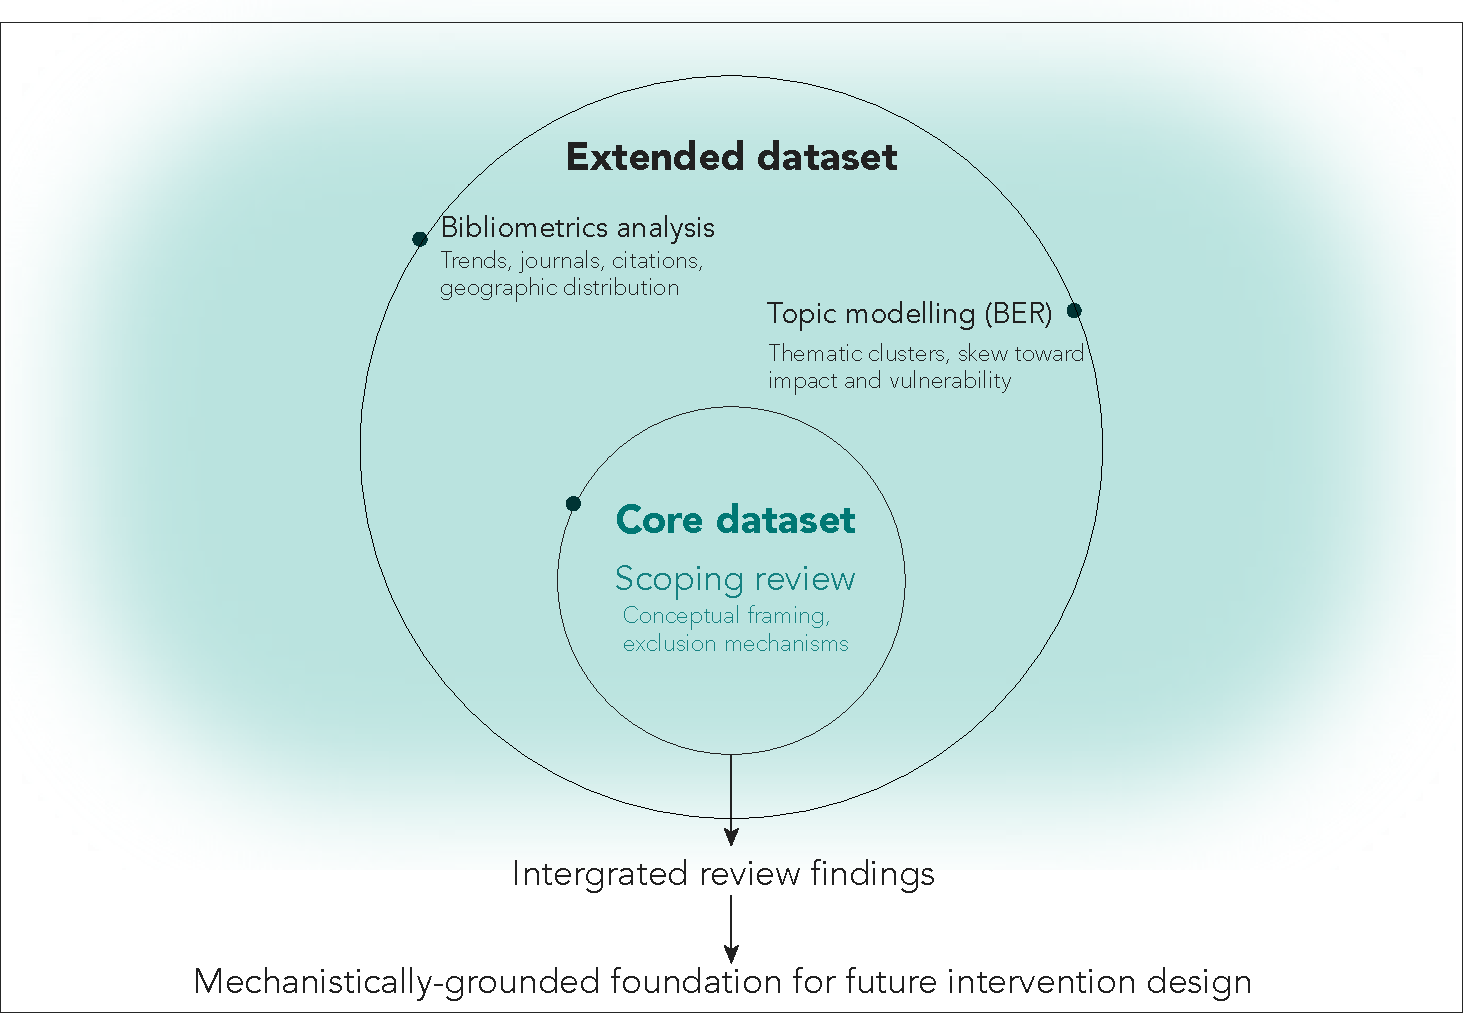
\includegraphics[width=0.8\linewidth]{Asset 7_1.pdf}
    \caption{Overall methodological framework of the phase 1 review}
    \label{fig:enter-label}
\end{figure}

\subsection{Review Data Collection}
Literature searches were conducted in Web of Science, Scopus and PubMed to identify literature at the intersection of disability and climate governance. These three databases were chosen for their complementary coverage: Web of Science and Scopus provide broad multidisciplinary indexing of social science, policy and environmental research, while PubMed adds depth in the health and disability literature. The search strategy consisted of two sets of keywords: those related to climate governance and those related to disability/accessibility. The disability-related terms were informed by the WHO International Classification of Functioning, Disability and Health (ICF) \cite{who_2001_icf} that conceptualises disability as impairments, activity limitations and participation restrictions and understands functioning and disability as an outcome of interactions between health conditions and contextual factors. We have used this framework because it corresponds to how disability is often operationalised across climate, health, disaster risk and governance research. The complete search string and the full list of keywords are provided in Appendix A.

In the exploratory phase, we tested vulnerability-related terms like “vulnerabl*”, but removed them from the final search, as they expanded the results to 70,687 records and mostly captured broad climate vulnerability studies where disability was only marginally mentioned. In doing so, disability remained a distinct analytical category rather than simply another label of common vulnerability.
The search was restricted to records published between 2006 and 2025. The 2006 start date corresponds to the adoption of the CRPD, which marks the point at which disability inclusion became a formal international policy commitment relevant to climate and disaster governance \cite{UN_CRPD_2006}; 2025 reflects the end of the Year~1 search window.

The review followed the methodological framework for scoping studies proposed by Arksey and O'Malley and refined by Levac et al. \cite{arksey2005scoping,levac2010scoping}, and is reported in accordance with the PRISMA extension for Scoping Reviews (PRISMA-ScR) \cite{tricco2018prisma}. Records were imported into Rayyan for screening. The identification, screening and inclusion of relevant literature are summarised in the PRISMA-ScR flow diagram (Figure~\ref{fig:prisma-flow}). Following screening, 267 papers were retained as the extended dataset.

A dual dataset structure was then applied. The full extended dataset of 267 papers supported the bibliometric analysis and topic modelling, while a core dataset of 42 papers was selected from these records through a further eligibility stage for in-depth qualitative synthesis. This strategy allowed the review to combine broad quantitative mapping across the wider literature with deeper qualitative interpretation through social-behavioural lenses.

\begin{figure}[H]
    \centering
    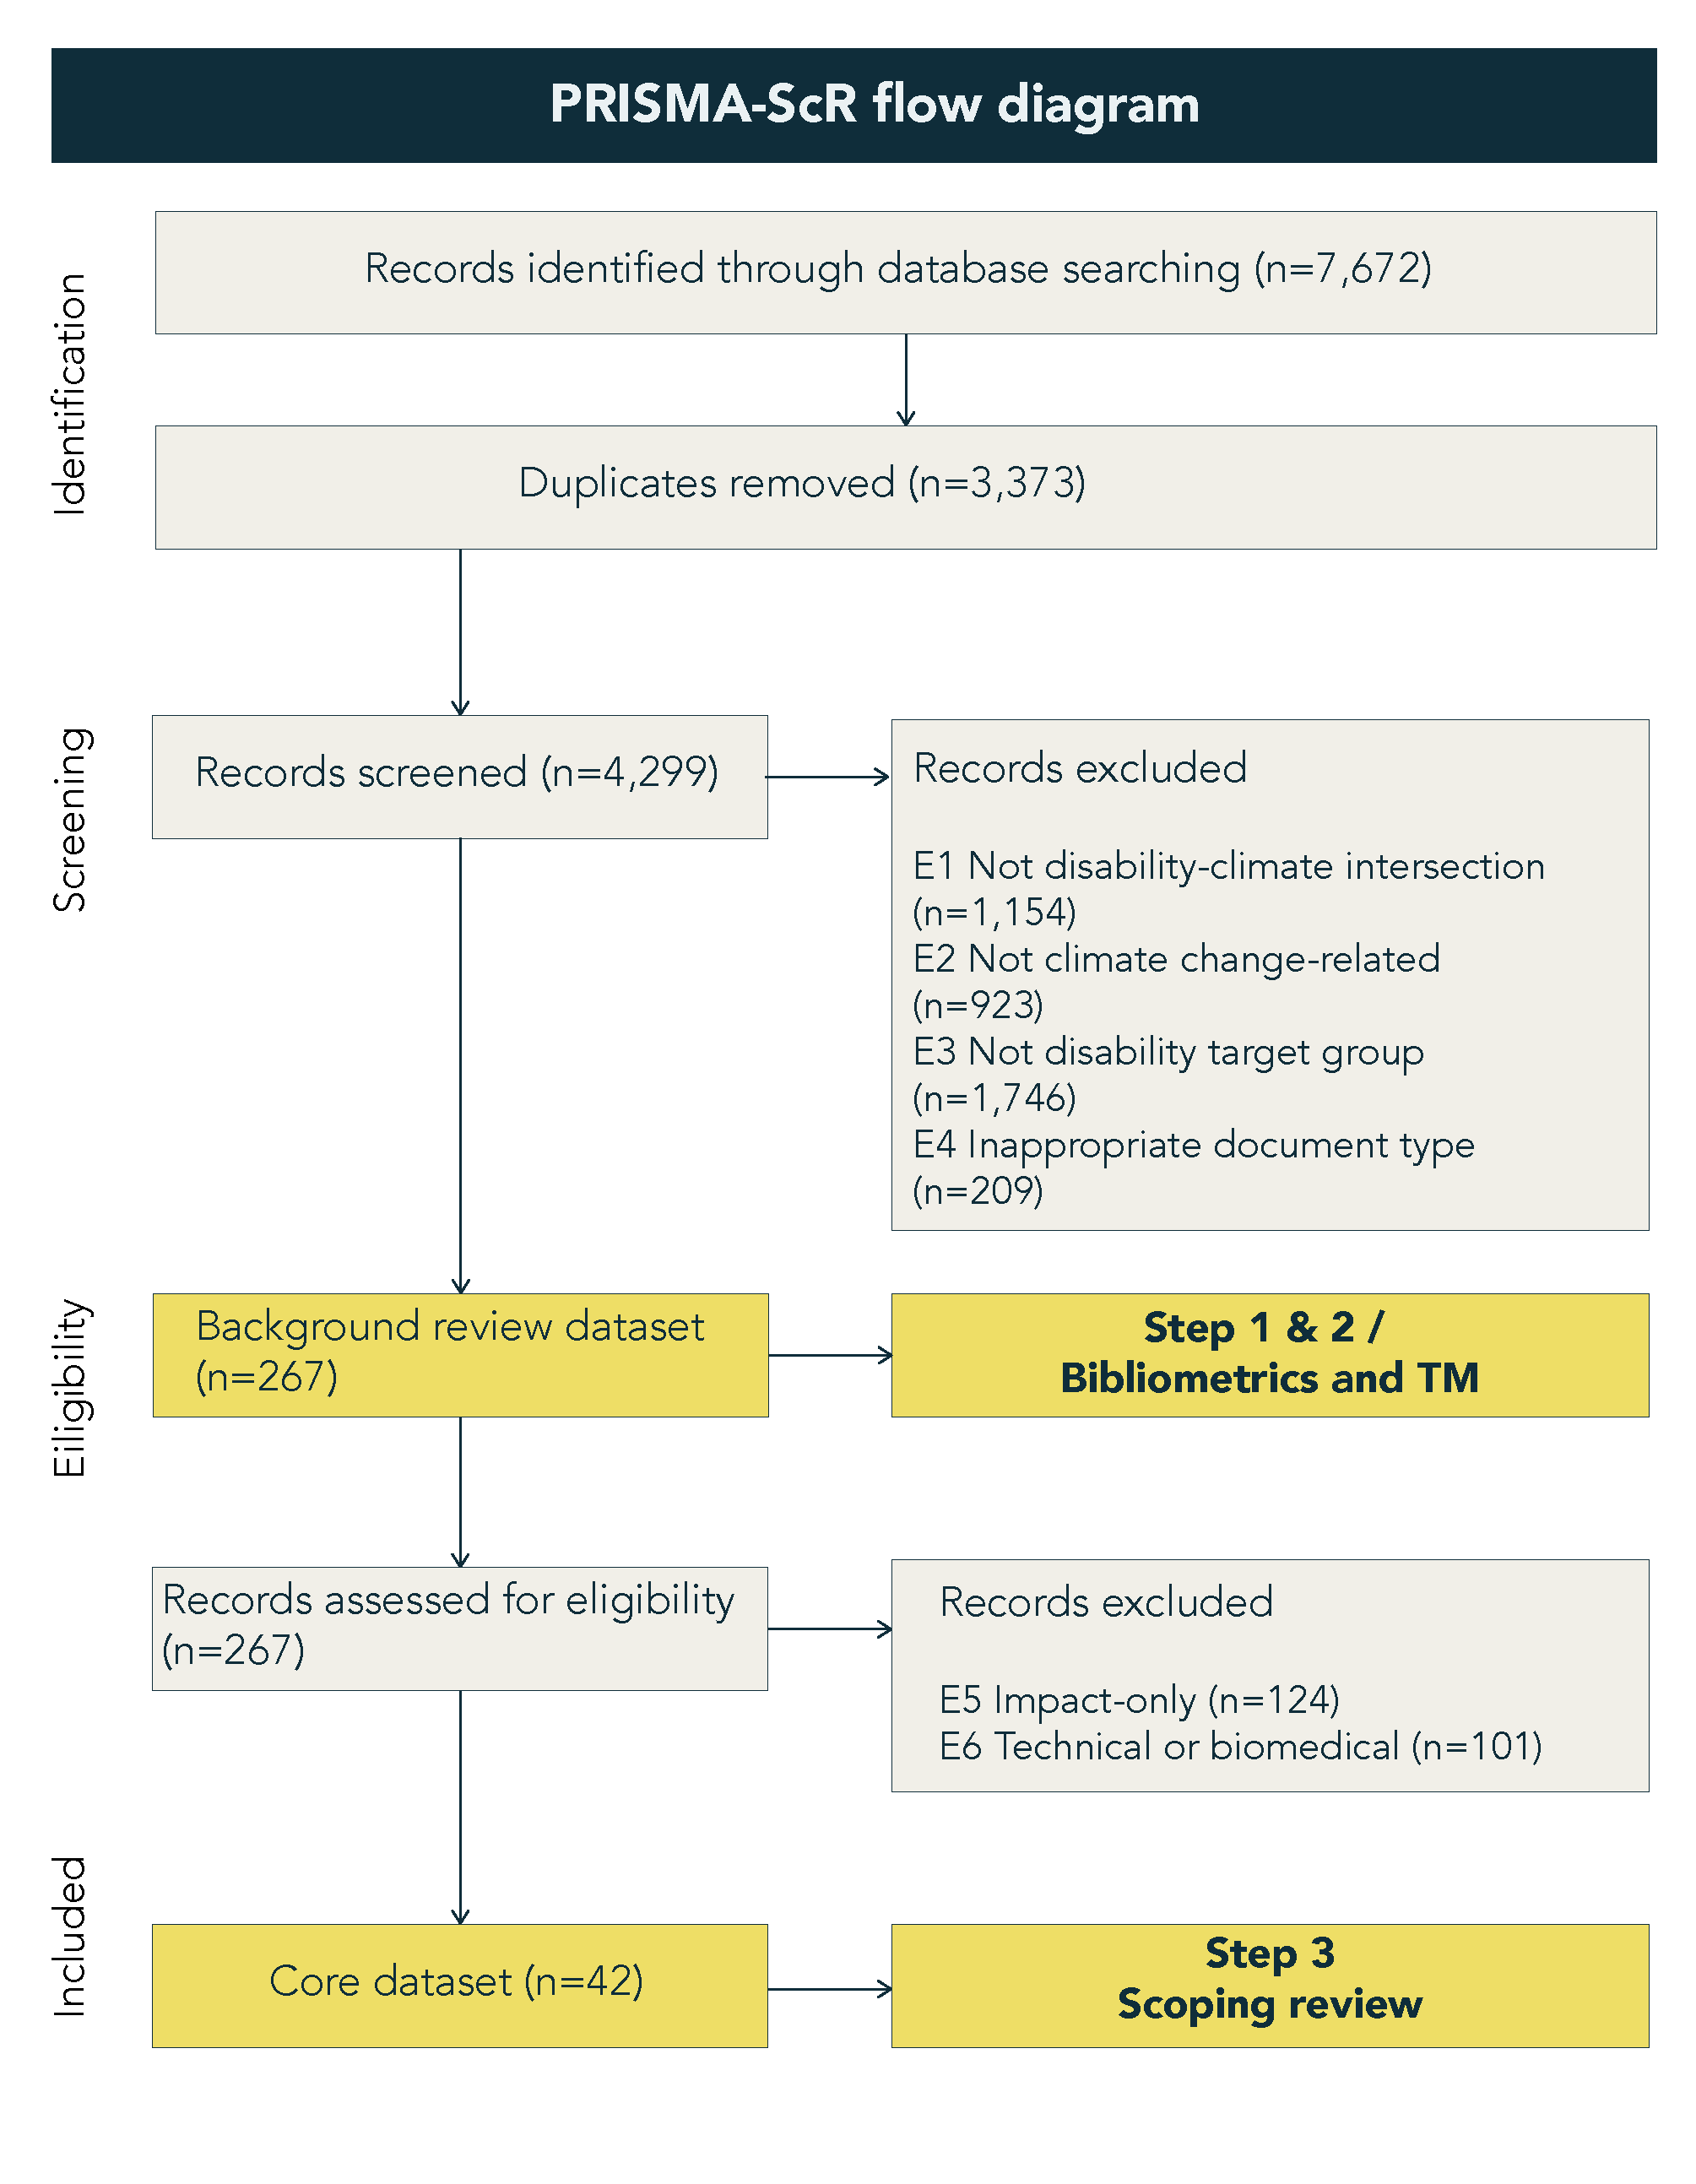
\includegraphics[width=0.7\linewidth]{Prisma.pdf}
    \caption{PRISMA flow diagram of the literature search and screening process (2006--2025).}
    \label{fig:prisma-flow}
\end{figure}

\section{Bibliometric procedure}
Bibliometric analysis was conducted on the extended dataset to map the structure, development and thematic organisation of research on disability and climate governance, using publication trends, keyword co-occurrence, citation structures and geographical distribution. The methods are well suited to reviewing fragmented research fields because they offer a systematic and replicable way to examine the intellectual, social and conceptual structure of a literature \cite{zupic_cater_2015_bibliometric,donthu_2021_bibliometric,linnenluecke_2020_systematic}.

Two complementary software tools were used. VOSviewer is well suited to constructing keyword co-occurrence maps and to identifying thematic clusters and temporal patterns through overlay visualisation \cite{van_eck_waltman_2010_vosviewer,van_eck_waltman_2014_visualizing}. Gephi adds quantitative network analysis and modularity-based community detection, producing structural metrics—graph density, weighted degree, clustering coefficient and centrality—and an alternative community partition that complements the VOSviewer clusters \cite{newman_2006_modularity}. Used together, they allow the conceptual structure of the literature to be read both as a topical map (VOSviewer) and as a quantified network of interconnections (Gephi). 


\subsection{Keyword co-occurrence matrix -- VOSviewer}
Keyword co-occurrence is a standard bibliometric tool for identifying conceptual relationships and the intellectual structure of a research field \cite{zupic_cater_2015_bibliometric,donthu_2021_bibliometric}: nodes represent keywords, edges represent co-occurrence within the same records, and a denser network indicates a more integrated conceptual vocabulary.

Co-occurrence analysis was performed on all author and indexed keywords using VOSviewer. To improve the quality of the analysis, a thesaurus file was applied to merge spelling and abbreviation variants and to remove non-substantive terms generated by the database index (such as \textit{human}, \textit{article}, \textit{review}). The minimum occurrence threshold was set to 5, leaving 51 keywords for analysis. The resulting map (Figure 4.3) groups these terms into 6 thematic clusters, with 511 links and a total link strength of 1{,}513, indicating a dense and unevenly distributed pattern of co-occurrence rather than isolated topical pockets.

Climate change, disability and persons with disabilities are the dominant nodes and are strongly connected with disasters, vulnerability, disaster preparedness, disaster risk reduction, risk assessment, public health, environmental justice, sustainable development and adaptation. The map also reveals an imbalance: risk- and disaster-related terms are more central and densely connected than terms related to participation, decision-making, policy, human rights, climate justice and disability inclusion. Existing research has therefore made substantial progress on the disproportionate risks faced by PWDs, but considerably less on how disabled people participate in, respond to or shape climate adaptation policies.

\begin{figure}[H]
    \centering
    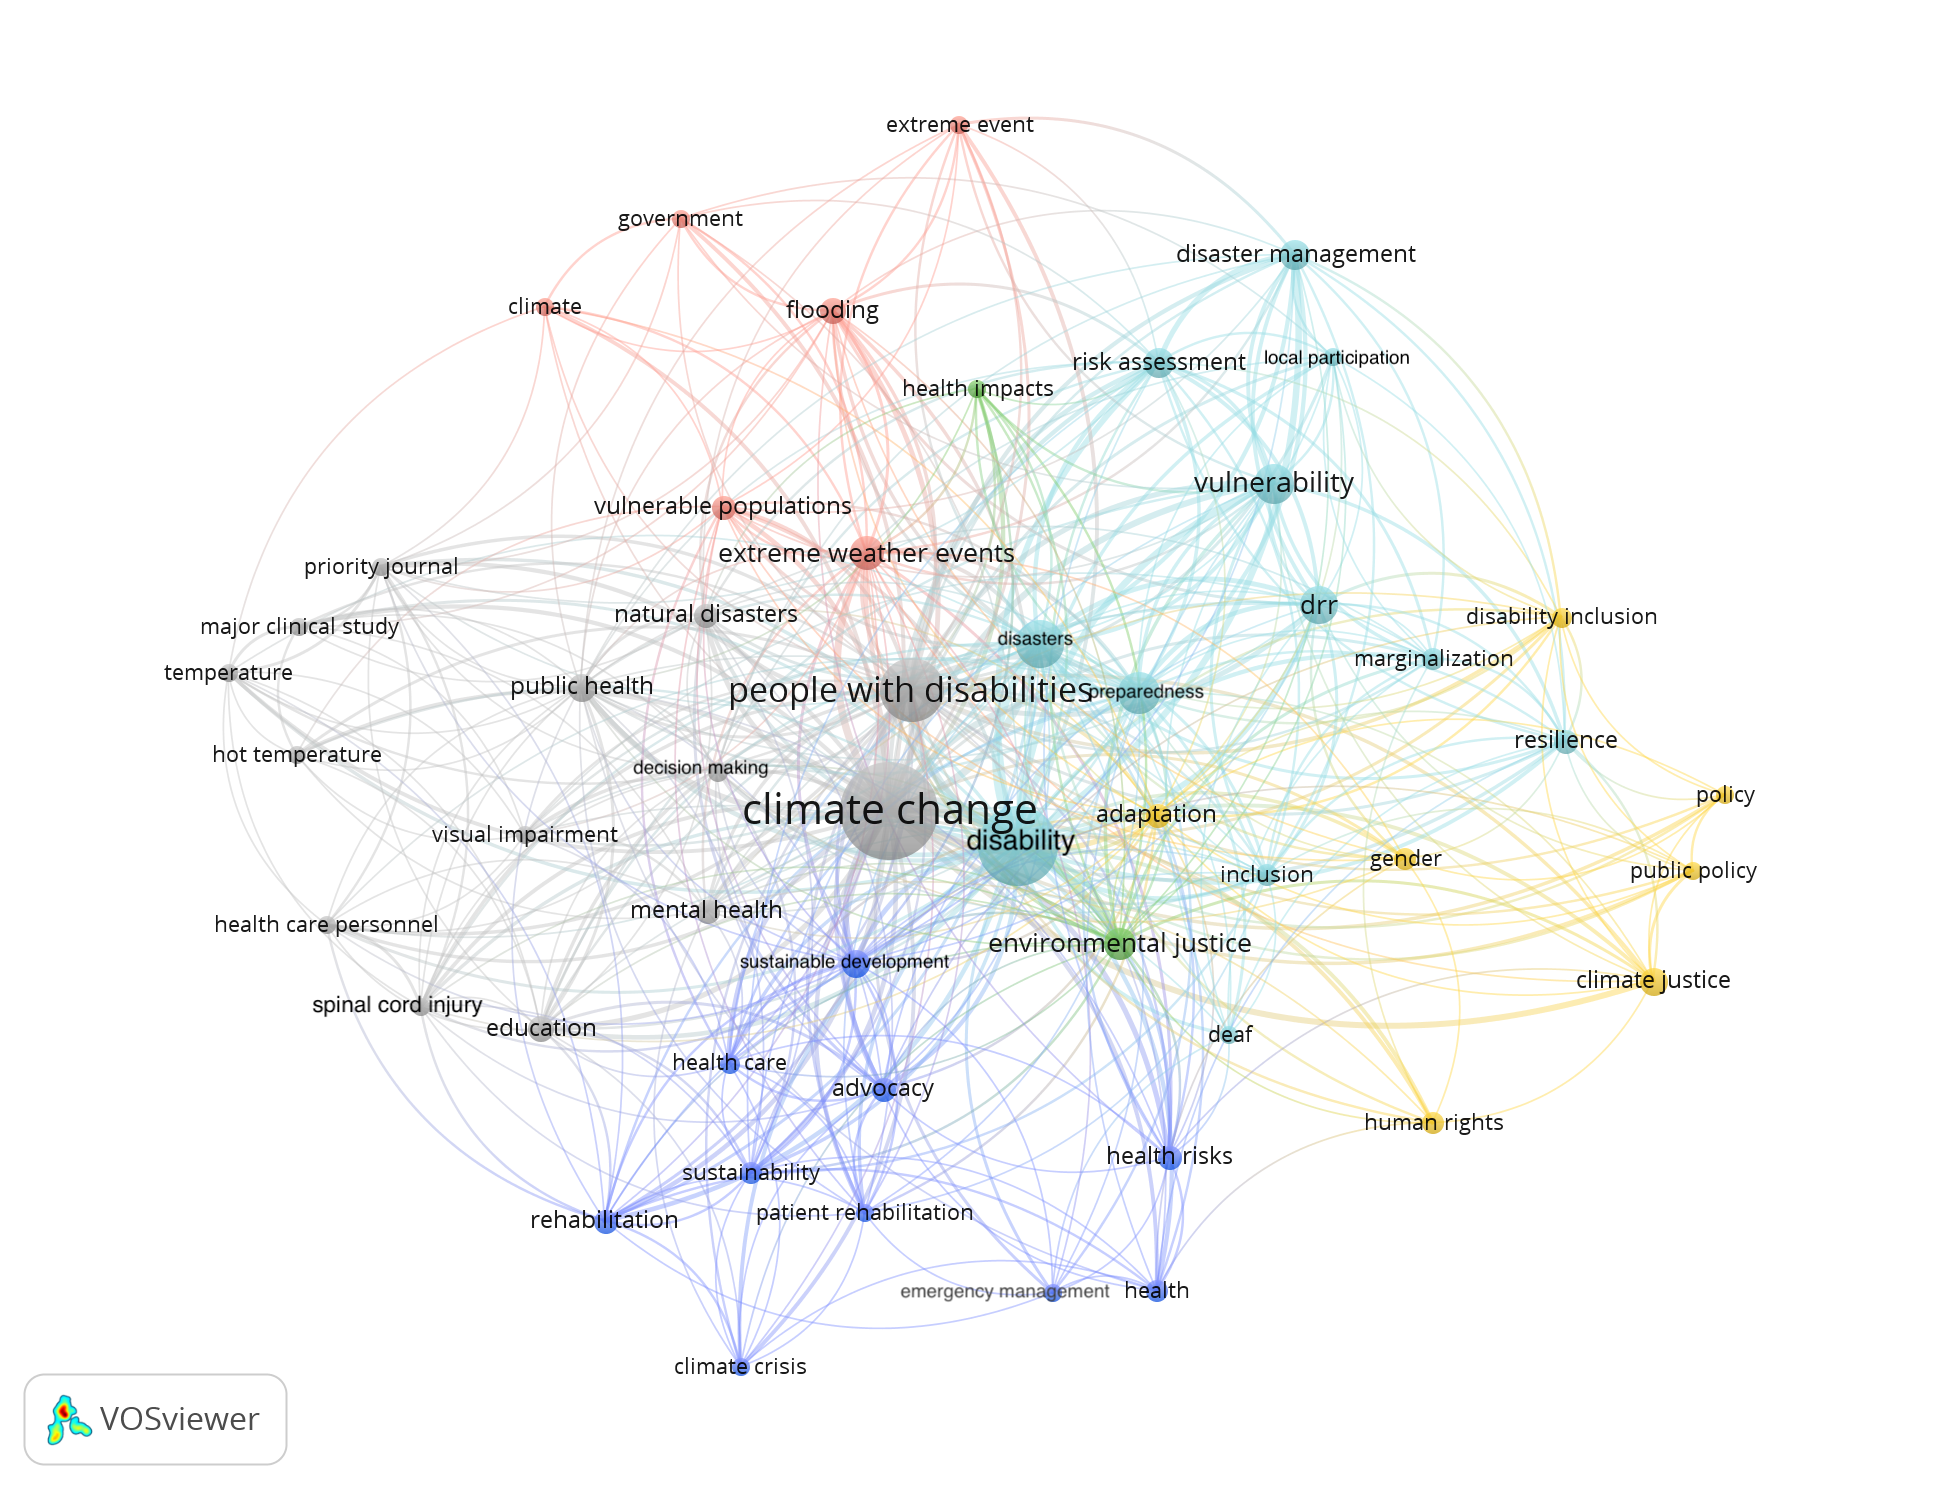
\includegraphics[width=1\textwidth]{network 0528.png}
    \caption{VOSviewer keyword co-occurrence network of the extended dataset.}
    \label{fig:enter-label}
\end{figure}

\subsection{Temporal evolution of research themes - VOSviewer}
Overlay visualisation positions keywords by co-occurrence and colours them by the average publication year of the documents in which they appear, allowing the analysis to identify themes associated with earlier or more recent stages of the field \cite{van_eck_waltman_2010_vosviewer,van_eck_waltman_2014_visualizing}. As shown in Figure 4.4, earlier themes cluster around vulnerability, risk assessment, disasters, public health and population categories (adults, women, children, older people), while more recent terms (climate justice with an average year of 2024.2, extreme weather, health risks, disaster prevention, adaptation, sustainable development) indicate a gradual shift from a narrower disaster-risk and vulnerability framing towards climate justice, adaptation and governance. Concepts directly related to policy evaluation, behavioural response and adaptive decision-making remain weak or absent as central themes. Although the literature is moving beyond vulnerability framing, it has not yet developed a strong focus on how PWDs make decisions, participate in policy processes or respond behaviourally to adaptation interventions.
\begin{figure}[H]
    \centering
    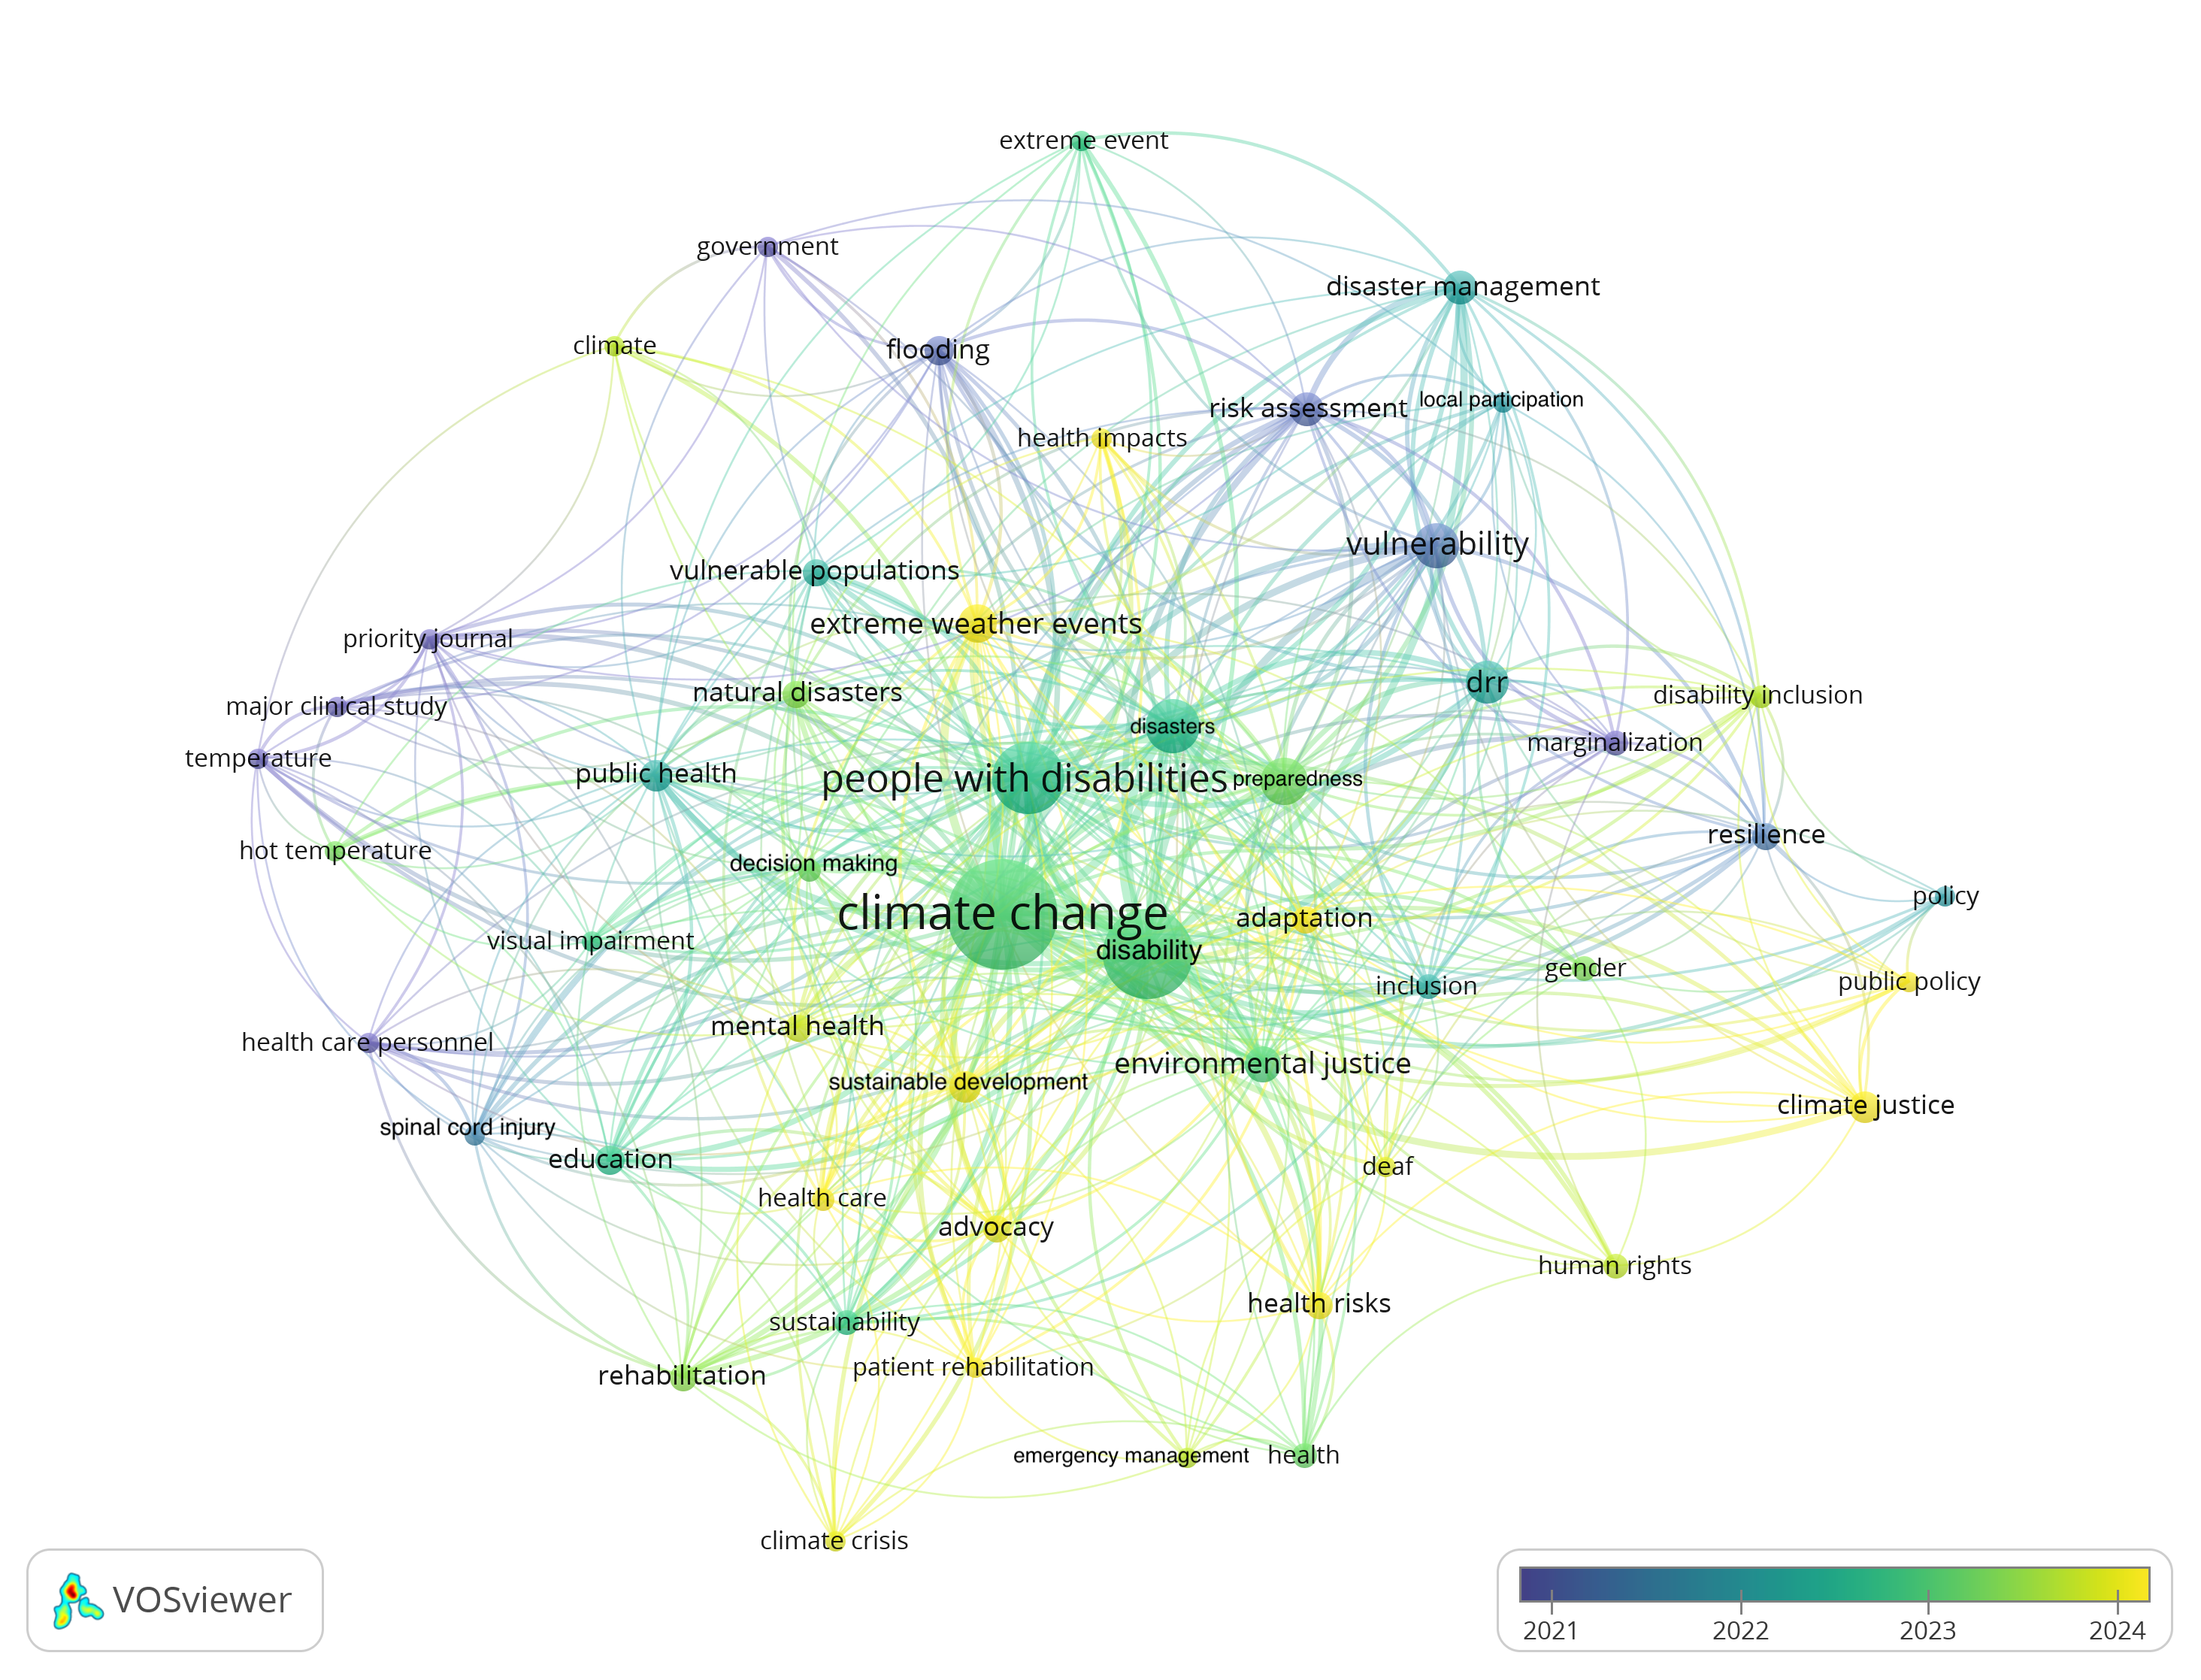
\includegraphics[width=0.7\textwidth]{Overlay 0528.png}
    \caption{Overlay Visualisation of Keyword Co-occurrence by Average Publication Year, 2006–2025}
    \label{fig:enter-label}
\end{figure}
\subsection{Network topology and community structure - Gephi}
The topological properties of the keyword network were calculated in Gephi. The network contains 60 nodes (keywords) and 615 edges (co-occurrence ties). Its graph density of 0.347 means that roughly a third of all possible keyword pairings actually co-occur, indicating that disability–climate research, while interdisciplinary, draws on a shared vocabulary rather than fragmenting into isolated terminologies. The average weighted degree of 51.8 reinforces this: dominant concepts such as disability, climate change and disasters are repeatedly anchored to a wide range of other terms (vulnerability, risk reduction, adaptation, environmental justice) rather than to a few specialised neighbours. The average clustering coefficient of 0.586, generating 2,421 triangles, denotes substantial local cohesion, the terms surrounding any one concept (around disaster risk reduction, for instance, preparedness, resilience, vulnerability and disaster management) themselves co-occur and form recognisable conceptual neighbourhoods. The network also forms a single connected component, so that even peripheral concepts such as deaf, spinal cord injury or local participation remain linked through intermediate terms to the dominant vocabulary, constituting an integrated knowledge structure rather than isolated subfields. Within this structure, disability, climate change and disasters serve as the conceptual anchors, with eigenvector centrality scores of 1.00, 0.98 and 0.89 respectively, terms that are not merely well connected but connected to other highly connected terms—so that almost every other concept gains its position by linking, directly or indirectly, to one of these three.

Modularity analysis examines the community structure of the keyword network, with higher scores indicating stronger separation between clusters \cite{newman_2006_modularity}.  The Gephi analysis identified two communities with a modularity score of 0.110. As shown in Figure 4.5, the first clusters around disasters, vulnerability, risk assessment, disaster management, preparedness, resilience and disaster risk reduction, reflecting a disability-disaster-risk framing. The second clusters around climate change, environmental justice, public health, sustainable development, adaptation, healthcare, mental health and human rights, reflecting a broader climate-health-governance framing. Climate change sits near the centre of the network and functions as a bridging concept, and the low modularity score shows that the two communities are interconnected rather than strongly separated. This partial separation between disability-focused disaster research and broader climate justice and adaptation governance research supports the need for a framework that more explicitly connects disability-specific behavioural evidence with climate adaptation policy evaluation.


\begin{figure}[H]
    \centering
    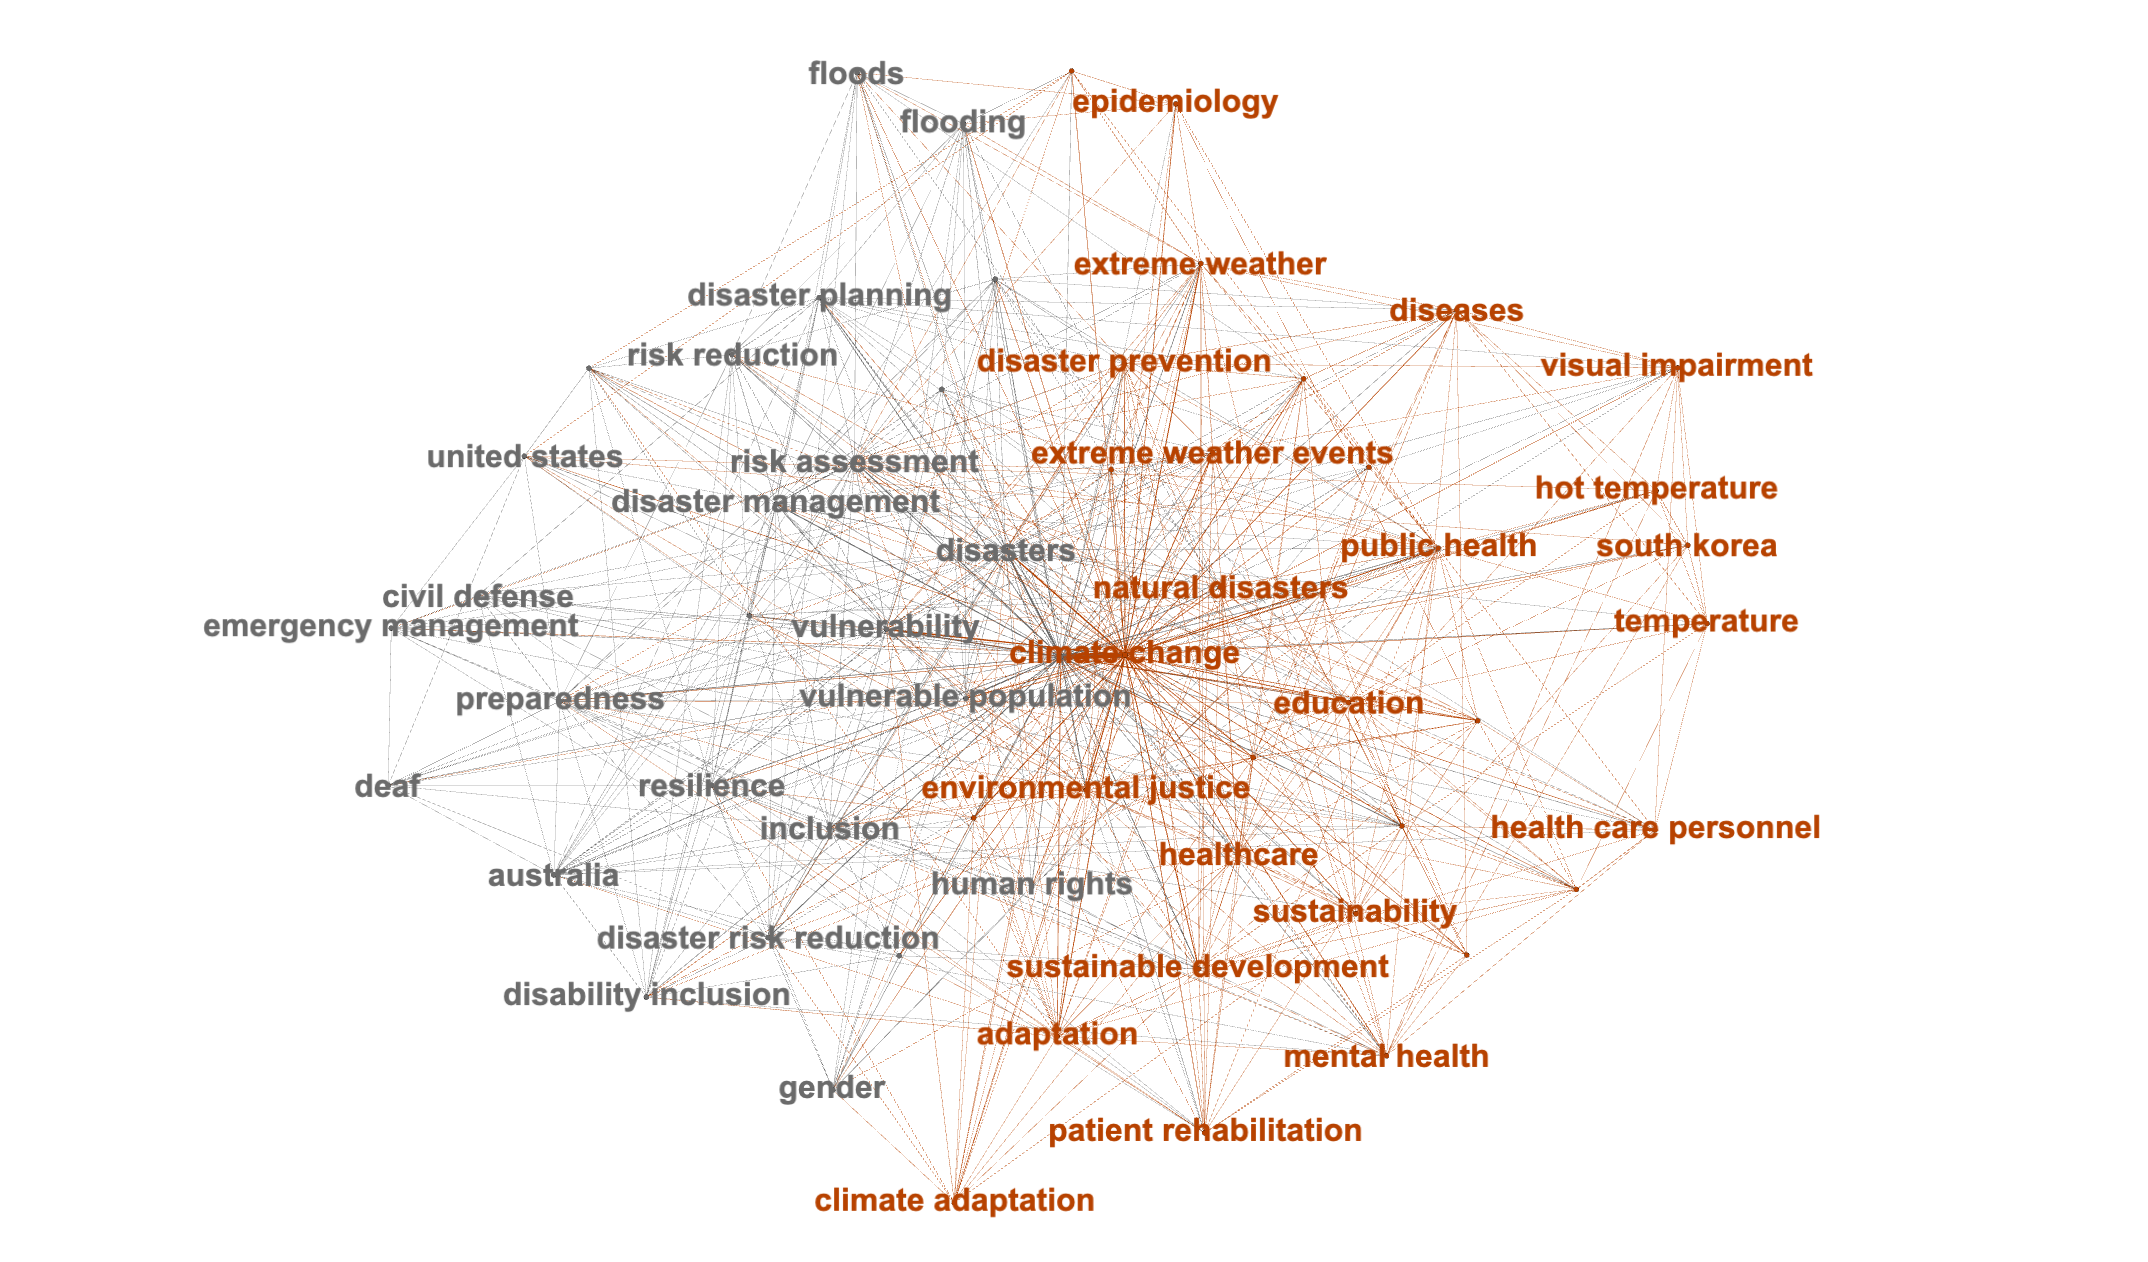
\includegraphics[width=1\textwidth]{Modularity.png}
    \caption{Gephi Modularity Visualisation of Keyword Co-occurrence Communities.}
    \label{fig:enter-label}
\end{figure}

\subsection{Summary of Bibliometric Findings}
Overall, the bibliometric analysis reveals a field centred on climate change, disability and persons with disabilities, with strong ties to disasters, vulnerability and risk reduction, but in which participation, decision-making, policy evaluation and disability inclusion remain noticeably more peripheral. The overlay analysis indicates a gradual shift towards climate justice, adaptation and governance, while the modularity analysis identifies two partially connected communities (disability-disaster-risk and climate-health-governance) bridged by climate change. Taken together, these results show that the field increasingly recognises disability within climate-related risks, yet has not connected disability-specific behavioural evidence to the evaluation of climate adaptation policy. This is precisely the gap the present study addresses.


\section{Topic Modelling}
Where the bibliometric analysis in Section~4.3 maps the macro-level structure and clustering of the literature, TM tests whether the documents themselves separate into substantively distinct thematic groups, using unsupervised learning over the combined titles, abstracts and author keywords of the 267-record extended dataset \cite{blei_2012_probabilistic,barde2017overview}. BERTopic was selected for the task because it combines transformer-based sentence embeddings with density-based clustering and a class-based TF-IDF scheme for keyword extraction, producing semantically coherent clusters even when documents use different terminology to describe related ideas \cite{grootendorst_2022_bertopic,reimers_2019_sentence}: well suited to a fragmented, interdisciplinary corpus where the same concern (for example, accessibility during disasters) surfaces under different vocabularies across rehabilitation medicine, environmental justice and DRR. The analysis below proceeds in four steps: how the topics were generated and labelled (Section~4.4.1), the relative importance of representative terms (Section~4.4.2), how topic prevalence has shifted over time (Section~4.4.3), and the annual publication trend of the modelled corpus (Section~4.4.4).
% \subsection{LDA Result}
% The LDA model was implemented in Python. After text pre-processing, different topic numbers were tested, and a six-topic solution was selected because it provided the clearest balance between interpretability and thematic distinction. Table 4.2 summarises the six topics, their representative keywords, interpreted labels and relevance to the PhD research gap. The topics cover disability-inclusive disaster risk reduction and rights (Topic 1), rights and disability-specific communication (Topic 2), heat and environmental health impacts (Topic 3), disaster preparedness and emergency planning (Topic 4), adaptation, social vulnerability and environmental justice (Topic 5), and environmental health and psychosocial impacts (Topic 6). Overall, the literature appears to be organised around disaster risk, health impacts, environmental exposure, adaptation and justice — distributed across several partially overlapping research framings rather than dominated by a single thematic concern.

% \begin{table}[htbp]
% \centering
% \footnotesize
% \renewcommand{\arraystretch}{1.35}
% \caption{Preliminary LDA topic modelling results and interpreted topic labels}
% \label{tab:lda-topic-modelling-results}

% \begin{tabularx}{\textwidth}{
% >{\raggedright\arraybackslash}p{1.8cm}
% >{\raggedright\arraybackslash}p{3.2cm}
% >{\raggedright\arraybackslash}X
% >{\raggedright\arraybackslash}X
% }
% \toprule
% \textbf{Topic} & \textbf{Representative keywords} & \textbf{Interpreted topic label} & \textbf{Relevance to the PhD gap} \\
% \midrule

% Topic 1
% & disaster, risk, inclusive, reduction, rights
% & Disability-inclusive disaster risk reduction and rights
% & Shows the importance of disaster risk reduction frameworks, but the focus remains more on risk and inclusion than on behavioural policy response \\

% Topic 2
% & rights, deaf, human, disaster, access
% & Rights, access and disability-specific communication
% & Highlights rights, access and communication barriers, especially for specific disability groups \\

% Topic 3
% & health, temperature, care, extreme, heat
% & Heat, care and environmental health impacts
% & Shows concern with heat exposure, care needs and health impacts of climate-related hazards \\

% Topic 4
% & disaster, preparedness, risk, planning, management
% & Disaster preparedness and emergency planning
% & Indicates a strong focus on preparedness, emergency planning and disaster management \\

% Topic 5
% & health, adaptation, social, environmental, justice
% & Adaptation, social vulnerability and environmental justice
% & Represents the topic most closely aligned with climate justice and adaptation governance \\

% Topic 6
% & environmental, health, events, mental, extreme
% & Environmental health and psychosocial impacts
% & Indicates attention to environmental events, mental health and broader health impacts \\

% \bottomrule
% \end{tabularx}
% \end{table}

% The keyword distribution across the six LDA topics is shown in Figure 4.6. Topics 1 and 4 are both disaster-related but capture distinct emphases: Topic 1 is more closely associated with inclusive disaster risk reduction, rights and DRR frameworks, whereas Topic 4 focuses on preparedness, emergency planning and disaster management. Topic 3 is centred on heat, temperature and care, while Topic 5 links adaptation, social vulnerability and environmental justice most directly to the governance concerns of this PhD.

% \begin{figure}[H]
%   \centering
%   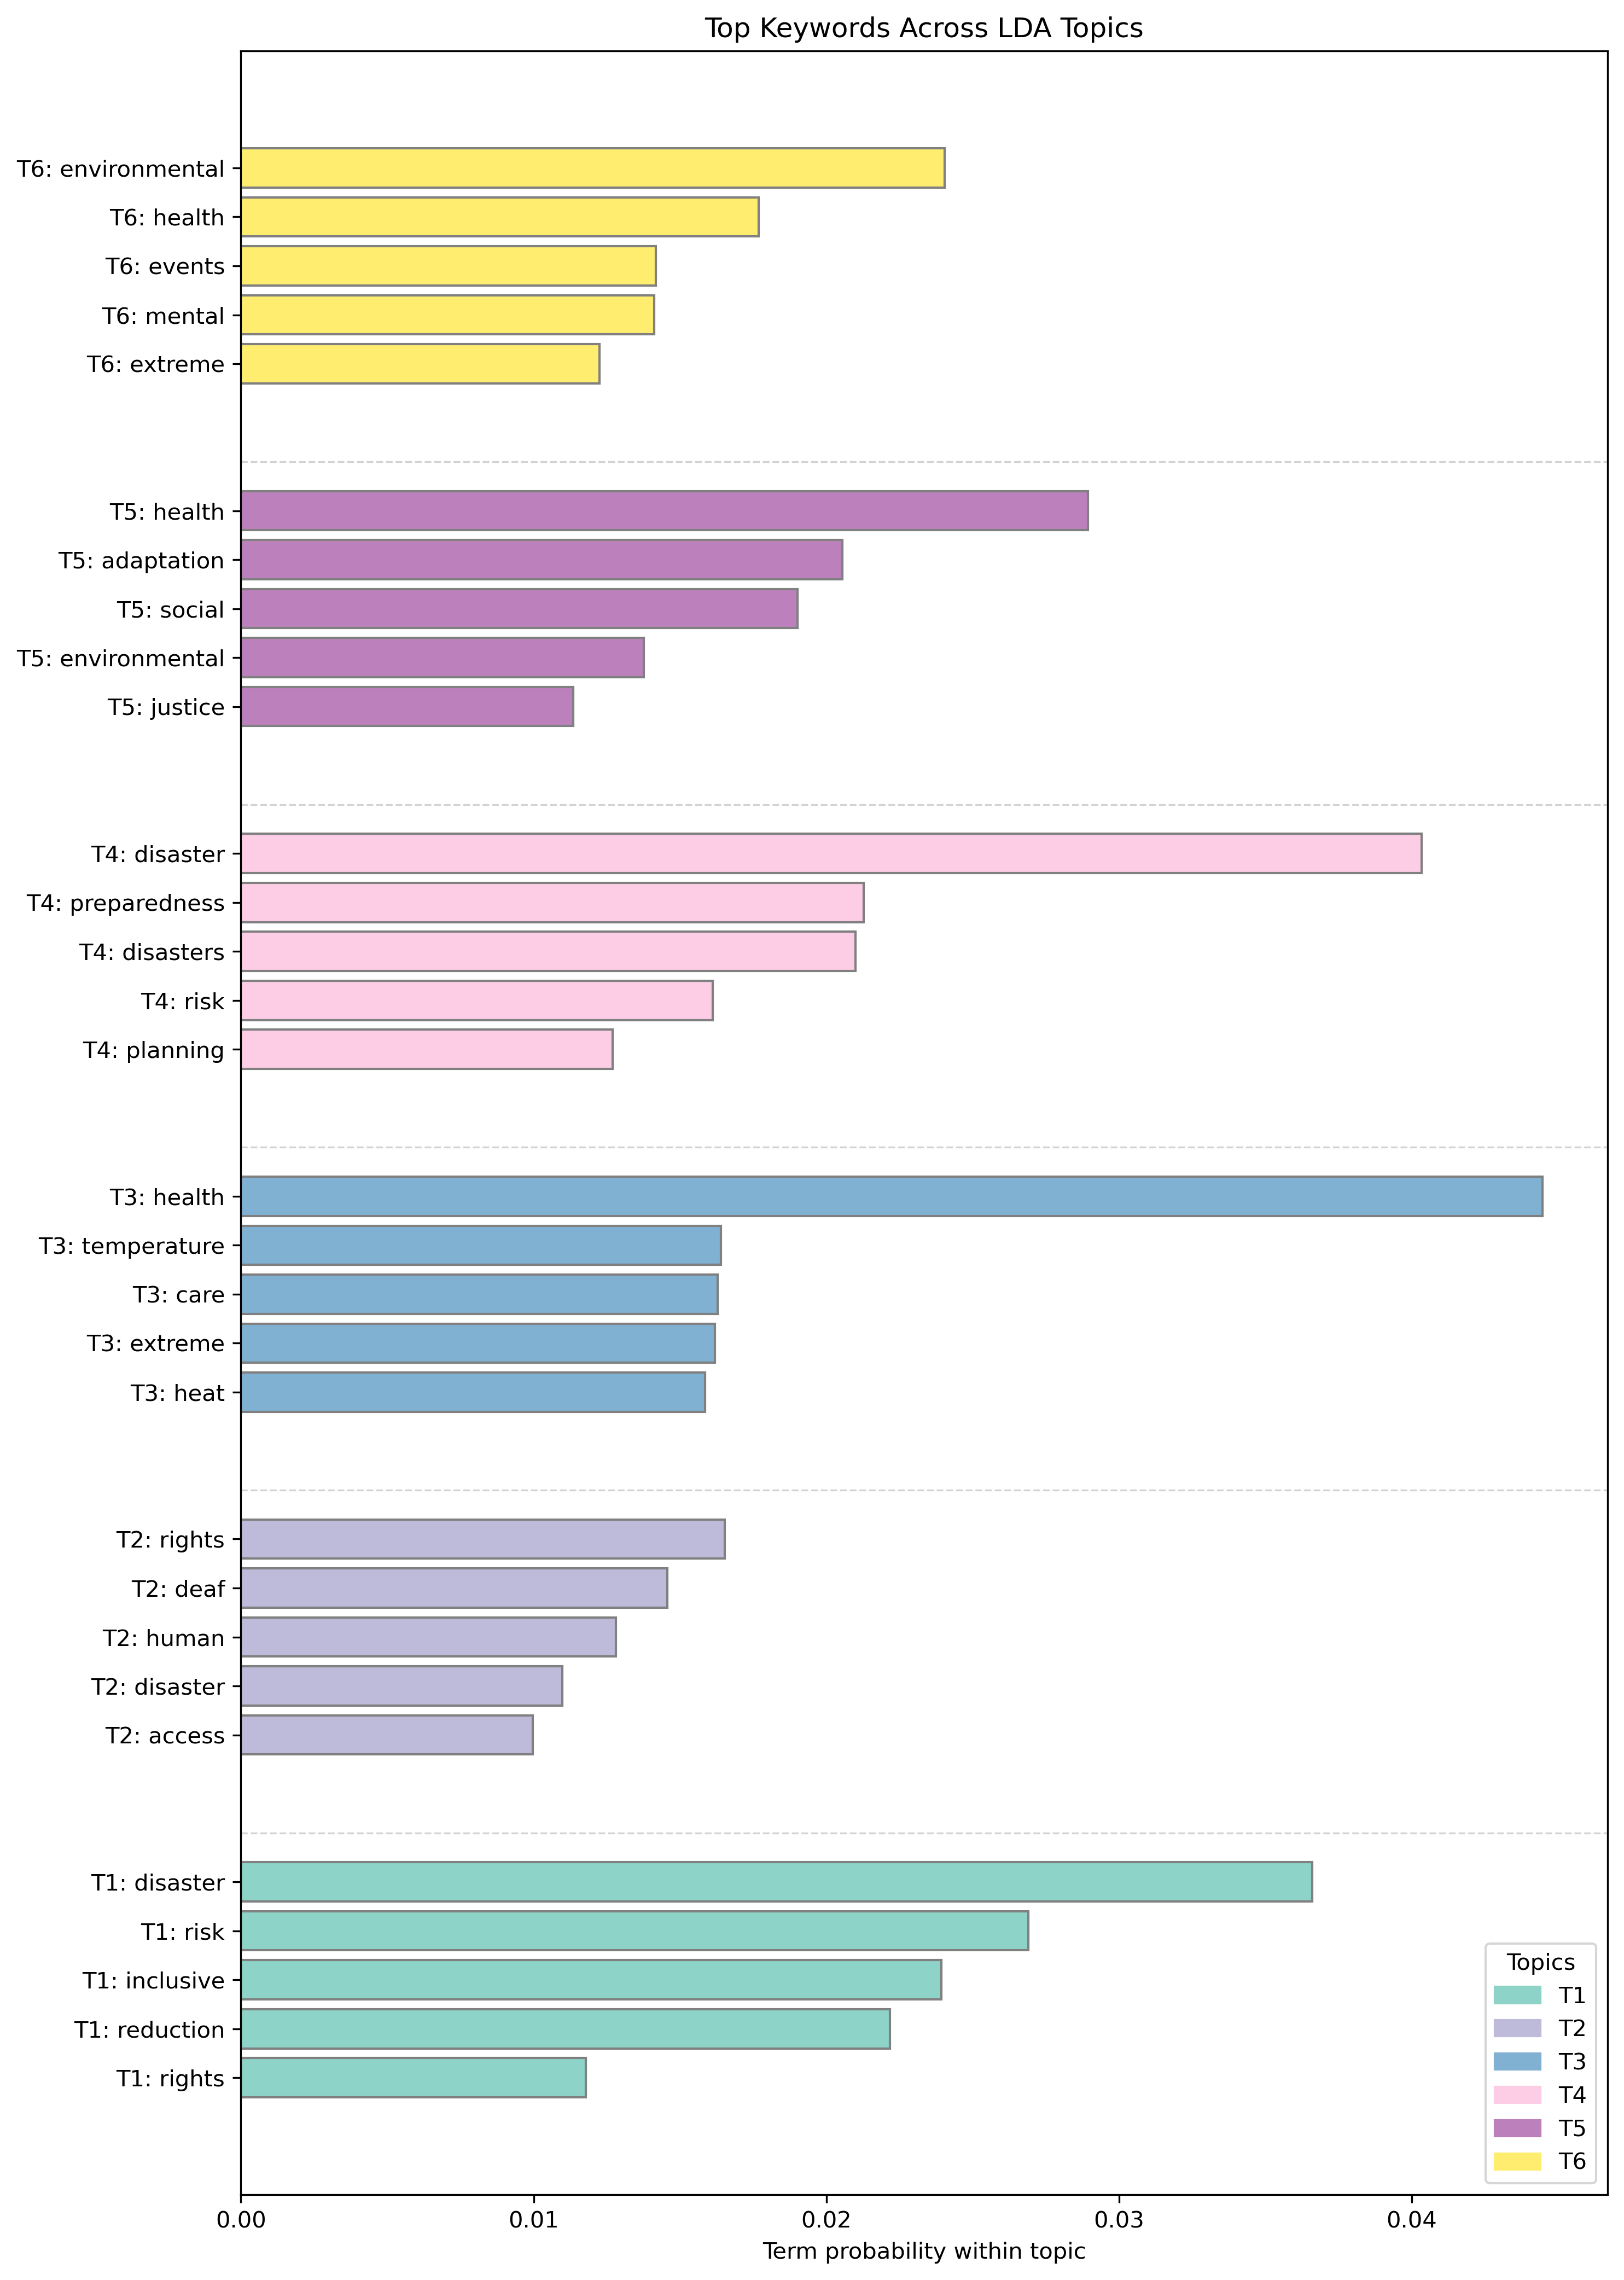
\includegraphics[width=0.7\textwidth]{lda_all_topics_keywords.png}
%   \caption{Top keywords across the six LDA topics by term probability}
%   \label{fig:lda_keywords}
% \end{figure}

% The distribution of articles across the six topics is shown in Figure 4.5. Topic 1, disability-inclusive disaster risk reduction and rights, is the largest topic (n=65), followed by Topic 5, adaptation, social vulnerability and environmental justice (n=59). Topic 6, environmental health and psychosocial impacts, is the smallest (n=23) but remains thematically distinct. This distribution suggests that disaster risk reduction and adaptation/environmental justice form the two most visible thematic strands in the dataset, while the presence of multiple medium-sized topics confirms that the field is structured around several analytically distinct but interconnected framings.

% \begin{figure}[H]
%   \centering
%   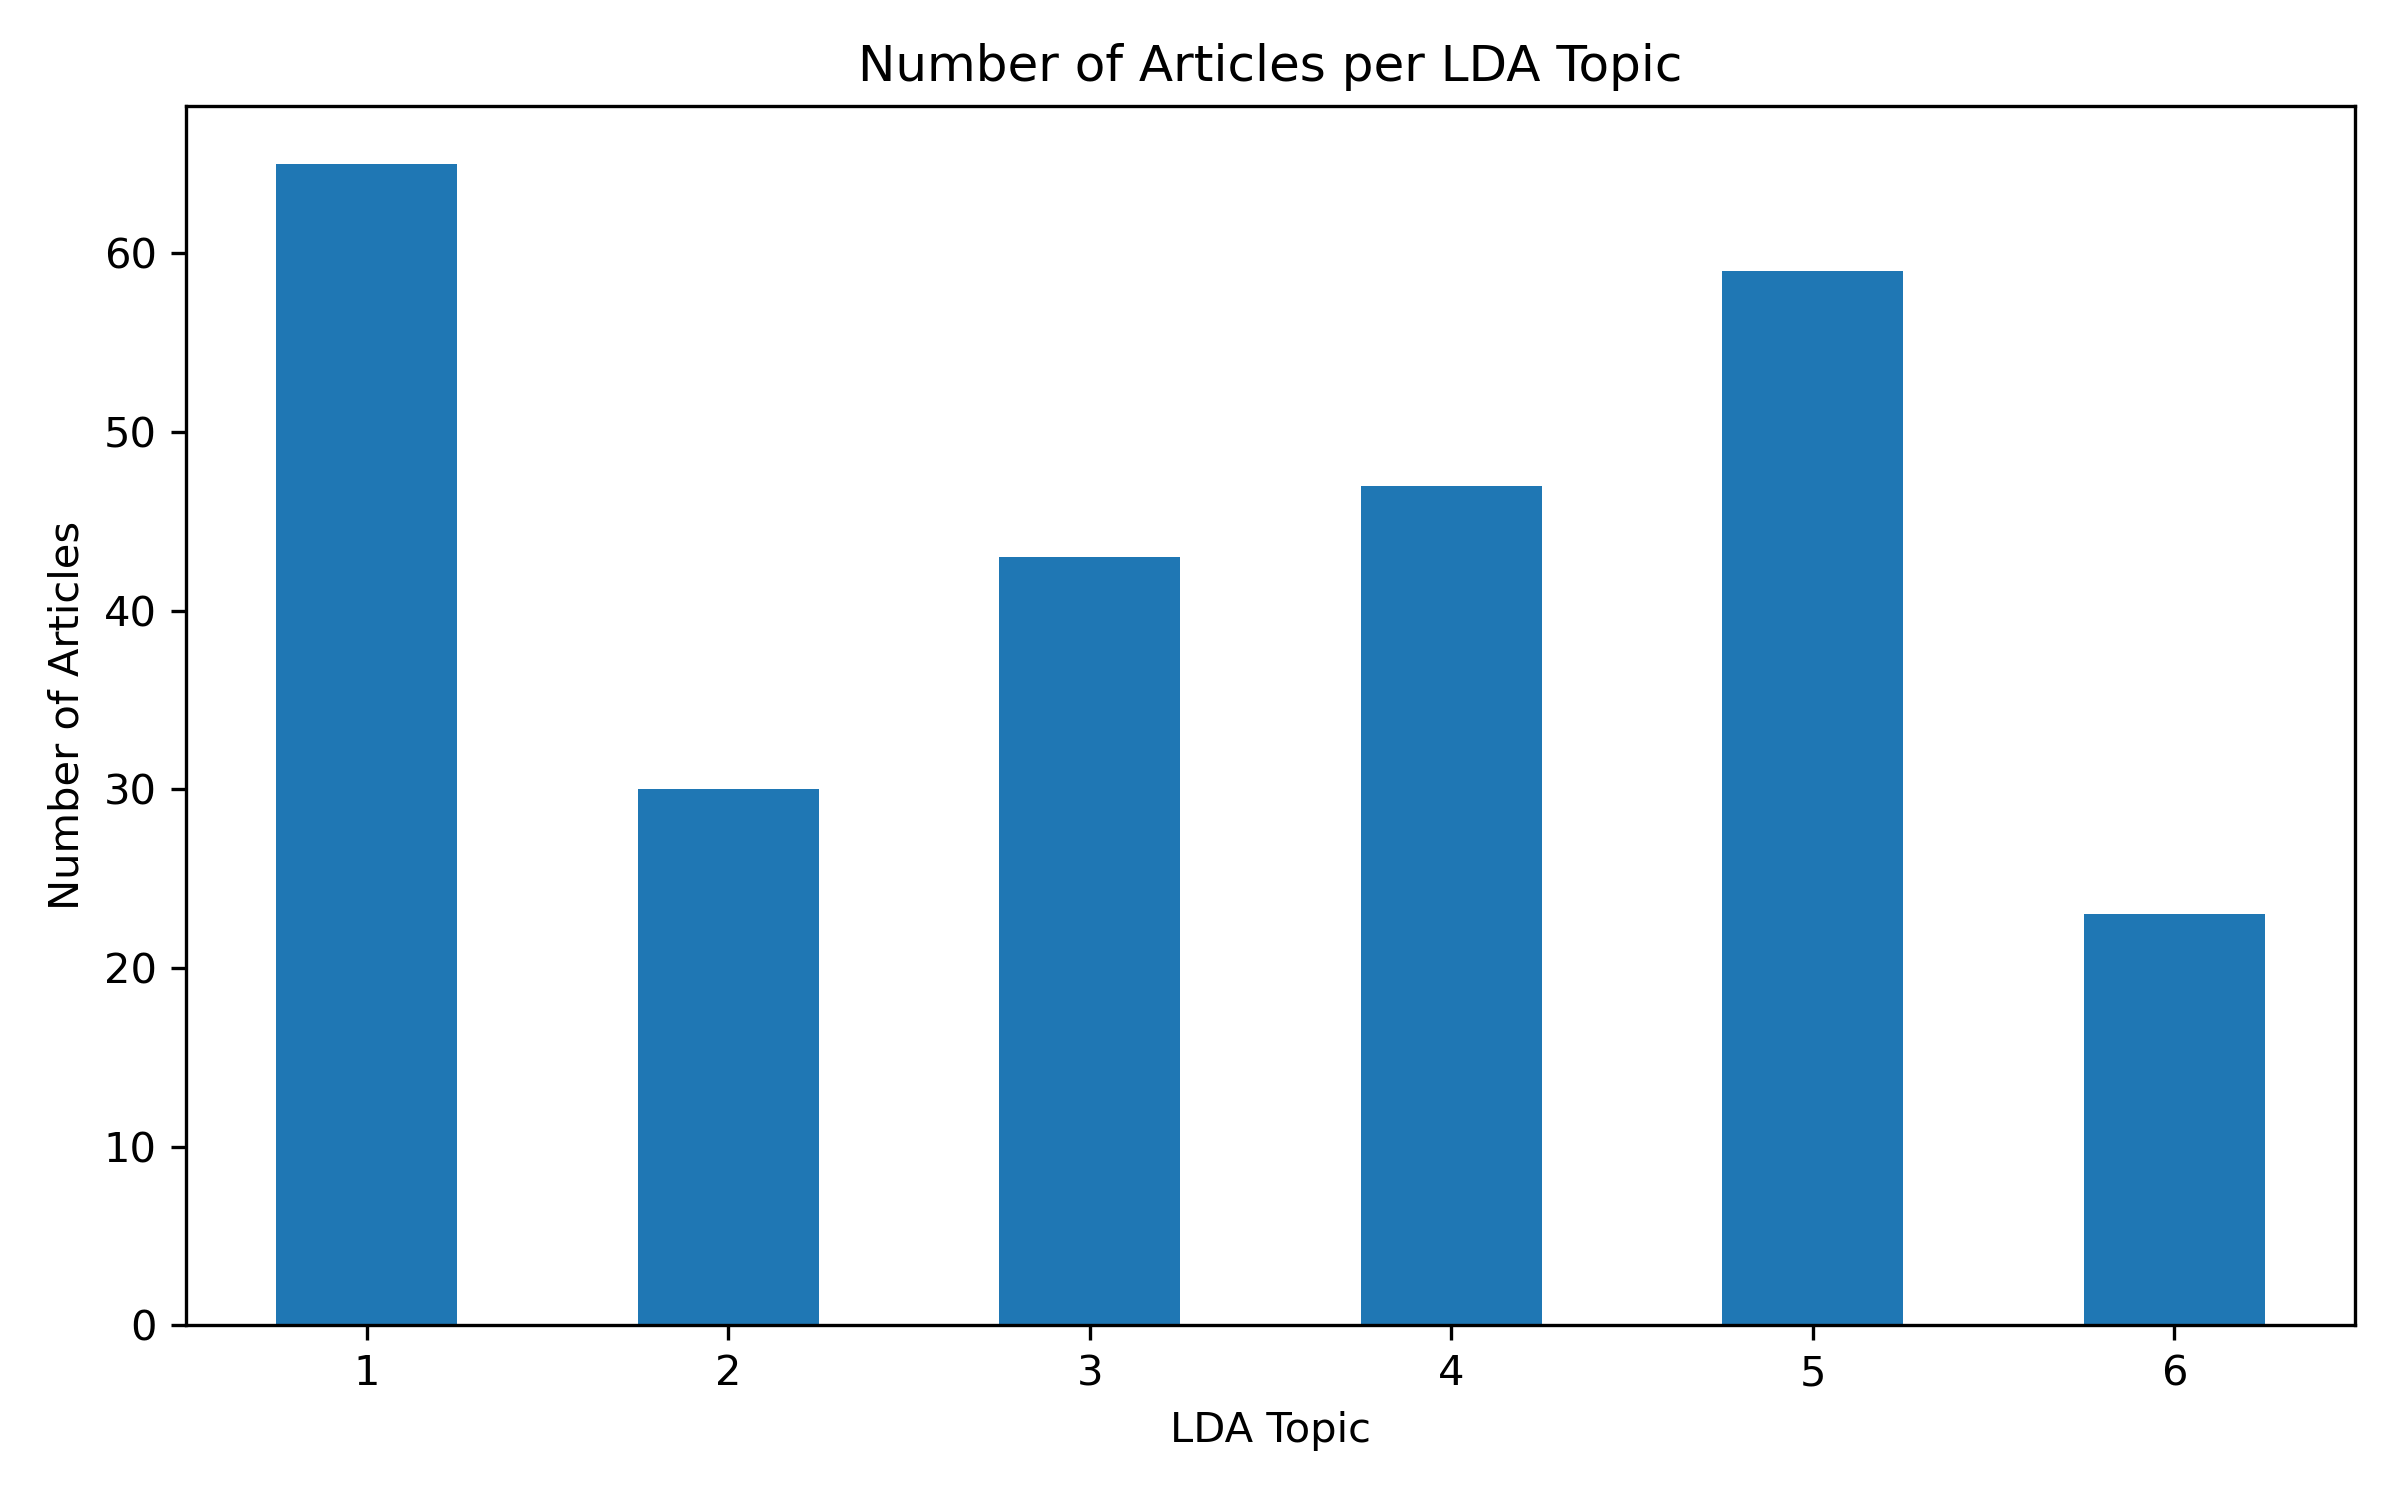
\includegraphics[width=\textwidth]{lda_topic_size.png}
%   \caption{Number of articles per LDA topic}
%   \label{fig:lda_size}
% \end{figure}

% The temporal distribution of topics is shown in Figure 4.6. Publication activity across all six topics remains low before 2019, with a marked increase after 2020 and a particularly sharp rise in 2024--2025. The strongest recent growth appears in topics related to disaster risk reduction, environmental health impacts and adaptation/environmental justice. This temporal pattern should be interpreted cautiously, as recent years may be affected by database coverage and publication timing. Nevertheless, the post-2020 increase suggests that disability is receiving substantially greater attention within climate-related research in recent years.
% \begin{figure}[H]
% \centering
% 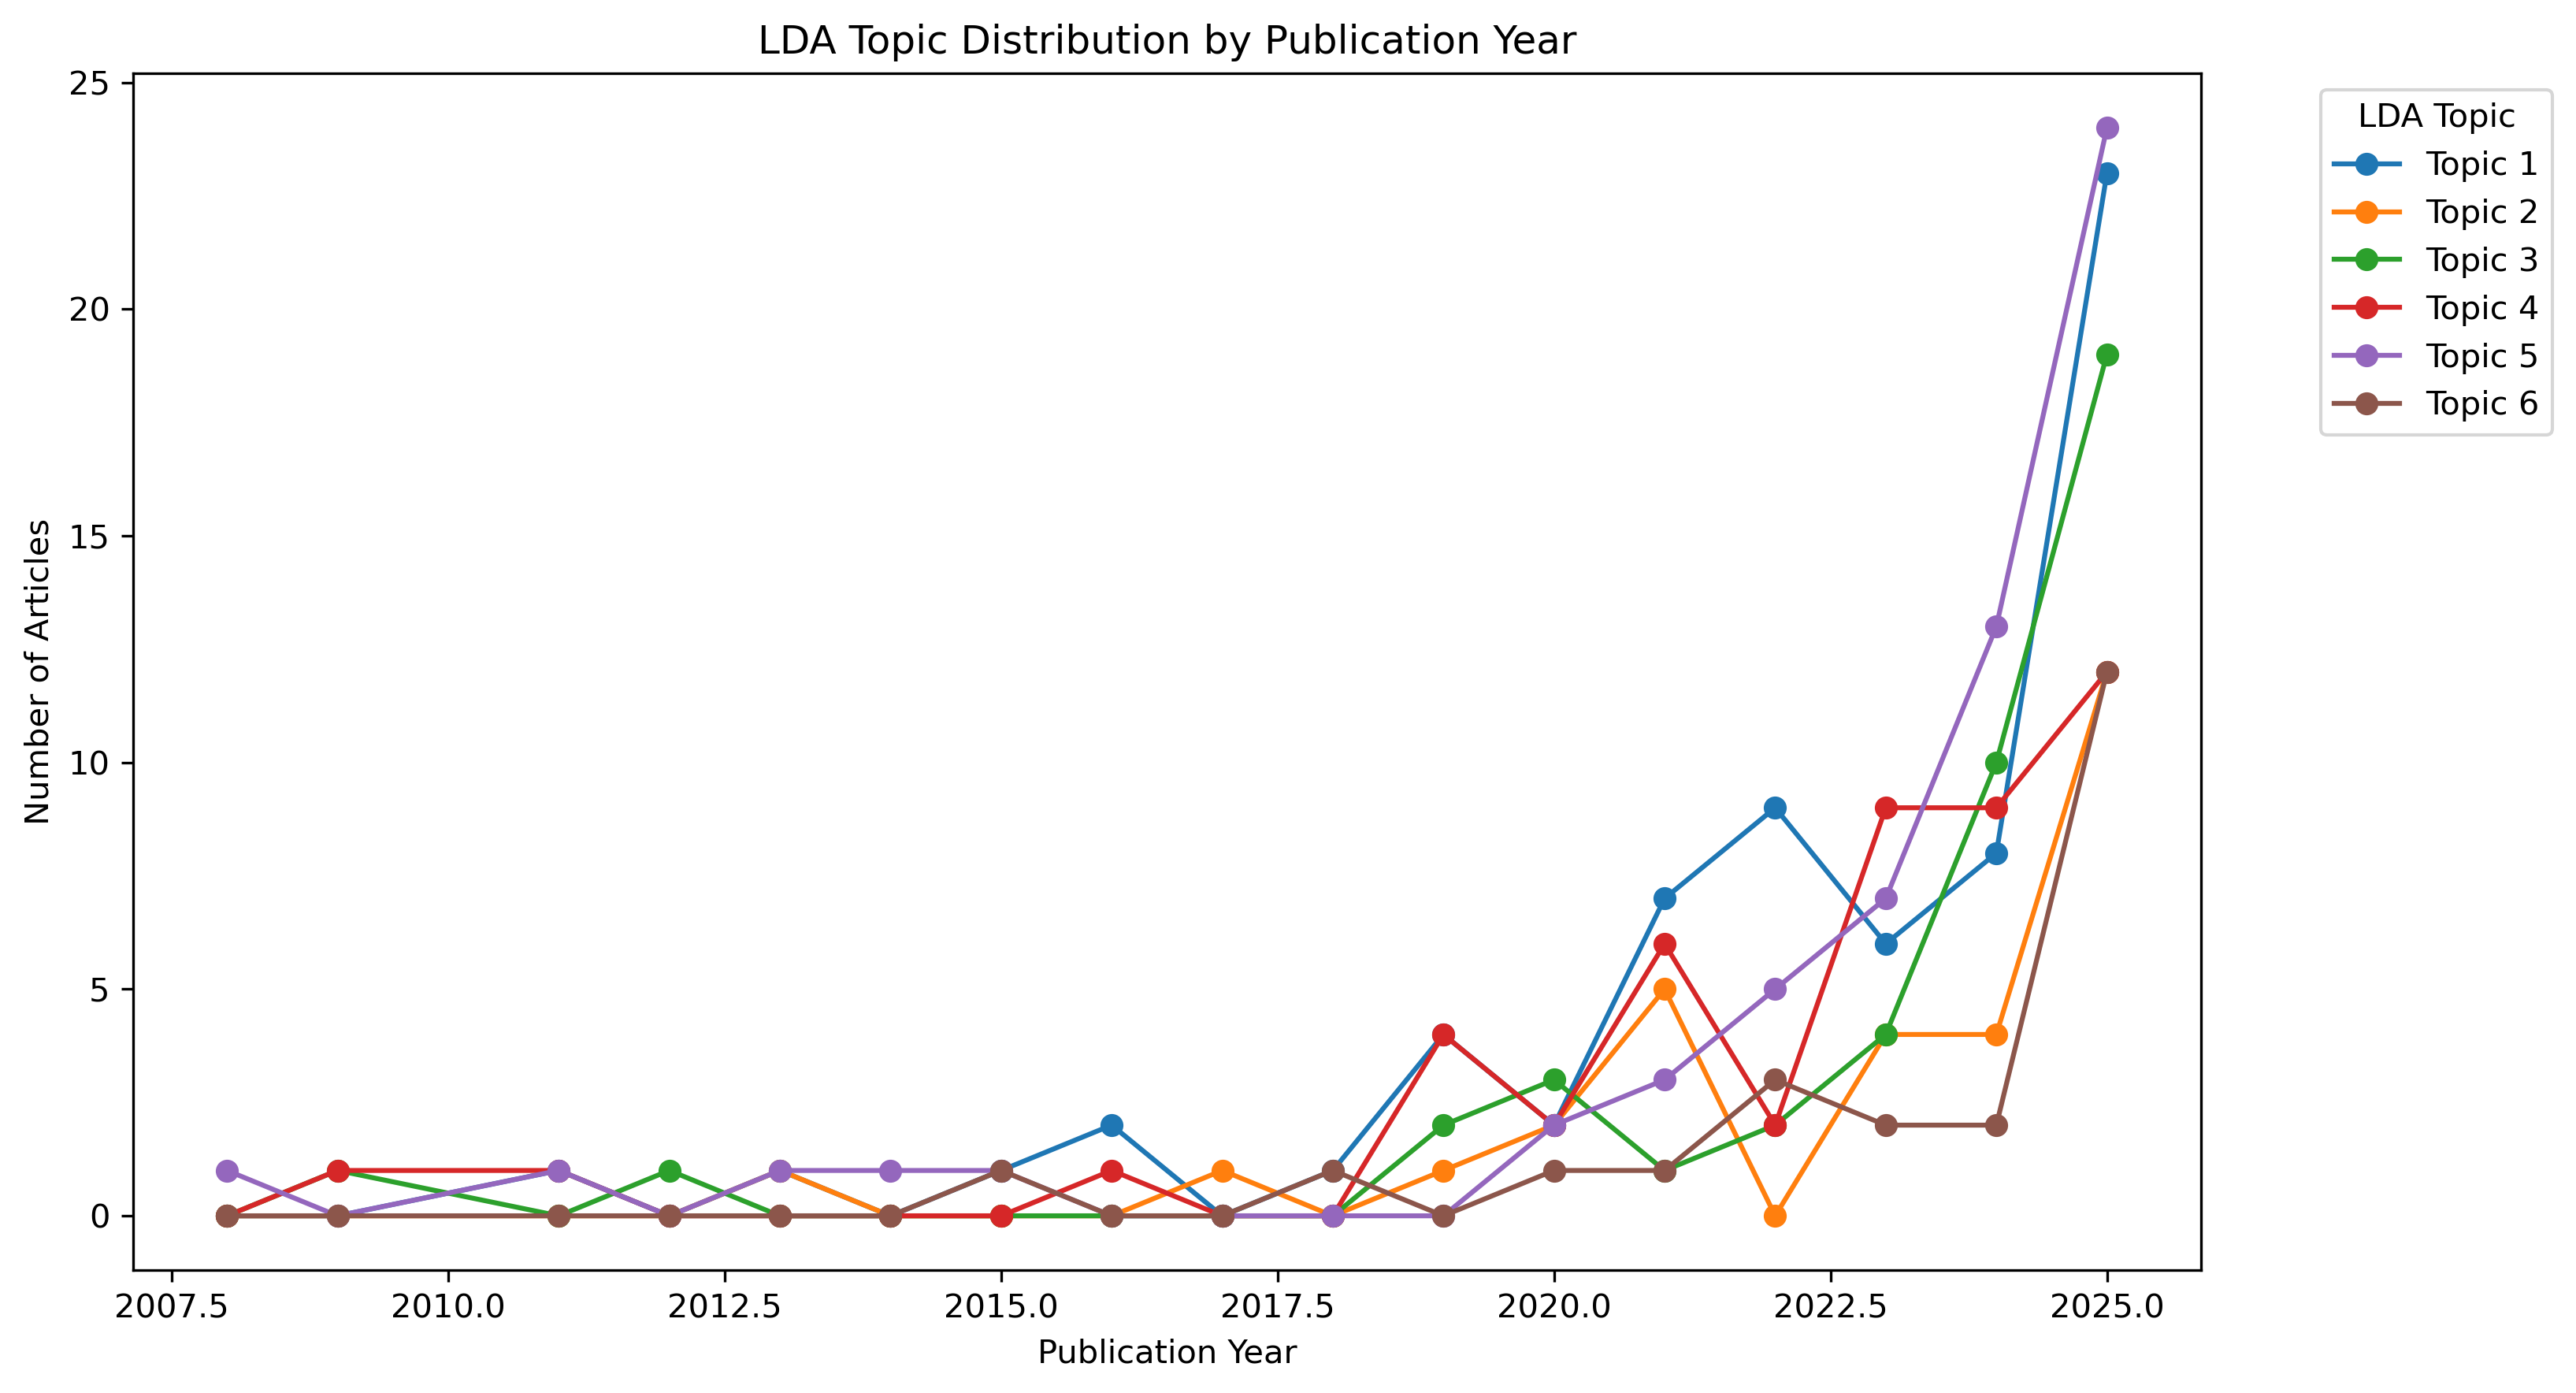
\includegraphics[width=\textwidth]{lda_topic_by_year.png}
% \caption{LDA topic distribution by publication year}
% \label{fig:lda_temporal}
% \end{figure}
% The conceptual relationships between the six topics are shown in the intertopic distance map in Figure 4.7. Topics 5 and 6 are positioned close to each other, indicating thematic overlap around environmental health, vulnerability and adaptation. Topic 3 appears relatively isolated, suggesting a more distinct focus on heat and health-related exposure. Topics 1 and 4 are both related to disaster risk, but their spatial separation reflects a distinction between rights-oriented DRR and more operational preparedness and planning concerns.
% \begin{figure}[H]
% \centering
% 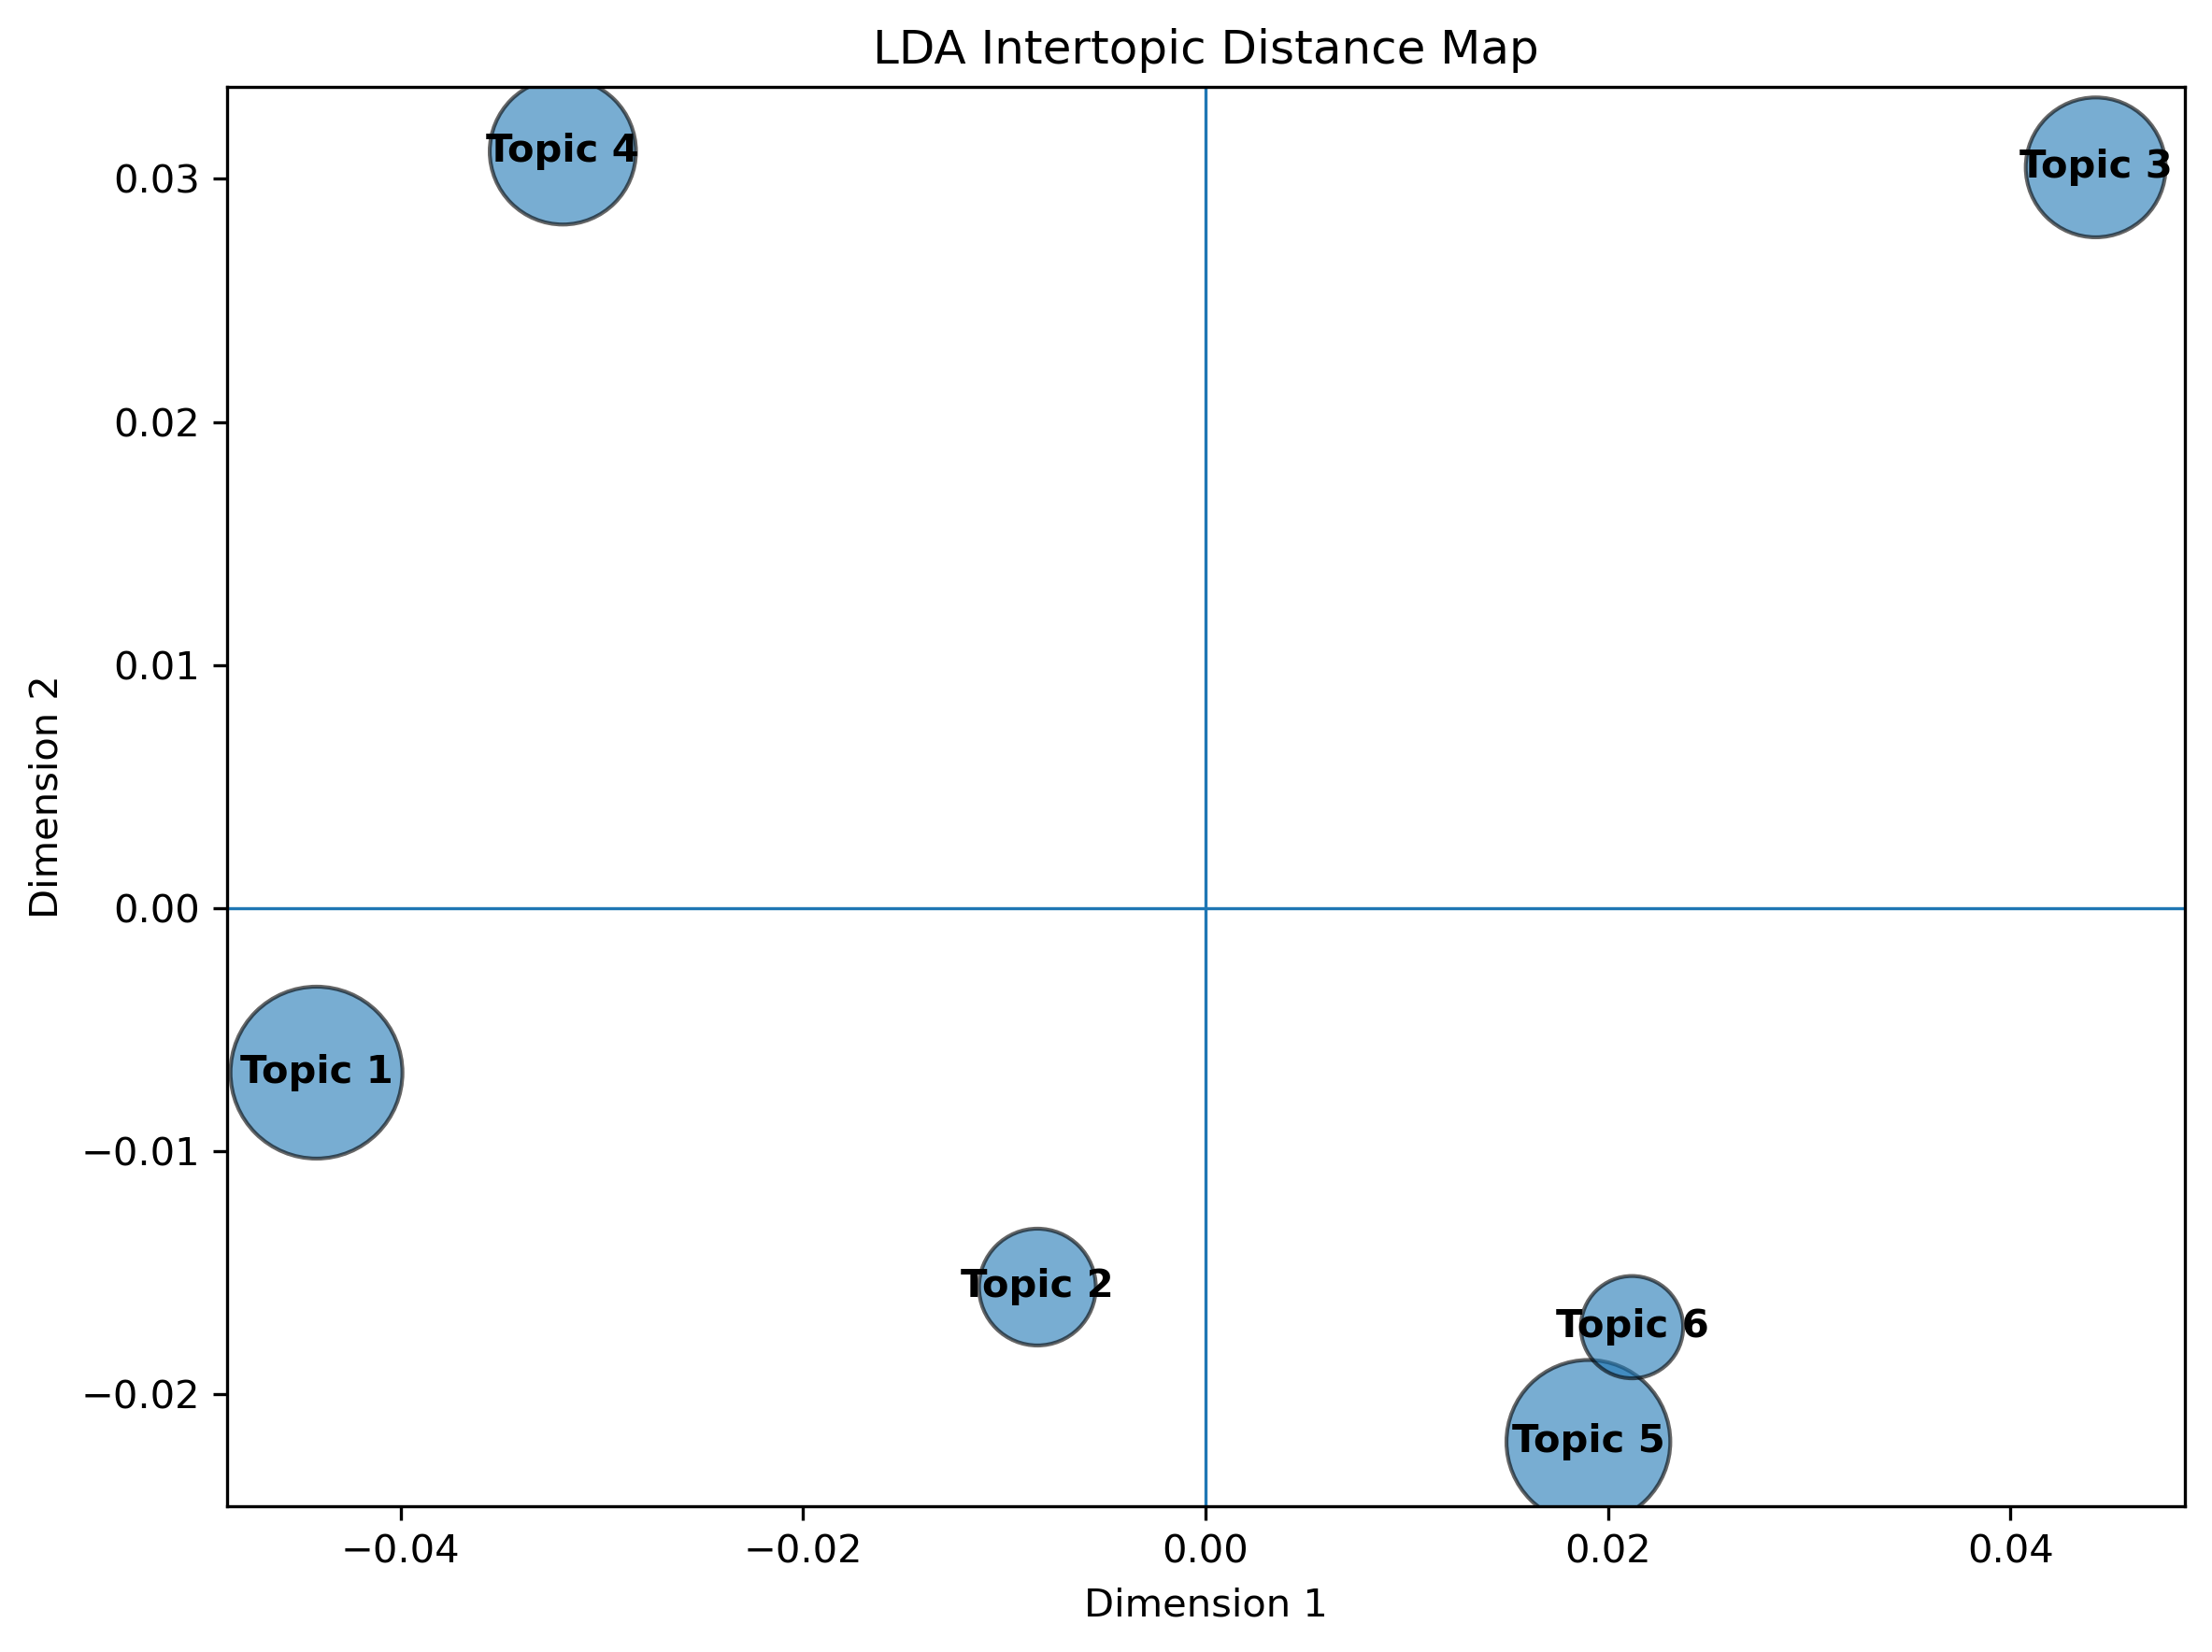
\includegraphics[width=\textwidth]{lda_intertopic_map.png}
% \caption{LDA intertopic distance map of the six-topic solution}
% \label{fig:lda_intertopic}
% \end{figure}
\subsection{Topic generation and labelling process}
Since the labelling of each topic rests on its representative keywords, it is useful to clarify how those keywords were selected. Once documents had been clustered, BERTopic produced a ranked list of terms for each cluster using class-based TF-IDF \cite{grootendorst_2022_bertopic}, an extension of standard term-frequency and inverse-document-frequency weighting \cite{sparck_jones_1972_tfidf,salton_buckley_1988_termweighting} in which each topic is treated as a single class so that terms distinctive to a cluster rank above those merely common in the dataset. Top-ranked terms were then inspected for residual noise: where a generic or methodological term recurred across multiple topics and obscured their substantive content, it was added to the stop-word list and the model re-fitted. This was repeated until the keyword profile of each cluster was distinctive enough to support a meaningful manual label; the lists reported in Table~\ref{tab:bertopic_topics} therefore reflect the iterated output rather than the raw first-pass model.

The model was implemented in Python and, after pre-processing, generated nine interpretable topics from the 267-record extended dataset. Topics were reviewed through a combined interpretation of representative keywords, topic-word scores, topic size and document content, and labelled manually according to their substantive meaning within the disability and climate change literature. Table~\ref{tab:bertopic_topics} provides an initial thematic overview before the following figures examine term importance, topic distribution and topic prevalence over time.

\begin{table}[H]
\centering
\small
\renewcommand{\arraystretch}{1.3}
\caption{BERTopic-generated topics and representative keywords}
\label{tab:bertopic_topics}

\begin{tabularx}{\textwidth}{
>{\raggedright\arraybackslash}p{0.13\textwidth}
>{\raggedright\arraybackslash}X
>{\raggedright\arraybackslash}X
}
\toprule
\textbf{Topic} & \textbf{Interpreted label} & \textbf{Representative keywords} \\
\midrule

Topic 1
& disaster risk and risk reduction
& disaster; risk; reduction; disability; inclusive; preparedness; drr \\

Topic 2
& rights, environmental justice and adaptation
& rights; disability; environmental; adaptation; justice; inclusive; policy; social; vulnerability; policies \\

Topic 3
& heat and environmental health impacts
& temperature; heat; health; air; multiple sclerosis; pollution; air pollution \\

Topic 4
& health, design and disability-related impacts
& health; design; disability; impact; persons w/ disabilities; sustainable; environmental; systems; interventions; inclusive \\

Topic 5
& justice, equity and legal adaptation
& justice; adaptation; indigenous; equity; legal; marginalized; litigation; vulnerable; policy; law \\

Topic 6
& rehabilitation, medicine and care
& rehabilitation; health; medicine; care; physical medicine; physical; medicine rehabilitation; patients; professionals \\

Topic 7
& disease, health costs and government response
& disease; health; rare; government health; cost; health care; letter; tract; pandemics; humans \\

Topic 8
& hurricanes, storms and living conditions
& hurricane; stroke; storm; living; cyclones; preparedness; injury; traumatic \\

Topic 9
& insurance, floods and extreme weather risk
& insurance; flood; risk; extreme weather; disability; environmental; weather; vulnerability; individuals \\

\bottomrule
\end{tabularx}
\end{table}
The topic labels were not produced automatically by the model, but were assigned through manual interpretation of the representative terms and document clusters. This step was necessary because BERTopic identifies statistically and semantically coherent clusters, while the substantive meaning of each topic still requires interpretation in relation to the research context. The table therefore provides the basis for the following analysis of word importance within each topic, topic prevalence over time, and the annual publication trend of the modelled corpus.

\subsection{Term importance within each topic}
Figure~\ref{fig:bertopic_barchart} reports the term-importance bar chart produced by BERTopic for each of the nine substantive clusters. Terms are ranked by their class-based TF-IDF score \cite{grootendorst_2022_bertopic}, a relative weight that combines how often a term appears within a topic with how rare it is across the rest of the corpus. Higher bars therefore identify terms that are both representative of a topic and distinctive to it, but absolute scores are not directly comparable across topics, since each topic is scored against its own frequency distribution.

Read alongside Table~\ref{tab:bertopic_topics}, the chart distinguishes two kinds of topic. Disaster, hazard and health specific clusters (Topics 1, 3, 6, 8 and 9) are anchored by a small set of technical terms that strongly differentiate them from the rest of the corpus, while cross cutting clusters (Topics 2 and 5) draw on a broader rights and governance vocabulary, reflected in their longer lists of representative terms.

\begin{figure}[H]
  \centering
  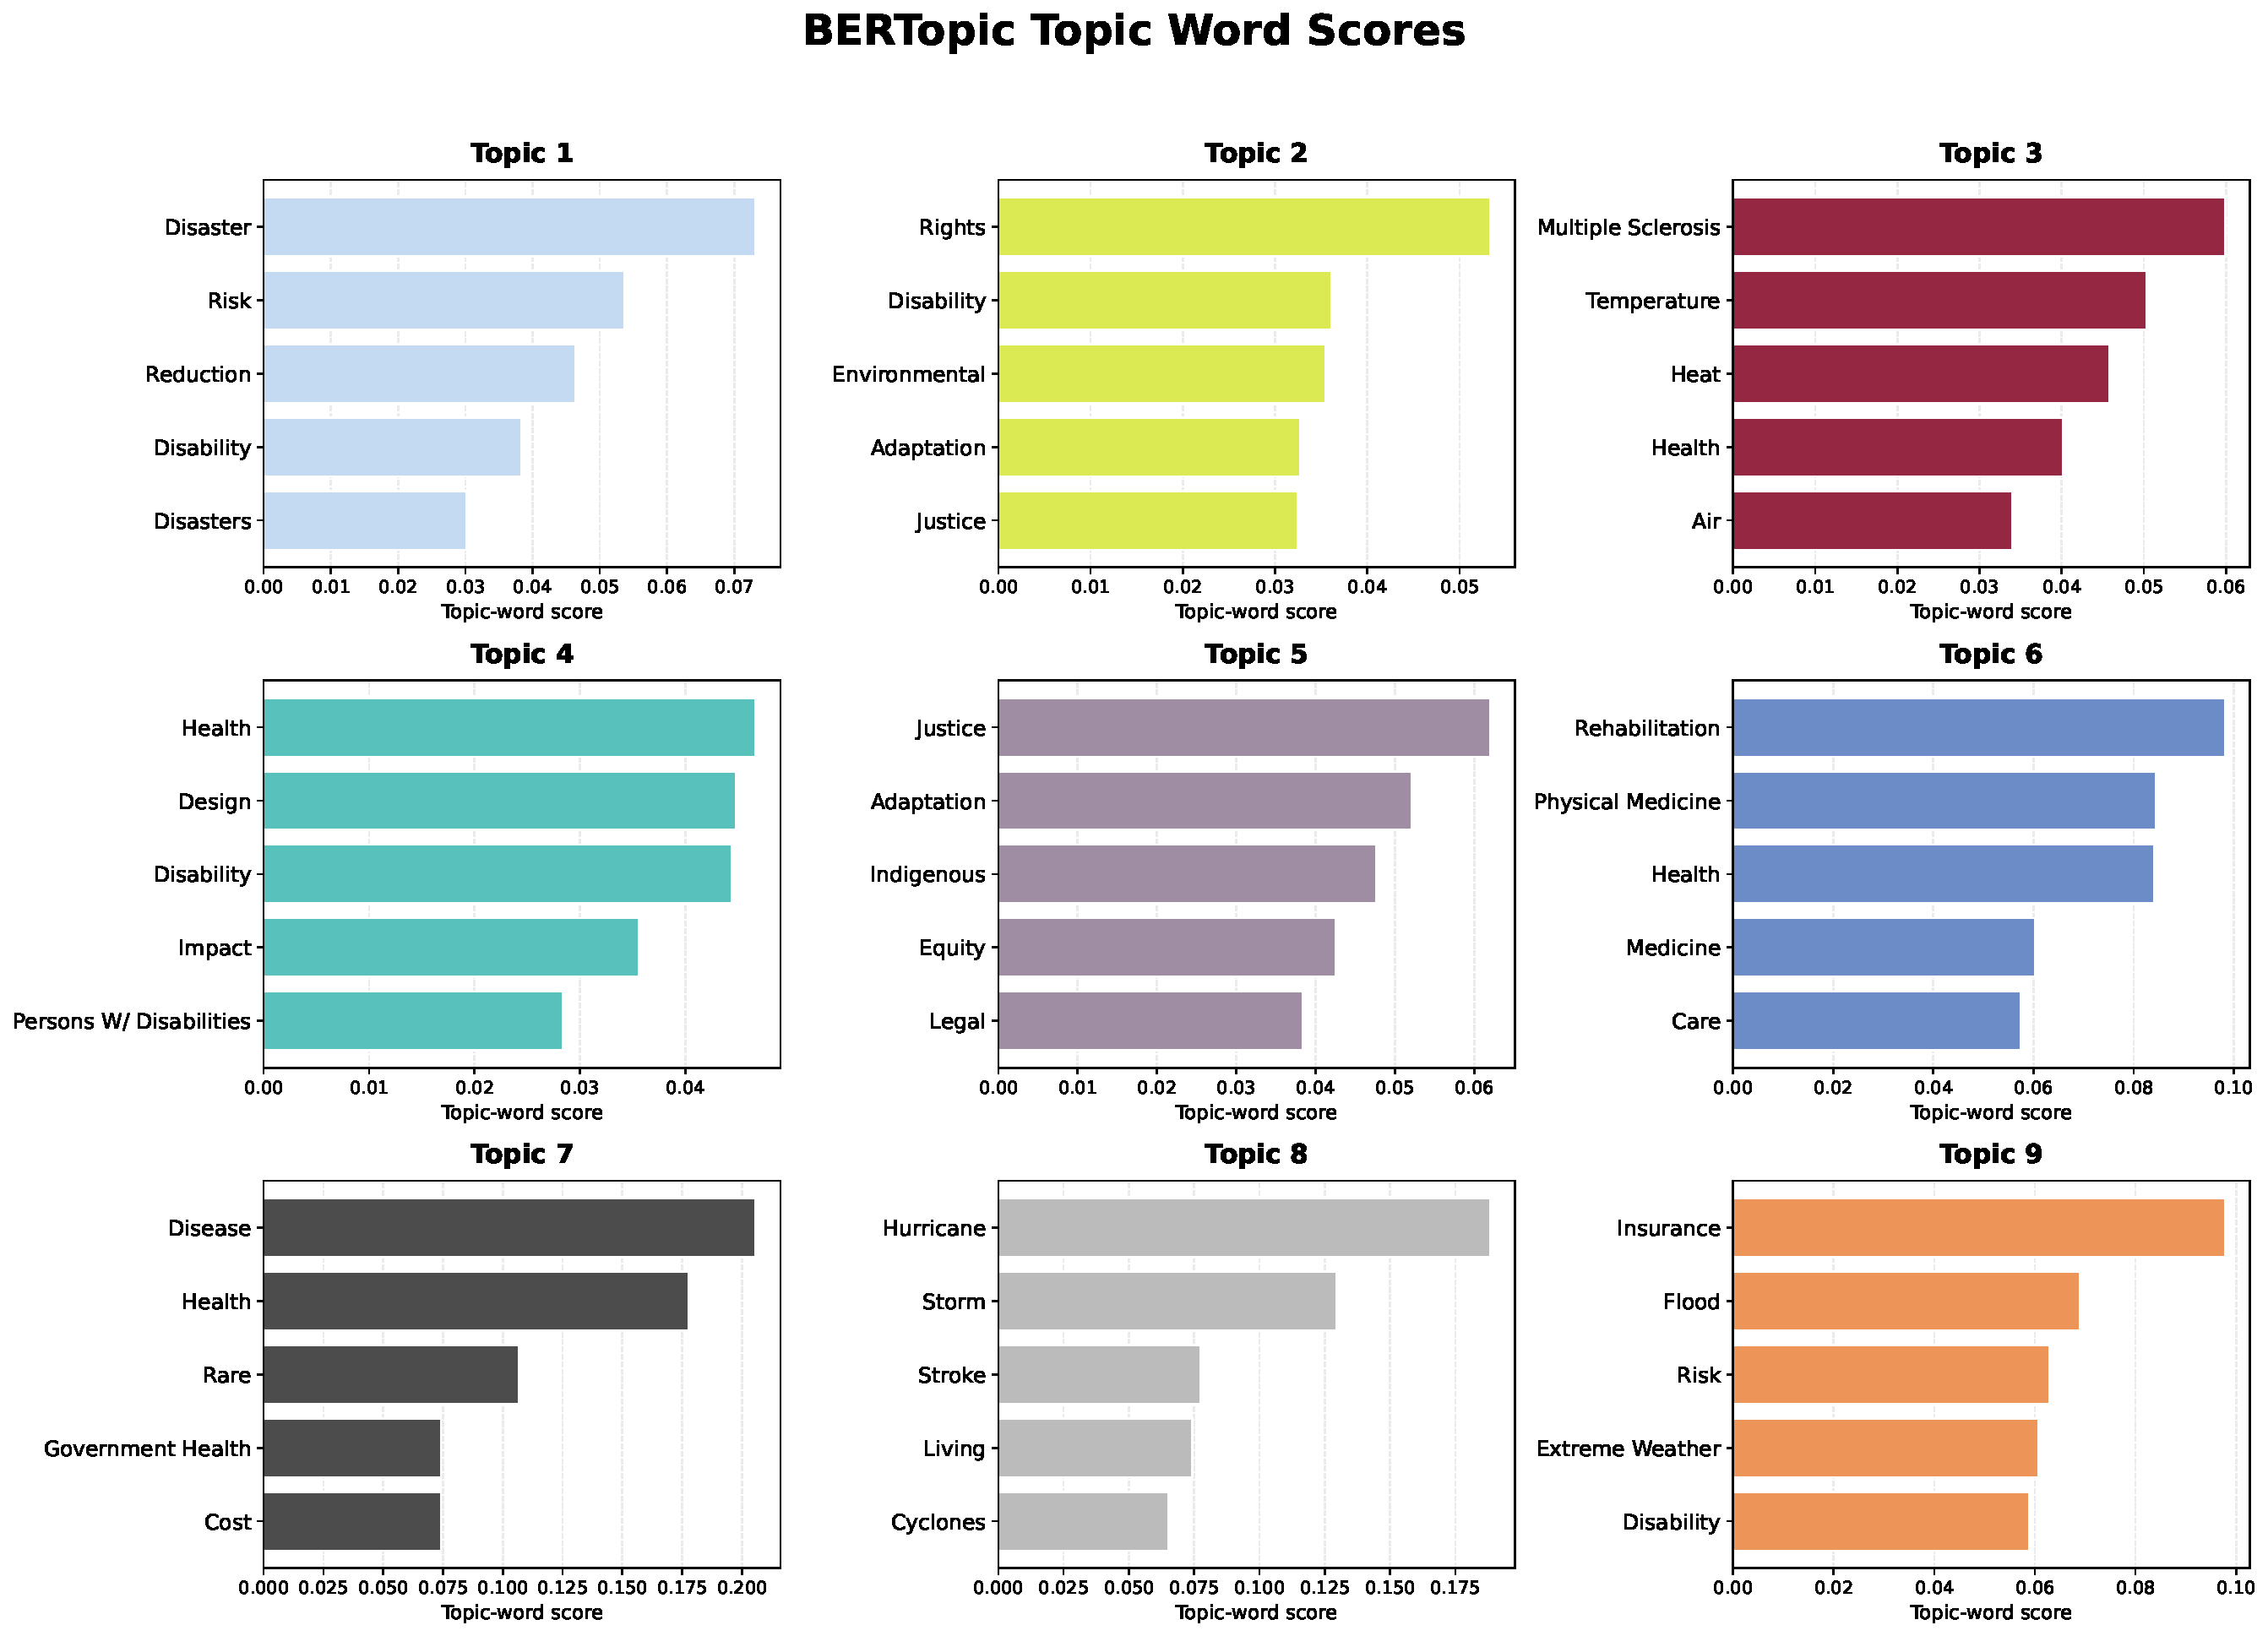
\includegraphics[width=\textwidth]{bertopic_barchart_267_cleaned.pdf}
  \caption{Top representative terms per BERTopic topic, ranked by class-based TF-IDF score.}
  \label{fig:bertopic_barchart}
\end{figure}

In summary, terms that are sharply concentrated in a single topic (\textit{disaster}, \textit{rehabilitation}, \textit{hurricane}, \textit{insurance}) mark the field's stable thematic cores, while terms that recur across several topics with overlapping weight (\textit{adaptation}, \textit{justice}, \textit{rights}, \textit{equity}, \textit{environmental}, \textit{inclusive}) mark an evolving rights and adaptation discourse in which conceptual boundaries are still being negotiated.

\subsection{Topic prevalence over time}
Figure~\ref{fig:bertopic_topics_over_time} disaggregates the publication trend by topic, showing the prevalence of each BERTopic cluster across years.

\begin{figure}[H]
  \centering
  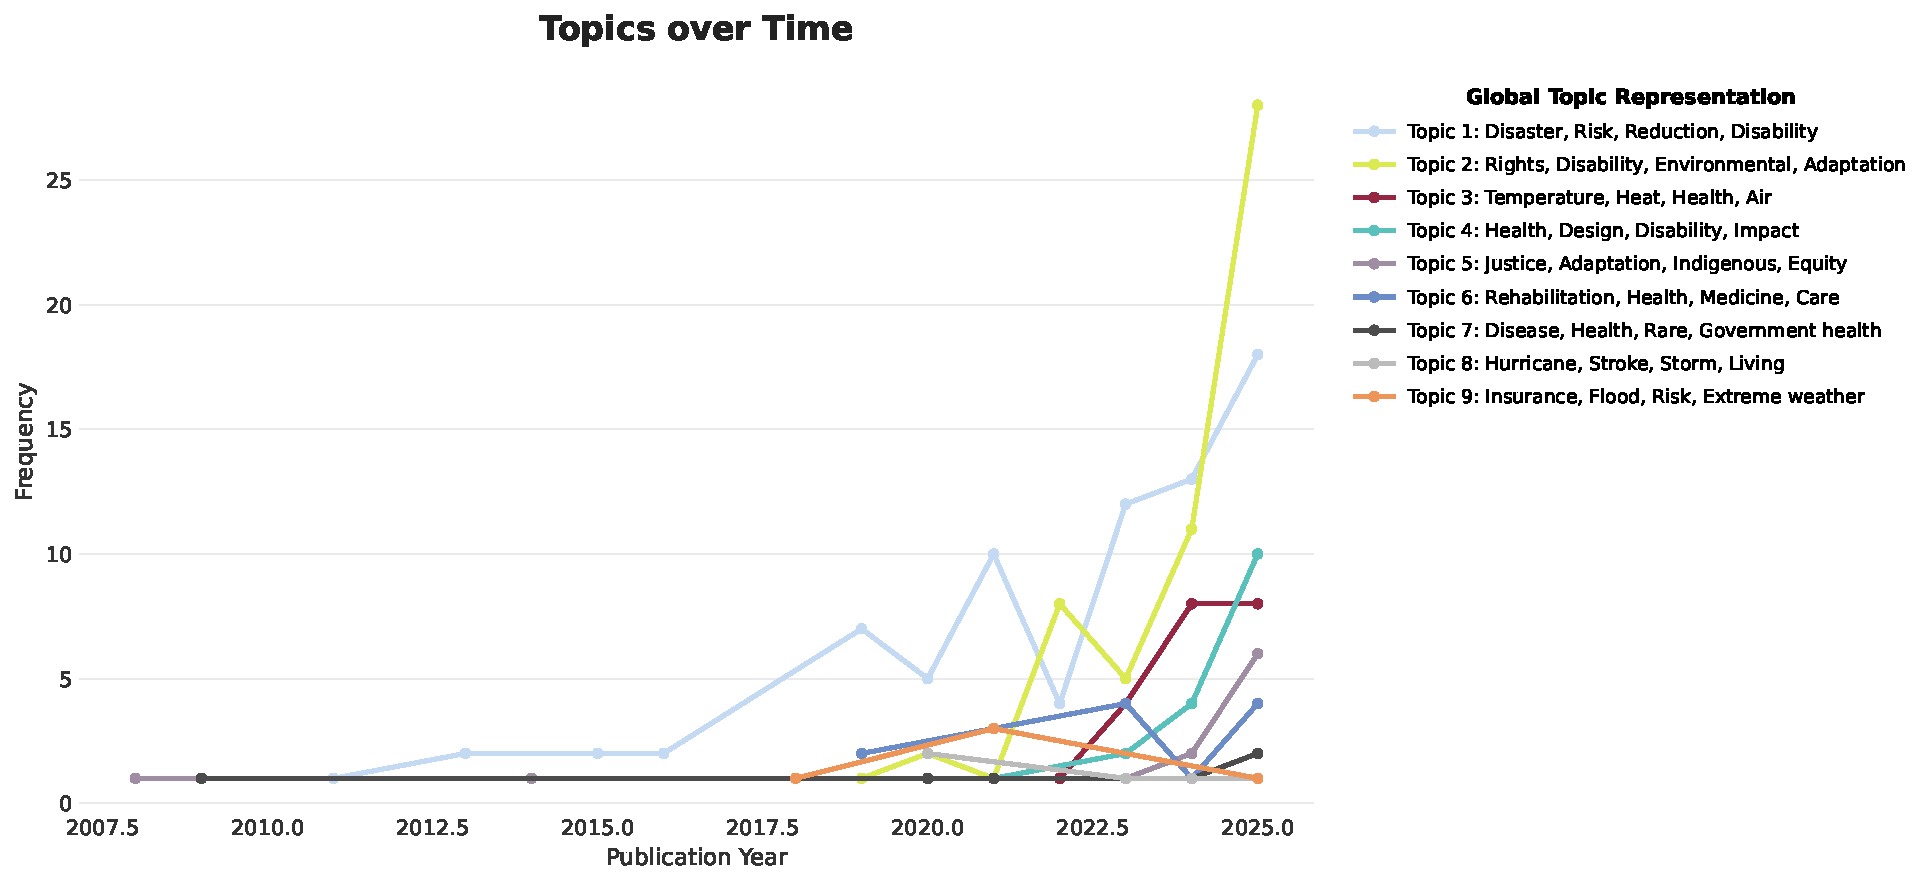
\includegraphics[width=\textwidth]{bertopic_topics_over_time.pdf}
  \caption{Topic prevalence over time across the nine BERTopic clusters.}
  \label{fig:bertopic_topics_over_time}
\end{figure}

The chart reinforces the pattern in the overlay analysis (Section~4.3.2): most topics show little or no activity before 2019 and a substantial increase from 2020 onwards. The two dominant clusters, Topic~1 (disaster risk and risk reduction) and Topic~2 (rights, environmental justice and adaptation), account for most of the post-2020 expansion, while the smaller hazard- and disease-specific clusters (Topics 7--9) remain low and intermittent, corresponding to specialised sub-literatures rather than growing thematic strands. The field is moving from a narrower disaster-risk framing towards adaptation-, justice- and rights-oriented framings, while behavioural and policy-evaluation themes remain absent from the most active clusters.

\subsection{Annual publication trend of the topic-modelling corpus}
Figure~\ref{fig:bertopic_year} reports the annual publication volume of the 211 records included in the topic modelling stage, without disaggregation by topic. Of the 267 records in the extended dataset, 56 fall into topic~$-1$, BERTopic's outlier label for documents HDBSCAN could not assign to any cluster \cite{mcinnes2017hdbscan}, leaving 211 across the nine substantive topics. These outliers are excluded from the labelled topics but retained in the dataset totals. The aggregate trend is consistent with the chart above: activity is low before 2019, increases steadily from 2020, and accelerates in 2024--2025, matching the broader expansion of climate research and the growing visibility of disability as an analytical category within it \cite{kosanic2022inclusive,stein2022disability}. Two caveats apply. Database coverage lags publication, so the 2025 figure is partial and should be treated as a lower bound; and because the corpus has been pre-filtered through the screening process described in Section~4.2.2, the trend reflects records retained for review rather than overall publication activity in the field.

\begin{figure}[H]
  \centering
  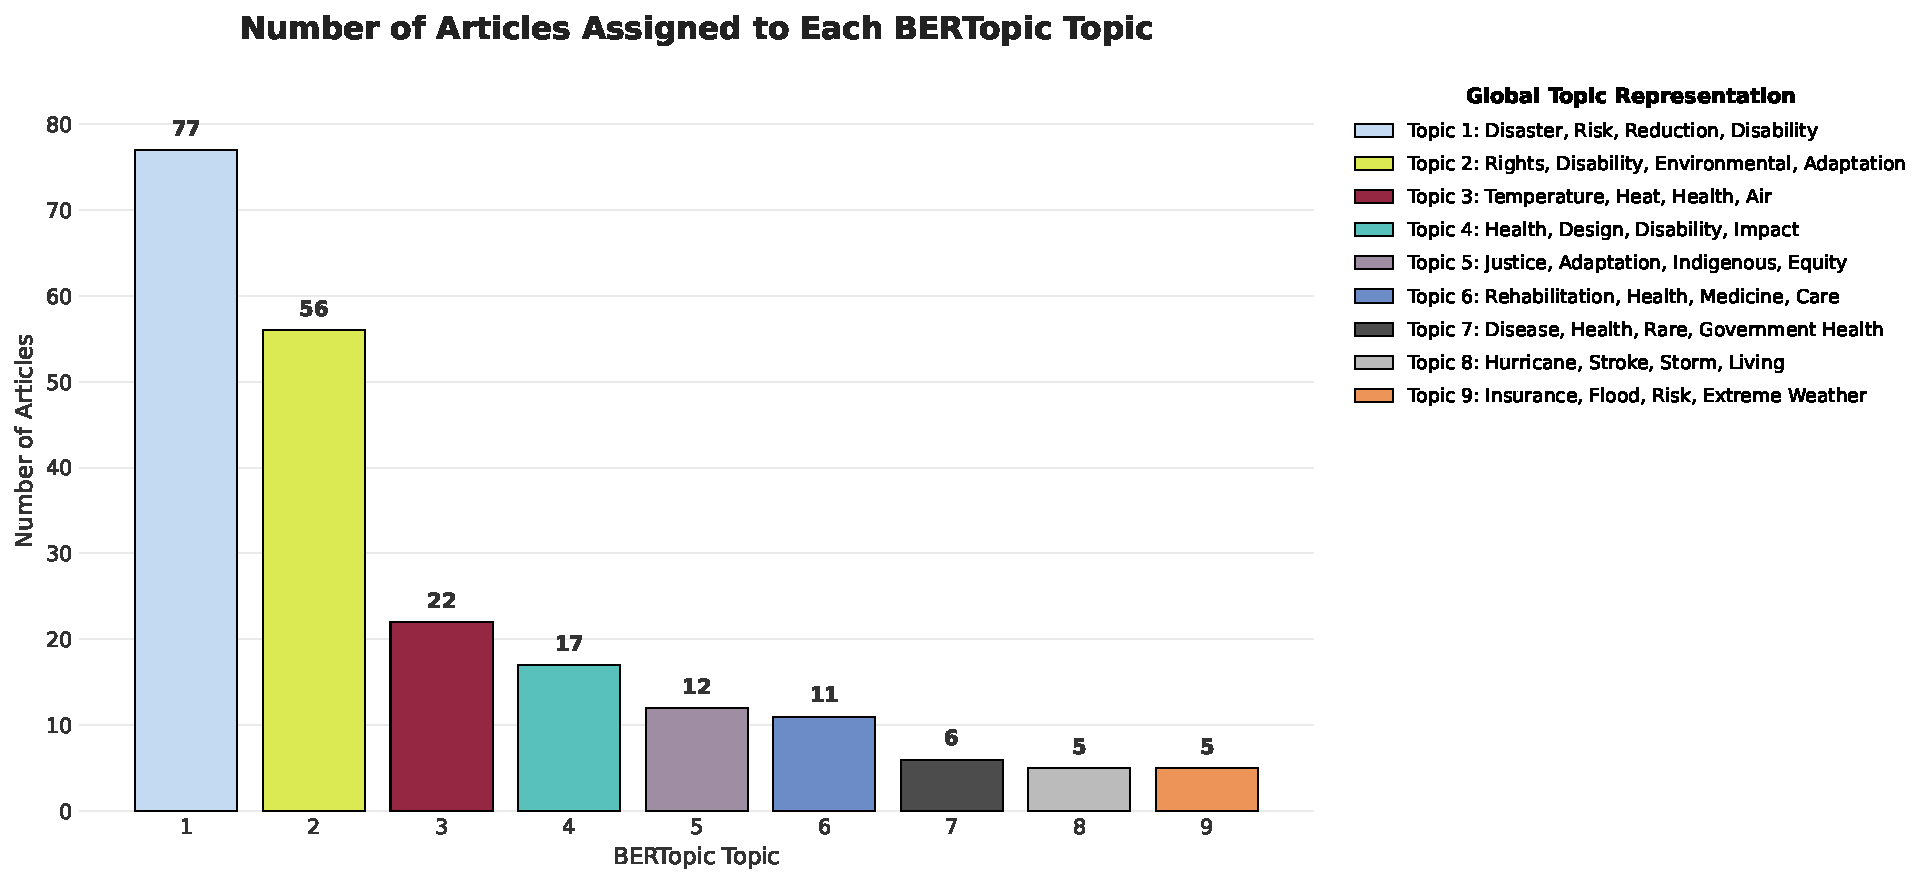
\includegraphics[width=\textwidth]{bertopic_year.pdf}
  \caption{Annual publication volume of records included in the BERTopic analysis (n=211).}
  \label{fig:bertopic_year}
\end{figure}





\subsection{Summary of the topic modelling analysis}
Overall, the BERTopic analysis confirms that the literature clusters around disaster risk reduction, rights and environmental justice, and environmental health, with the rights and justice topics driving most of the recent growth. Participation, agency, behavioural response, policy evaluation and computational policy tools do not appear as topics in their own right, a structural absence that motivates the methodological direction developed in the remainder of this thesis.


\section{Qualitative Synthesis}
The bibliometric and TM analyses in Sections~4.3 and~4.4 mapped the structure of the wider literature; this section interrogates how disabled people are positioned during social behaviours within climate governance through a close reading of the 42-record core dataset assembled from the 267-record extended dataset (Section~4.2.2). The synthesis is thematic rather than statistical: it identifies recurring conceptual moves, isolates where they break down in practice, and uses those breakdowns to characterise the behavioural and institutional mechanisms through which exclusion is reproduced.

\subsection{Approach}
\label{sec:4-5-1-approach}
The bibliometric analysis (Section~4.3) and the topic modelling (Section~4.4) together show that the literature is anchored in disaster risk, rights and adaptation, that it now recognises disability at the level of policy text, and that participation, behavioural response and policy evaluation persist as structural absences rather than developed strands. Therefore, this synthesis focuses specifically on the recognition to implementation problem: how, and at which points, the formal recognition of disability in climate governance is, or is not, carried through into operational, behaviourally grounded adaptation practice. This focusing converts a structural gap into a screening direction for the core dataset.

\textbf{Main review question.} \emph{How, and to what extent, does the disability and climate adaptation literature translate the formal recognition of disability into operationally meaningful and behaviourally informed climate adaptation governance?}

Records from the 267-record extended dataset were retained only where they carried behavioural evidence relevant to at least one of four stages of the recognition to implementation pathway:

\begin{itemize}
    \item \textbf{Recognition and framing.} How is disability framed, and do disabled people internalise, accept or contest dominant vulnerability framings?
    \item \textbf{Participation and representation.} How do disabled people and disability-led organisations behave in participatory processes, and how do state and emergency actors respond?
    \item \textbf{Adaptive behavioural response.} What adaptive behaviours do disabled people exhibit in response to climate stress?
    \item \textbf{Institutional implementation.} How do institutional and policy actors behave when translating recognition of disability into operational adaptation practice?
\end{itemize}

Coding followed a hybrid, deductive-led thematic approach combining an a priori framework with inductively generated codes \cite{fereday2006demonstrating,azungah2018qualitative}. A code manual was first developed deductively from the review question, the four behavioural sub-questions and the theoretical anchors, specifying four predefined categories, behaviours, framings, evidence types and policy claims, each defined against the recognition-to-implementation pathway. The template was piloted on a small set of records to refine these definitions, then applied to all 42 core records, which were read in full and coded manually, with inductive codes added where material fell outside the categories. As the sole coder, I checked stability by re-coding a subset after an interval. Coded passages were collated within each category and connected across records to surface recurring behavioural moves, which were refined inductively into the patterns of exclusion reported in Section \ref{sec:patterns}; their number was not fixed in advance. Finally, the patterns were corroborated against the source records to confirm they were grounded in the data rather than imposed by the framework.


\subsection{Findings}
\textbf{Recognition without implementation.} Disability is widely acknowledged in formal climate and disaster policy yet remains operationally weak. Policy document analyses in Nepal \cite{devkota2023nepal}, Indonesia \cite{pertiwi2020indonesia}, Bangladesh \cite{islam2015bangladesh}, Zimbabwe \cite{lunga2019zimbabwe}, India \cite{hiranandani2015india}, Taiwan \cite{lee2019taiwan}, Massachusetts \cite{brown2025massachusetts} and the FEMA Region 9 jurisdictions \cite{gershon2021fema} all report the same gap, and the five-year global review of the Sendai Framework reaches the same conclusion at international scale \cite{bennettgayle2020sendai}.

\textbf{Vulnerability framing and its contestation.} A large share of the corpus positions disabled people primarily through a vulnerability frame, constructing them as recipients of protection rather than as decision-makers or knowledge holders \cite{sheknoble2023communicating,pertiwi2020indonesia,tagalo2020davao}. The framing is no longer uncontested: a coherent strand of recent critical disability studies and intersectional and decolonial scholarship deliberately sets out to displace it \cite{stjernholm2025critical,setijaningrum2024tokenism,pirmasari2023halinai,eriksen2025rock}.

\textbf{Participation as DPO leadership.} Meaningful participation is overwhelmingly led by DPOs rather than achieved through mainstream inclusion programmes. The Indonesian DPO case studies \cite{pertiwi2019dpo,pertiwi2022bridging,villeneuve2017dpo}, the Vietnam capability approach work \cite{ton2021agency,ton2020capabilities}, the Deaf twin track literature \cite{craig2023twintrack,cooper2021vietnam,calgaro2021silent} and the Yogyakarta partnership analysis \cite{rahatiningtyas2025yogyakarta} all converge on this point: state and emergency management actors lack the partnership architecture required to engage disability led actors effectively \cite{twigg2014attitude,ewen2025nepal}.

\textbf{Behavioural evidence: present but not policy coupled.} The corpus contains substantial qualitative evidence on disabled people's responses to climate stress through capability approach studies in Vietnam and Assam \cite{ton2020capabilities,ton2021agency,doll2025assam}, Person Centred Emergency Preparedness work in Australia \cite{villeneuve2021pcep,crapis2024australian}, Queensland cyclone interviews \cite{quaill2019queensland}, the Vanuatu Cyclone Pam evaluation \cite{webb2020vanuatu}, disability inclusive survey work with over four hundred respondents \cite{skaggs2025data} and the Tuvalu and Cambodia lived experience studies \cite{elisala2020tuvalu,gartrell2020cambodia}. What is missing is more specific: evidence that is comparable across contexts, tied to particular policy options and structured for computational policy evaluation. The limitation is architectural rather than informational.

\textbf{Climate adaptation governance, narrowly defined, is a smaller literature.} Most of the corpus addresses disaster risk reduction under the Sendai Framework, and most climate-relevant insight has been imported through shared hazard categories such as floods, cyclones and heatwaves. Papers that engage climate adaptation governance directly remain few in number and recent in date \cite{brown2025massachusetts,engelman2025california,eriksen2025rock,duke2025climatecourts,pirmasari2023halinai,alexander2025climatedisability,campbell2023rehabilitation,eaton2022mental,alexander2021daytomorrow}, which shows that the sub-field is emerging rather than saturated and justifies methodological development rather than further mapping.

\subsection{Behavioural patterns of exclusion}
\label{sec:patterns}
Read across the five findings, four recurrent behavioural patterns emerge through which exclusion is reproduced: vulnerability framing, internalised acceptance of token inclusion, DPO led participation, and institutional normalisation. They are summarised in Table~\ref{tab:behavioural-patterns}; the social science frameworks that help explain them are introduced in Section~\ref{sec:mechanisms}.

\begin{table}[H]
\centering
\small
\renewcommand{\arraystretch}{1.3}
\caption{Behavioural patterns of exclusion identified in the core dataset}
\label{tab:behavioural-patterns}
\begin{tabularx}{\textwidth}{>{\raggedright\arraybackslash}p{0.24\textwidth} >{\raggedright\arraybackslash}X >{\raggedright\arraybackslash}p{0.26\textwidth}}
\toprule
\textbf{Pattern} & \textbf{Observed behaviour} & \textbf{Key references} \\
\midrule
Vulnerability framing
& Disabled people positioned primarily as recipients of protection rather than as decision makers, naturalising their exclusion from policy processes.
& \cite{sheknoble2023communicating,pertiwi2020indonesia,tagalo2020davao,stjernholm2025critical} \\
\midrule
Internalised acceptance of token inclusion
& Muted demand for operational reform once formal recognition is achieved; acceptance of token participation in structures disabled stakeholders did not design.
& \cite{setijaningrum2024tokenism,tagalo2020davao,bennettgayle2020sendai} \\
\midrule
DPO led participation
& Meaningful participation only where DPOs lead, not where they are consulted; depends on trusted communication and partnership architecture.
& \cite{pertiwi2019dpo,villeneuve2017dpo,ton2021agency,craig2023twintrack,rahatiningtyas2025yogyakarta} \\
\midrule
Institutional normalisation
& Climate and disaster systems assume able bodied users; assumptions embedded in routine planning even where no discrimination is intended.
& \cite{lunga2019zimbabwe,brown2025massachusetts,gershon2021fema,ivey2014deafhh,engelman2025california} \\
\bottomrule
\end{tabularx}
\end{table}

\subsection{Summary}
The synthesis shows that the recognition--implementation gap repeatedly flagged in Sections~4.3 and~4.4 is not a passive absence of evidence but the product of identifiable behavioural mechanisms of exclusion. Four such mechanisms emerge consistently from the 42-record core dataset, vulnerability framing, internalised acceptance of token inclusion, DPO led participation against weak partnership architecture, and institutional normalisation of able bodied assumptions, and are summarised in Table~\ref{tab:behavioural-patterns}. Their visibility in the corpus is what makes the gap analytically tractable: once exclusion is read as the outcome of specific, repeatable behaviours rather than as a diffuse normative shortfall, it becomes possible to explain why the gap persists and to design methodological tools that act on those mechanisms directly. Section~\ref{sec:mechanisms} interprets these four patterns through established social science frameworks, turning the recognition--implementation gap from a descriptive problem into one that can be operationally addressed.



\section{Social Behavioural Mechanisms Identified}
\label{sec:mechanisms}
This section interprets the four behavioural patterns identified in Section~\ref{sec:patterns} through established social science frameworks. The aim is not to test the frameworks empirically but to use them as analytic lenses that explain why the patterns persist and that inform the design choices developed later in the thesis. The mapping between patterns and frameworks is summarised in Table~\ref{tab:mechanism-theory}.

The \textbf{capability approach} evaluates wellbeing and agency in terms of what people can do and be given the resources available and the institutional conversion factors that translate them into functioning \cite{sen_1999_development,nussbaum_2011_capabilities}; the corpus uses it directly to explain why DPO led participation succeeds where mainstream programmes do not \cite{ton2021agency,villeneuve2021pcep,doll2025assam}. \textbf{Critical disability studies and the social model} argue that disability is produced by environmental and institutional barriers rather than impairment alone, so the apparent vulnerability of disabled people is itself a product of ableist design \cite{oliver_1990_politics,stjernholm2025critical,setijaningrum2024tokenism}. \textbf{System justification theory} describes the tendency of disadvantaged groups to treat unequal arrangements as natural and legitimate \cite{jost_2003_decade,Akike2025}, which helps account for the unusual stability of the recognition and implementation gap and the acceptance of token participation. \textbf{Social dominance theory} describes how societies sustain group based hierarchies through legitimising narratives \cite{sidanius_pratto_1999_socdom,Murcott2025,Harpur2025}: reading the vulnerability frame as such a narrative makes its persistence intelligible. \textbf{Institutional theory} explains how organisational routines reproduce embedded assumptions through habit, mimicry and normative pressure rather than explicit decisions \cite{dimaggio_powell_1983_ironcage}, accounting for the institutional normalisation pattern in which planning routines reproduce able bodied assumptions \cite{brown2025massachusetts,gershon2021fema,lunga2019zimbabwe}.

\begin{table}[H]
\centering
\small
\renewcommand{\arraystretch}{1.3}
\caption{Mapping between behavioural patterns and social behavioural frameworks}
\label{tab:mechanism-theory}
\begin{tabularx}{\textwidth}{>{\raggedright\arraybackslash}p{0.22\textwidth} >{\raggedright\arraybackslash}p{0.22\textwidth} >{\raggedright\arraybackslash}X}
\toprule
\textbf{Behavioural pattern} & \textbf{Primary framework} & \textbf{How the framework accounts for the pattern} \\
\midrule
Vulnerability framing
& Social dominance theory; critical disability studies
& Vulnerability functions as a legitimising narrative that allows institutions to treat exclusion as protection, which critical disability studies reframes as an ableist construction \cite{sidanius_pratto_1999_socdom,Murcott2025,oliver_1990_politics,stjernholm2025critical}. \\
\midrule
Internalised acceptance of token inclusion
& System justification theory
& Disadvantaged group members treat unequal arrangements as natural, dampening demand for reform and enabling token participation to substitute for substantive change \cite{jost_2003_decade,Akike2025,setijaningrum2024tokenism}. \\
\midrule
DPO led participation
& Capability approach
& DPOs supply the conversion factors, trusted channels and partnership architecture that translate formal entitlements into actual functioning \cite{sen_1999_development,ton2021agency,villeneuve2021pcep,rahatiningtyas2025yogyakarta}. \\
\midrule
Institutional normalisation
& Institutional theory
& Organisational routines reproduce embedded able bodied assumptions through habit and normative pressure rather than through explicit discrimination \cite{dimaggio_powell_1983_ironcage,brown2025massachusetts,gershon2021fema,lunga2019zimbabwe}. \\
\bottomrule
\end{tabularx}
\end{table}

\subsection{Implications for narrative design}
\label{sec:4-6-1-narrative-design-implications}
The mapping in Table~\ref{tab:mechanism-theory} carries direct implications for the design of the empirical method that follows in the next chapter. If exclusion is reproduced through identifiable behavioural mechanisms, vulnerability framing carried as a legitimising narrative, internalised acceptance of token participation, DPO mediated conversion factors and institutional routines that normalise able bodied assumptions, then a method intended to generate evidence on those mechanisms must place behaviour, framing and participation architecture at the centre of its design rather than treating them as background variables. Three narrative design implications follow.

Three design principles follow, each tied to one of the behavioural mechanisms. The design should be \emph{capability oriented}, exposing the conversion factors, information, communication, trusted intermediaries, accessible environments, that translate formal entitlements into actual functioning \cite{sen_1999_development,ton2021agency,villeneuve2021pcep}. It should treat \emph{vulnerability framing as a choice rather than a default}, so that its acceptance or contestation becomes observable in the narrative itself \cite{stjernholm2025critical,jost_2003_decade,setijaningrum2024tokenism}. And it should embed \emph{participation architecture as structural}, with DPO mediated channels, twin track communication and disability led decision routes built into the scenario rather than bolted on as accommodations \cite{pertiwi2019dpo,villeneuve2017dpo,craig2023twintrack,rahatiningtyas2025yogyakarta}.

Table~\ref{tab:narrative-design-instructions} consolidates this argument by pairing each of the four behavioural mechanisms identified in Section~\ref{sec:patterns} with the design principle and the concrete narrative design instruction it implies.

\begin{table}[H]
\centering
\small
\renewcommand{\arraystretch}{1.3}
\caption{Behavioural mechanisms and corresponding narrative design instructions}
\label{tab:narrative-design-instructions}
\begin{tabularx}{\textwidth}{>{\raggedright\arraybackslash}p{0.20\textwidth} >{\raggedright\arraybackslash}p{0.22\textwidth} >{\raggedright\arraybackslash}X}
\toprule
\textbf{Behavioural mechanism} & \textbf{Design principle} & \textbf{Concrete narrative design instruction} \\
\midrule
Vulnerability framing
& Framing as a choice, not a default
& Provide decision points at which the same disabled character can be positioned as recipient of protection or as decision-maker, so the legitimising work of the vulnerability frame, and its acceptance or contestation, becomes observable inside the narrative \cite{stjernholm2025critical,sidanius_pratto_1999_socdom}. \\
\midrule
Internalised acceptance of token inclusion
& Substantive participation routes alongside symbolic ones
& Offer parallel narrative routes, consultative or token participation versus disabled led decision-making, and let players accept, decline or reconfigure the token route, rendering the muting effect of system justification visible rather than assumed \cite{jost_2003_decade,setijaningrum2024tokenism}. \\
\midrule
DPO led participation
& Participation architecture as structural
& Embed DPO mediated channels, twin track communication and disability led decision routes as designed features of the scenario rather than as accessibility add-ons, so meaningful participation can occur on the same terms it does in the corpus \cite{pertiwi2019dpo,villeneuve2017dpo,craig2023twintrack,rahatiningtyas2025yogyakarta}. \\
\midrule
Institutional normalisation
& Capability oriented scenarios that expose institutional routines
& Build scenarios around the conversion factors, information, communication, accessible environments, trusted intermediaries, so able bodied institutional routines appear as objects of action rather than as invisible background, allowing players to act on or against them \cite{sen_1999_development,ton2021agency,villeneuve2021pcep,brown2025massachusetts}. \\
\bottomrule
\end{tabularx}
\end{table}

Taken together, these implications establish the plausibility of a narrative based design as a response to the gap: the behavioural patterns the literature review identifies are exactly the patterns a narrative method is well placed to elicit, because they manifest as situated decisions and framings rather than as latent attitudes that survey or interview methods can only recover partially. Section~\ref{sec:mechanisms} is therefore not only an interpretive aid but the analytic warrant for the design developed in the following chapter.


\section{Discussion}
The three analytical lenses converge rather than producing competing readings. The bibliometric and topic modelling work shows a field dominated by disaster risk reduction and growing fastest in rights and environmental justice, with no recognisable cluster around participation, agency, behavioural response or policy evaluation. The qualitative synthesis identifies the same gap from the demand side: disability is recognised in policy text yet implementation is consistently weak, meaningful participation occurs only where DPOs lead, and behavioural evidence on adaptive choices is rich but not structured for policy use. Read against the patterns in Section~\ref{sec:patterns} and the framework mapping in Section~\ref{sec:mechanisms}, these gaps are the predictable output of identifiable behavioural mechanisms, and Section~\ref{sec:4-6-1-narrative-design-implications} translates that mapping into the design specification the next chapter develops.

Two limitations qualify the review, but each is bounded in its likely effect on the behavioural conclusions. Grey and disability led literature is under indexed in mainstream databases, yet by its nature this literature tends to amplify rather than contradict the DPO led participation and frame contestation patterns. The critical, intersectional and decolonial turn rests on a small but growing literature and should be read as directional rather than settled \cite{stjernholm2025critical,eriksen2025rock,setijaningrum2024tokenism}; its growth direction is consistent with the patterns identified, so additional work in this strand is more likely to reinforce the conclusions than to reverse them. The probability that deeper or more peripheral literature would materially overturn the recognition - implementation gap or the four mechanisms is therefore low.

The chapter's behavioural conclusions can therefore be treated as robust. What follows in the rest of the report is the methodological response to the gap they identify, developed in Section~\ref{sec:4-6-1-narrative-design-implications} and the chapters that follow, rather than a compensation for the review's limitations.


%\section{Pilot Study}
%\subsection{Purpose of the Pilot Study}
%The pilot study will test the feasibility of using a serious narrative game as a participatory research method for disability-inclusive climate adaptation policy evaluation. Its purpose is not to produce final generalisable findings, but to examine whether the proposed game-based method can generate meaningful behavioural and narrative data from disabled participants.

%The pilot will have four main aims. First, it will assess whether climate adaptation scenarios can be translated into accessible and understandable game situations. Second, it will examine whether participants’ in-game choices and reflections can reveal adaptive strategies, perceived barriers and policy responses. Third, it will test whether the game interface and interaction methods are accessible for participants with different needs. Fourth, it will provide preliminary data that can inform the later Grounded Theory, Topic Modelling and Agent-Based Modelling stages.

%In this sense, the pilot study functions as a proof of concept. It will help refine the game design, data collection protocol and analytical framework before the full empirical study is conducted.
%\subsection{Case Study Context}
%The initial case study is expected to focus on climate adaptation scenarios relevant to urban and community contexts. The specific geographical setting will be refined after further discussion with supervisors and potential collaborators. At this stage, China is considered a possible initial context because of its relevance to accessibility construction, rapid urban development, climate adaptation needs and the researcher’s intended impact pathway.

%However, the pilot study will not assume that one national or urban context can represent all disability experiences. Instead, the case study will be used to develop and test a methodological framework that can later be adapted to different contexts. The purpose is to examine how disability-related barriers, climate risks and policy decisions interact within a structured scenario environment.

%The selected scenarios will therefore focus on situations where climate adaptation policies directly affect disabled people’s access to safety, resources, information and participation. These may include heatwave response, flood evacuation, emergency communication, transport disruption, access to shelters, and the use of assistive technologies during climate-related events.
%\subsection{Serious Narrative Game Concept}
%The serious narrative game will be designed as an interactive scenario-based environment. Participants will be presented with climate-related situations and asked to make decisions under different policy, resource and accessibility conditions. The game will combine narrative storytelling with structured decision points, allowing players to express both what they choose and why they choose it.

%The game is not designed simply to teach participants about climate change. Instead, it is designed to elicit decision-making processes, adaptive behaviours and policy perceptions. For example, a player may need to decide whether to follow official evacuation advice, rely on informal support networks, seek accessible transport, stay at home, or use alternative resources. Each decision can reveal how participants understand risk, trust institutions, evaluate accessibility and respond to constraints.

%The narrative format is important because climate adaptation is not only a matter of rational choice. It is shaped by lived experience, emotion, uncertainty, social support, previous experiences with institutions and perceived fairness. A narrative game can make these dimensions more visible than a conventional survey, while still providing a structured environment for comparison across participants.
%A preliminary visual concept has been developed to explore how climate hazards and disability profiles may be translated into a game interface. As shown in Figure 1, the concept uses a motor disability profile as an example and presents multiple climate-related scenarios, including floods, droughts, cyclones, storms and heat. The storm scenario is further divided into spatial contexts such as home, public buildings and outdoor environments. This structure is intended to support scenario-based decision-making and to generate data on how disabled participants assess risks, resources and accessible adaptation options across different environments.

%\subsection{Scenario Design}
%The pilot game will include a limited number of climate-related scenarios. These scenarios will be selected based on the literature review findings and their relevance to disability-inclusive adaptation.

%Possible scenarios include:
%\begin{enumerate}
   % \item Heatwave and cooling access
% Participants may need to respond to extreme heat while considering accessible transport, cooling centres, medication storage, health needs and social support.
   % \item Flooding and evacuation: Participants may face decisions about evacuation routes, accessible shelters, mobility support, early warning systems and emergency services.
  %  \item Storm or power outage: This scenario may explore dependence on electricity, assistive technologies, communication systems and backup support.
  %  \item Transport disruption: Participants may need to navigate disrupted public transport, inaccessible replacement services or limited mobility assistance.
 %   \item Emergency information access: Participants may respond to different forms of climate warning information, testing whether communication is accessible, timely and trustworthy.
%\end{enumerate}

%Each scenario will include policy levers or institutional responses. These may involve resource allocation, accessible information, transport support, community assistance, emergency planning and participation mechanisms. The aim is to observe how participants respond to different adaptation conditions and where exclusion emerges in practice.
%\subsection{Accessibility and Equity Considerations}
%Accessibility will be central to the pilot study. Since persons with disabilities are not a homogeneous group, the game will need to be adaptable rather than based on a single accessibility solution. The pilot will therefore test whether the interface, language, visual design, audio design and interaction methods are suitable for participants with different access needs.

%The design will be informed by three equity dimensions: distributive, procedural and contextual equity. Distributive equity concerns whether resources and adaptation support are allocated in ways that respond to different disability-related needs. Procedural equity concerns whether disabled people can participate meaningfully in decisions that affect them. Contextual equity concerns whether policies are sensitive to the social, environmental and institutional conditions in which people live.

%These equity dimensions will shape both the game scenarios and the evaluation criteria. For example, a scenario may ask whether accessible shelters are available, whether disabled participants are consulted in planning, or whether emergency information reaches people with different communication needs. In this way, the game will be used to examine not only individual choices, but also the policy conditions that shape those choices.
%\subsection{Data Generated from the Pilot}
%The pilot study is expected to generate several types of data. The first type is behavioural data, including player choices, decision pathways, selected resources, responses to policy options and changes in strategy across scenarios. The second type is narrative data, including written explanations, spoken reflections, post-game interview responses or think-aloud comments. The third type is usability and accessibility feedback, including participants’ comments on the clarity, relevance and accessibility of the game.

%These data will help answer whether the game can capture meaningful adaptive behaviours and policy responses. They will also help identify which variables may later be translated into the ABM. Potential variables include trust in institutions, perceived fairness, access to information, availability of support networks, transport accessibility, resource constraints and willingness to accept or reject policy recommendations.

%The pilot will therefore serve both methodological and substantive purposes. Methodologically, it will test the feasibility of the serious game as a research tool. Substantively, it will provide early insight into how disabled participants interpret and respond to climate adaptation policy scenarios.
%\subsection{Pilot Evaluation Criteria}
%The pilot will be evaluated against several criteria. First, the game should be understandable and accessible to participants. Second, the scenarios should be perceived as relevant to disability-inclusive climate adaptation. Third, the game should generate data that can be analysed through Grounded Theory and Topic Modelling. Fourth, the findings should provide useful inputs for refining ABM agent attributes, decision rules and policy scenarios.

%The pilot will also assess whether participants feel that the game allows them to express their experiences and reasoning. This is important because the aim is not only to collect choices, but also to understand the meanings behind those choices. If the game produces only superficial responses, the design will need to be revised before the full study.
%\subsection{Summary}
%The proposed pilot study will test the central empirical method of the PhD. It will translate findings from the Year 1 review into a serious narrative game that can elicit disabled people’s adaptive behaviours, policy perceptions and responses to climate-related scenarios. The pilot will help refine the game design, accessibility strategy, data collection protocol and ABM variables.

%By functioning as a bridge between literature-based diagnosis and computational policy simulation, the pilot study will play a key role in ensuring that the later ABM is grounded in disability-specific behavioural evidence rather than generic assumptions about adaptation.








%As shown in Figure 6, the topic prevalence chart indicates that the distribution of topics across the corpus is uneven. Disaster risk reduction, emergency preparedness or extreme weather, and climate justice or human rights occupy relatively larger proportions of the dataset. By contrast, health-, heat-, pollution- and demographic-risk topics appear as more specific subthemes. This pattern suggests that the field is not organised around one single dominant concern, but around several partially distinct framings of disability and climate change.
%\begin{figure}[H]
   % \centering
    %\includegraphics[width=0.7\linewidth]%{intertopic_distance_map_recoloured.png}
    %\caption{Intertopic distance map of the six-topic solution}
   % \label{fig:enter-label}
%\end{figure}
%Figure 7 further presents the intertopic distance map of the six-topic solution. Each bubble represents one topic, with bubble size indicating its relative prevalence in the corpus and the distance between bubbles indicating thematic distinctiveness. The map shows that the topics are reasonably separated, suggesting that the six-topic model captures distinguishable thematic areas rather than highly overlapping topics. The distance between the disaster-risk-oriented topic and the justice- or rights-oriented topic is particularly important, as it suggests that these two strands of literature remain thematically distinct.
%\begin{figure}[H]
   % \centering
   % 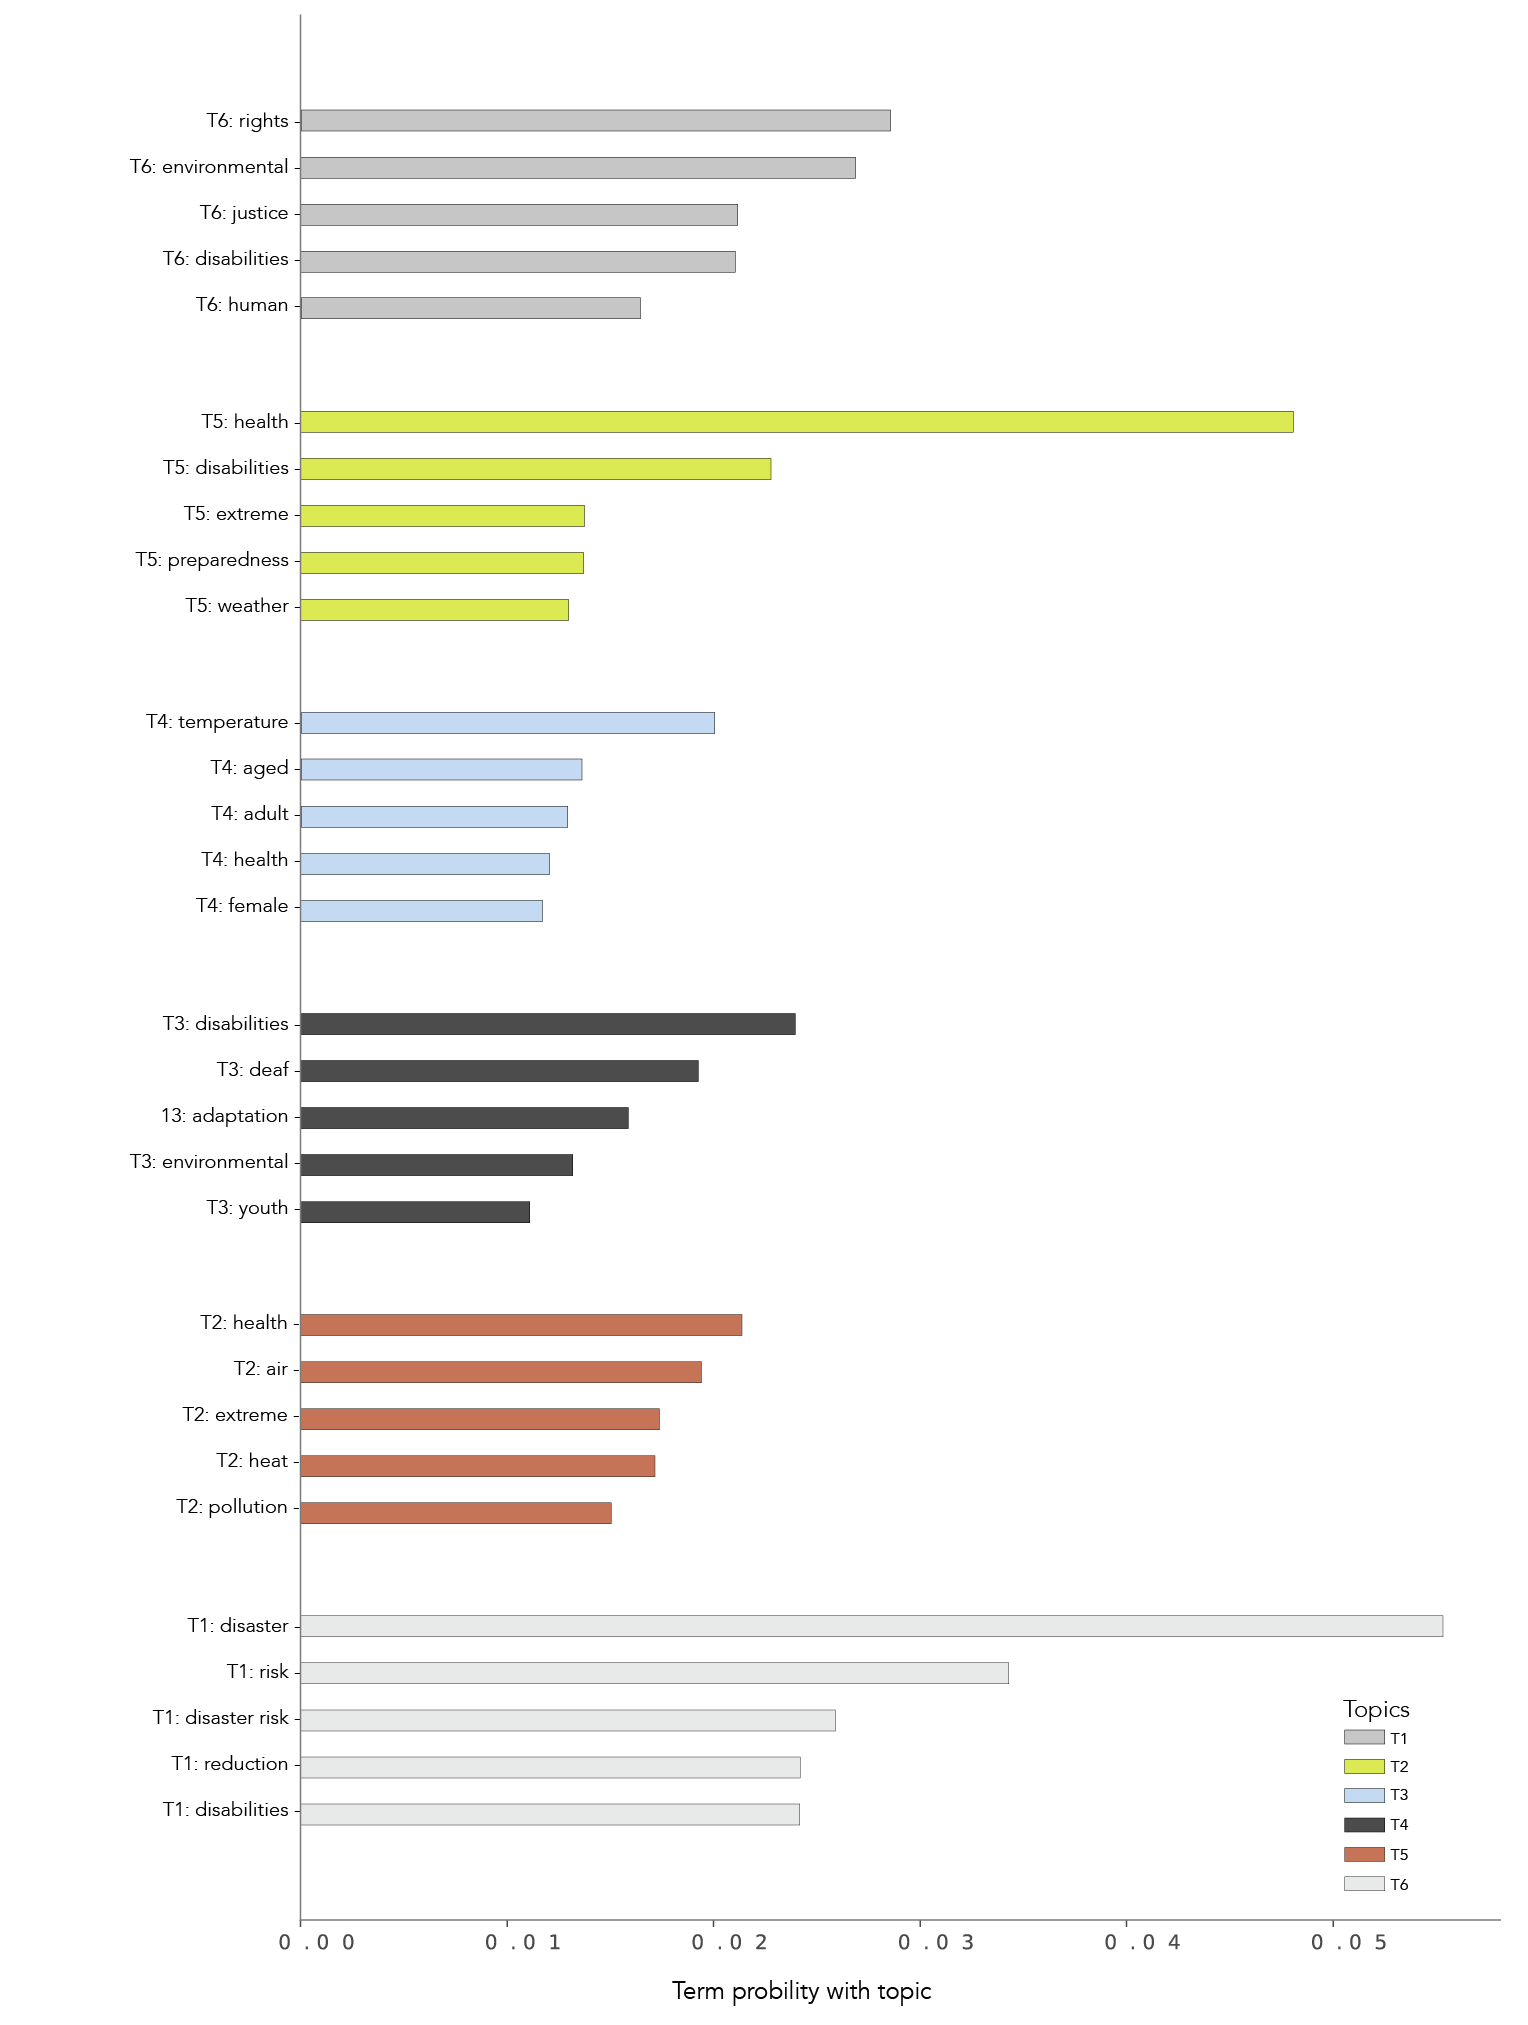
\includegraphics[width=1\linewidth]{TM 2.png}
   % \caption{Topic prevalence across the corpus}
  %  \label{fig:enter-label}
%\end{figure}

%Taken together, the topic modelling results reinforce the bibliometric findings. The literature has made important progress in documenting the vulnerability of persons with disabilities to climate-related hazards, particularly in relation to disaster risk reduction, emergency preparedness, health impacts and environmental exposure. However, the results also reveal a conceptual imbalance. Themes such as participation, agency, behavioural response, policy evaluation, serious games and Agent-Based Modelling do not emerge as central topics. This suggests that existing literature remains more focused on identifying risks and vulnerabilities than on evaluating how disability-inclusive climate adaptation policies work in practice.

%This finding is important for the PhD. It supports the need to move beyond documenting the impacts of climate change on persons with disabilities and towards generating behavioural evidence about how disabled people respond to adaptation policy options. The serious narrative game is therefore proposed as a method for eliciting adaptive strategies, policy perceptions and decision-making processes. These data can then inform the ABM stage, allowing policy scenarios to be evaluated using disability-specific behavioural evidence rather than generic assumptions.


%Second, participation is often mentioned as a normative requirement but is less frequently operationalised as a concrete governance process. Many studies recognise the importance of including persons with disabilities in climate and disaster decision-making, but fewer explain how participation is organised, whether it is accessible, what influence participants have, or how their input changes policy outcomes. This suggests that participation often remains symbolic rather than procedural.

%Third, the literature identifies multiple implementation barriers, including inaccessible information, inadequate emergency planning, limited disability-disaggregated data, inaccessible infrastructure, and weak institutional coordination. However, these barriers are often described as practical problems rather than analysed as part of wider social, behavioural and institutional mechanisms. This limits the ability of existing research to explain why similar forms of exclusion persist despite policy recognition.

%Fourth, there is limited evidence on disabled people’s behavioural responses to adaptation policies. Few studies examine how persons with disabilities assess risk, respond to policy options, trust or distrust institutions, use informal support networks, or make decisions under climate-related constraints. This behavioural evidence gap is important because policy evaluation requires an understanding not only of what policies provide, but also of how people interact with those policies in practice.




%\subsection{Implications for Serious Game Design and ABM Development}

% \begin{table}[htbp]
% \centering
% \footnotesize
% \renewcommand{\arraystretch}{1.35}
% \caption{Translating review findings into game design and ABM development}
% \label{tab:review-findings-game-abm}

% \begin{tabularx}{\textwidth}{
% >{\raggedright\arraybackslash}X
% >{\raggedright\arraybackslash}X
% >{\raggedright\arraybackslash}X
% }
% \toprule
% \textbf{Review finding} & \textbf{Game design implication} & \textbf{Possible ABM implication} \\
% \midrule

% Disability is often framed as vulnerability
% & Design scenarios that foreground choice, agency and strategy
% & Include adaptive behaviour as an agent attribute \\

% Participation is weakly operationalised
% & Include policy consultation and decision-making scenarios
% & Model perceived procedural fairness \\

% Emergency information is often inaccessible
% & Include accessible and inaccessible warning scenarios
% & Add information access as an environmental variable \\

% Resource distribution shapes adaptation
% & Include choices around shelters, transport, health care and assistive technology
% & Model resource availability and allocation \\

% Trust affects policy response
% & Ask participants to respond to institutional advice
% & Include institutional trust as a decision factor \\

% Social support shapes resilience
% & Include formal and informal support options
% & Model support networks as agent-level variables \\

% Policy evaluation is underdeveloped
% & Collect responses to alternative policy scenarios
% & Simulate equity and effectiveness across scenarios \\

% \bottomrule
% \end{tabularx}
% \end{table}
Overall, the Year 1 results provide a clear foundation for the next stages of the PhD. The literature review diagnoses the problem, the narrative game will generate behavioural evidence, and the ABM will translate this evidence into policy simulation. This establishes a coherent pathway from literature-based gap analysis to empirical design and computational policy evaluation.
% \section{Discussion}
% \subsection{Interpretation of Year 1 Findings}
% The first year of the PhD has clarified the conceptual and methodological direction of the research. The original proposal aimed to integrate narrative gaming and Agent-Based Modelling to evaluate climate adaptation policies for persons with disabilities. Through the Year 1 review, this broad aim has been refined into a more specific research pathway: identifying the mechanisms through which disability marginalisation is reproduced in climate governance, using serious narrative gaming to generate disability-specific behavioural evidence, and translating this evidence into ABM-based policy evaluation.

% The bibliometric, topic modelling and scoping review results suggest that existing research has made important progress in recognising disabled people’s disproportionate exposure to climate-related risks. However, the field remains less developed in relation to agency, participation, behavioural response and policy evaluation. This supports the need for a research design that does not only describe vulnerability, but also examines how disabled people respond to adaptation policies and how these responses can inform more inclusive climate governance.
% \subsection{Theoretical Contribution}
% The theoretical contribution of this PhD lies in moving beyond a vulnerability-dominant framing of disability and climate change. While vulnerability remains an important concept for identifying unequal exposure and structural disadvantage, it is insufficient on its own. If disabled people are mainly positioned as vulnerable recipients of protection, their agency, knowledge and role in policy evaluation may be overlooked.

% This PhD therefore reframes disability-inclusive climate adaptation as a problem of participation, behavioural evidence and policy implementation. The Year 1 review shows that exclusion is not only caused by a lack of policy recognition, but also by institutional routines, inaccessible participation, data invisibility and assumptions that treat able-bodied experiences as the norm. By using social-behavioural mechanisms as an analytical focus, the PhD aims to explain why inclusion may remain symbolic even when it is formally acknowledged.

% This theoretical move is important because it connects disability studies, climate governance and behavioural policy research. It positions disability marginalisation not simply as a policy gap, but as a process reproduced through social, institutional and behavioural dynamics.
% \subsection{Methodological Contribution}
% The methodological contribution of the PhD is the integration of literature review, serious narrative gaming, Grounded Theory, Topic Modelling and Agent-Based Modelling into a coherent research framework.

% First, the mixed-methods scoping review combines bibliometric analysis, topic modelling and qualitative synthesis. This provides a more layered understanding of the field than a conventional narrative review alone. Bibliometrics identifies the structure of the literature, topic modelling reveals dominant themes, and scoping synthesis interprets the mechanisms of exclusion in greater depth.

% Second, the serious narrative game is proposed as a participatory method for generating behavioural evidence. Rather than treating games only as tools for education or engagement, this PhD uses narrative gaming as a research environment in which disabled participants can respond to climate-related scenarios, make decisions, and explain their reasoning. This is especially valuable because many existing methods capture policy intentions or general attitudes, but not situated decision-making under climate-related constraints.

% Third, the use of ABM allows the research to translate behavioural evidence into policy simulation. This creates a methodological bridge between individual-level lived experience and system-level policy evaluation. The ABM will not claim to predict reality with certainty; rather, it will function as an exploratory tool for testing how different adaptation policy scenarios may produce more or less equitable outcomes.
% \subsection{Contribution to Inclusive Design and Serious Game Research}
% The PhD also contributes to inclusive design by positioning serious games as more than communication tools. In climate research, games are often used to raise awareness or support scenario learning. In this project, however, the serious narrative game is used to create an accessible and structured space for disabled participants to express adaptive strategies, policy preferences and experiences of exclusion.

% This approach aligns with inclusive design because it treats disabled people as knowledge holders rather than passive users. The game can help make visible how policy designs are experienced in practice: whether information is accessible, whether resources are reachable, whether institutional advice is trusted, and whether participation feels meaningful.

% The pilot study will be important for testing whether this design approach is feasible. It will assess not only whether the game can collect useful data, but also whether the game environment is accessible, understandable and meaningful for disabled participants.
% \subsection{Contribution to Computational Social Science and ABM}
% The proposed ABM stage contributes to computational social science by addressing a common limitation in policy simulation: the use of generic behavioural assumptions. Climate adaptation models often need assumptions about how individuals respond to risk, resources and policy interventions. However, when these assumptions are not informed by disability-specific evidence, they may overlook barriers related to accessibility, trust, support networks and institutional exclusion.

% By using game-generated behavioural data to inform ABM variables and decision rules, this PhD aims to develop a more grounded model of disability-inclusive climate adaptation. Variables such as access to information, transport accessibility, perceived fairness, trust in institutions, social support and adaptive capacity can be informed by participant responses rather than imposed only from top-down assumptions.

% This does not eliminate uncertainty, but it makes the modelling assumptions more transparent and empirically informed. The ABM can then be used to explore how different policy scenarios may affect disabled people differently, and where unintended exclusions may emerge.
% \subsection{Expected Outcomes and Beneficiaries}
% The expected outcomes of the PhD include:
% \begin{enumerate}
%     \item a mixed-methods review paper on disability marginalisation in climate governance;
%     \item a conceptual framework linking exclusion mechanisms, narrative gaming and ABM;
%     \item a serious narrative game prototype for disability-inclusive climate adaptation scenarios;
%     \item a behavioural and narrative dataset generated through game-based participation;
%     \item an ABM framework for evaluating disability-inclusive climate adaptation policy scenarios;
%     \item design and policy recommendations for more equitable adaptation governance.
% \end{enumerate}
% The potential beneficiaries include persons with disabilities, disability organisations, climate adaptation policymakers, urban planners, inclusive design researchers, serious game designers and computational social scientists. The PhD aims to support these stakeholders by providing a method for understanding not only what barriers exist, but how disabled people respond to them and how policies might be evaluated more inclusively.
% \subsection{Limitations and Risks}
% Several limitations and risks need to be acknowledged. First, disability is heterogeneous, and the experiences of participants in the pilot study cannot represent all persons with disabilities. The research must therefore avoid overgeneralising from a limited sample.

% Second, game-based behaviour is not identical to real-world behaviour. Participants’ choices in a simulated scenario may differ from decisions made in actual climate emergencies. The game will therefore be used as an exploratory research method, not as a perfect representation of reality.

% Third, translating qualitative and narrative data into ABM variables is methodologically challenging. Some experiences may be difficult to quantify without losing meaning. To address this, the modelling process will make assumptions explicit and use qualitative findings to guide interpretation.

% Fourth, accessibility is a major design challenge. A game that is accessible to one group of disabled participants may not be accessible to another. The pilot study will therefore be used to test and refine the accessibility of the game environment.
% \subsection{Mitigation Strategies}
% To address these risks, the PhD will adopt several mitigation strategies. Participant recruitment and reporting will be transparent about the scope and limits of the sample. The game will be developed iteratively, with accessibility feedback incorporated into each stage. Grounded Theory and Topic Modelling will be used together to balance close qualitative interpretation with broader pattern recognition. ABM assumptions will be clearly documented, and the model will be treated as an exploratory policy simulation rather than a deterministic prediction tool.

% Where possible, the research will also seek input from disability organisations or participants with lived experience. This will help ensure that the study remains accountable to the communities it aims to benefit.
% \subsection{Summary}
% Overall, the first year has established a strong foundation for the PhD. The review findings show that disability-inclusive climate adaptation research remains limited in relation to agency, participation, behavioural evidence and policy evaluation. These gaps justify the next stages of the project: developing a serious narrative game to generate participant-centred behavioural data and using ABM to evaluate the equity and effectiveness of climate adaptation policy scenarios.

% The contribution of the PhD is therefore theoretical, methodological and practical. It seeks to explain how disability marginalisation is reproduced, develop a participatory method for capturing adaptive behaviour, and translate this evidence into policy simulation for more inclusive climate adaptation.

\clearpage
\chapter{Phase 2: Narrative Game Design and Pilot Study}
\vspace*{-1cm}

This chapter outlines the planned Phase 2 work: a narrative game designed as a research environment for eliciting disabled participants' adaptive decisions under climate scenarios. Building on the patterns and mechanisms identified in Phase 1, the chapter sets out a preliminary framework rather than a finalised design; the empirical specification and pilot study will be developed in Year~2.
\clearpage

\section{Purpose and rationale}

Phase 2 translates the four behavioural patterns identified in Chapter~4 into an interactive decision environment. It builds on the established methodological tradition of scenario planning, a long-established approach for navigating environmental uncertainty \cite{wack1985scenarios,bowman2013storytelling} that is widely used in climate and disaster governance research to examine how stakeholders perceive risks, negotiate trade-offs and respond to policy changes \cite{TannenbaumBaruchi2024}. Well-designed games extend scenario planning further by giving users the option to choose paths in a scenario rather than merely consider them \cite{somerdin2016game}, and have been applied across climate education, communication and data collection \cite{gerber2021games,mcgonigal2011reality,ulrich2014gaming}. Most climate games, however, target the general public and students, leaving disabled people underrepresented \cite{o2010values}.

The narrative game proposed here has a specific purpose. Where surveys and interviews record reported preferences, it elicits decisions under realistic constraints with traceable trade-offs---precisely what Section~\ref{sec:patterns} identifies as missing from the existing corpus. Branched climate adaptation scenarios across storms, floods and extreme heat in home, public and outdoor settings give disabled participants decision points that reveal their adaptive strategies, barriers and policy preferences. The game is therefore positioned not as an educational tool but as a participatory data-generation method that meets the design criteria stated in Section~4.7, structured around the three-dimensional equity framework of McDermott, Mahanty and Schreckenberg \cite{mcdermott2013examining}, distributive, procedural and contextual equity, defined and operationalised in Section~\ref{sec:game-framework}.

\section{Preliminary game framework}
\label{sec:game-framework}
The preliminary framework organises the design across three layers (Figure~\ref{fig:game-framework}), each anchored in the theoretical frameworks introduced in Section~\ref{sec:mechanisms}.

\begin{figure}[H]
    \centering
    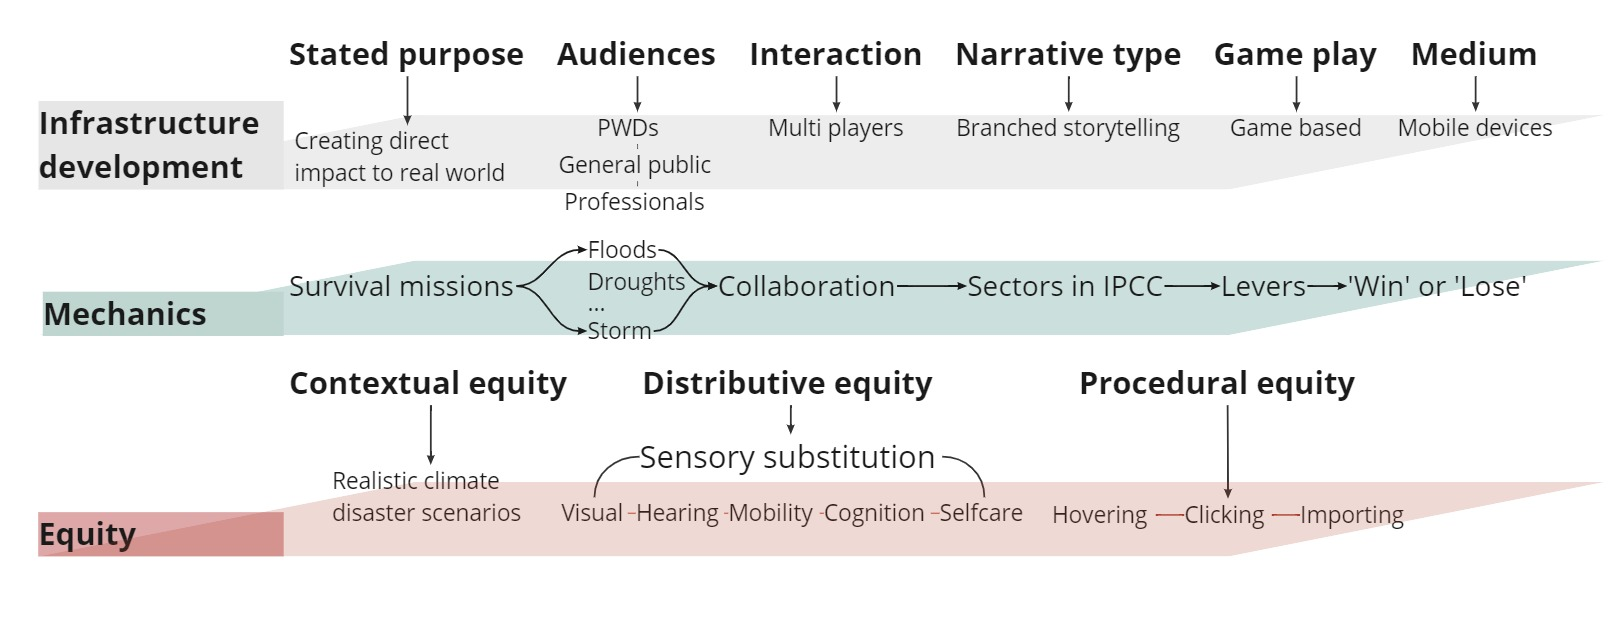
\includegraphics[width=0.95\textwidth]{Game2.jpg}
    \caption{Preliminary three layer framework for narrative game design: infrastructure, mechanics and equity.}
    \label{fig:game-framework}
\end{figure}

The \textit{infrastructure} layer covers the delivery format, narrative structure and audience: branched storytelling on an accessible digital medium, with persons with disabilities as primary participants and disability advocates as co-designers. This responds directly to the critical disability studies reading of disability as a product of environmental and institutional barriers \cite{oliver_1990_politics,stjernholm2025critical}: the research medium itself must not reproduce the ableist normalisation that institutional theory identifies in routine planning \cite{dimaggio_powell_1983_ironcage,brown2025massachusetts}.

The \textit{mechanics} layer turns climate adaptation challenges into scenario based missions structured around hazards such as floods, heatwaves and transport disruption, each with decision points connected to accessibility, communication and policy levers. This layer operationalises the capability approach \cite{sen_1999_development,ton2021agency,villeneuve2021pcep}: each decision point is built to surface the conversion factors that turn formal entitlements into actual functioning. Allowing participants to test alternative arrangements is also intended to disrupt the system justification dynamic identified in Phase 1 \cite{jost_2003_decade,Akike2025}, since presenting the existing arrangement as one of several options rather than as the default opens it to evaluation.

The \textit{equity} layer draws on McDermott, Mahanty and Schreckenberg's \cite{mcdermott2013examining} three-dimensional framework, originally developed for payments for ecosystem services. \textit{Distributive equity} concerns the allocation of benefits, costs and risks across actors; \textit{procedural equity} concerns the inclusiveness and transparency of the decision-making processes through which those allocations are made; \textit{contextual equity} concerns the pre-existing social, political and economic conditions—capabilities, power and access to information—that shape who can enter procedures and what outcomes are attainable. The three are interlocking: distributive outcomes are produced through procedures, and both are conditioned by context. In the game, contextual equity grounds the scenarios in real climate risks and the social conditions that shape adaptive choices \cite{eriksen2025rock,stein2022disability}; distributive equity concerns the allocation of adaptation resources such as accessible shelters, transport and communication systems \cite{gartrell2020cambodia,Harpur2025}, the lens through which the social dominance dynamics around vulnerability framing become visible \cite{sidanius_pratto_1999_socdom}; procedural equity covers DPO co-design and meaningful participation in the choices made within the game \cite{pertiwi2019dpo,villeneuve2017dpo,rahatiningtyas2025yogyakarta}.

Figure~\ref{fig:scenario-preview} illustrates an indicative visual design of the scenario.

\begin{figure}[H]
    \centering
    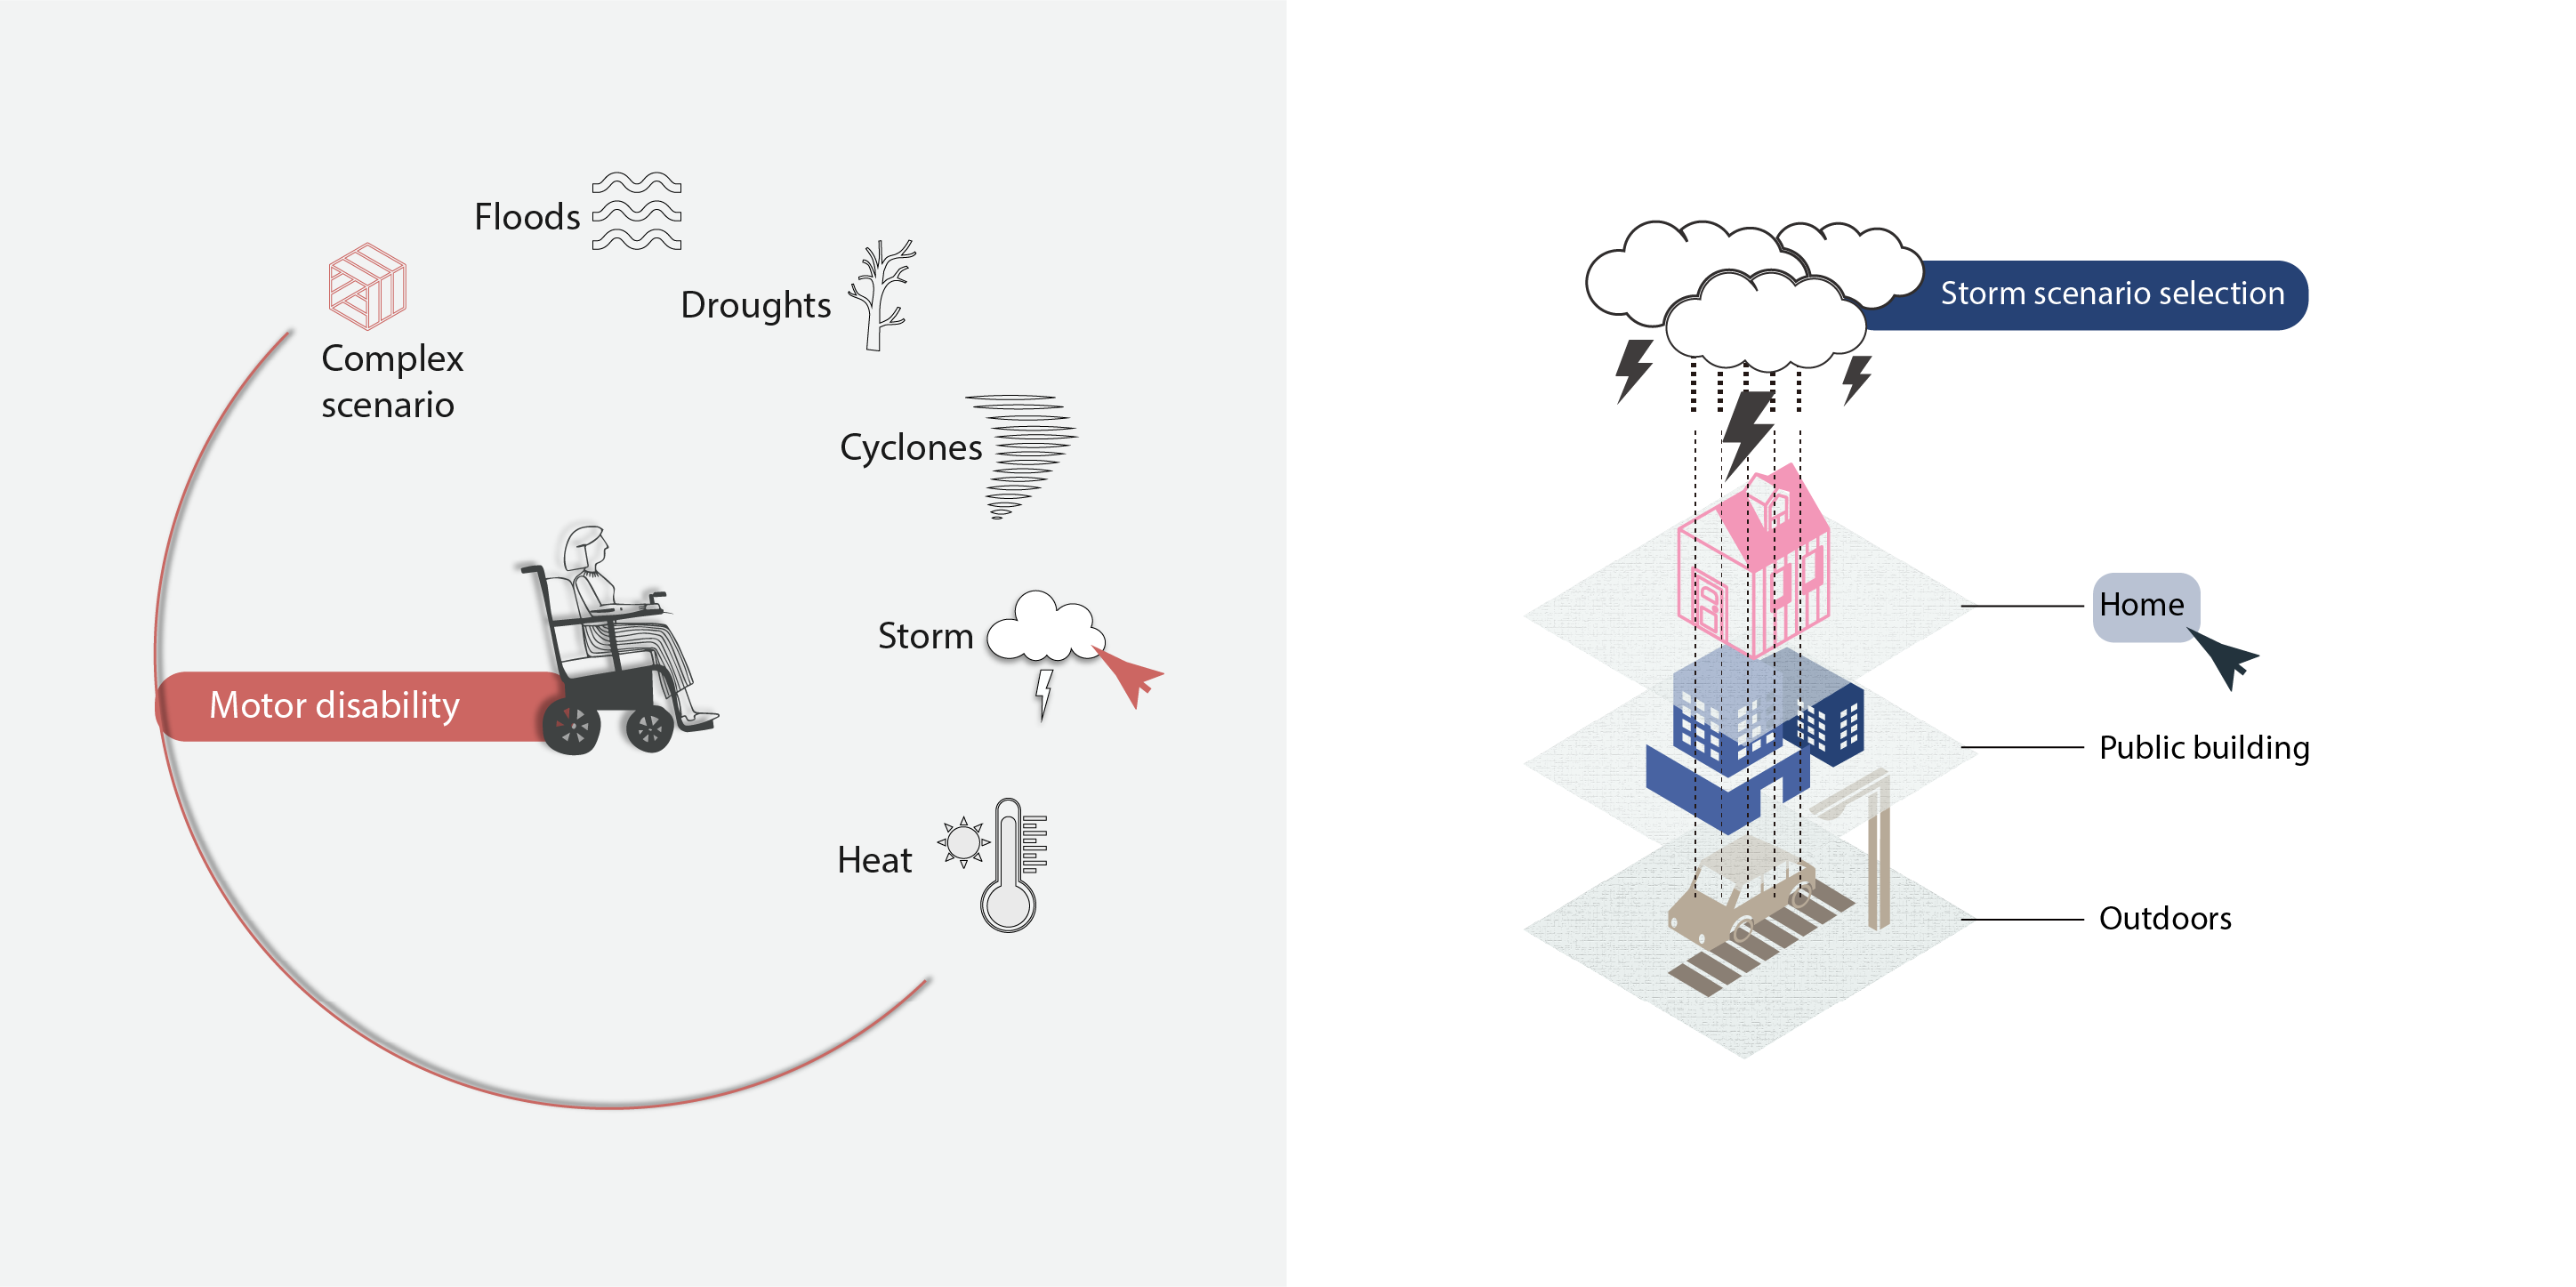
\includegraphics[width=0.95\textwidth]{Scenairo.png}
    \caption{Preview of a sample game scenario.}
    \label{fig:scenario-preview}
\end{figure}

\section{Participant focus and context}
The first round of the pilot will recruit people with mobility disabilities. Three reasons support this starting point. Climate-related hazards interact with mobility in particularly direct and well documented ways, flood evacuation, heatwave exposure in non-air-conditioned environments, transport disruption and the accessibility of emergency shelters, so the corpus provides a substantial evidence base against which scenarios can be calibrated \cite{villeneuve2021pcep,quaill2019queensland,brown2025massachusetts}. Accessibility requirements for engaging this group in screen based participatory research are well established and can be met without inventing new interface conventions, which is appropriate for a pilot that is testing the method rather than the technology. And DPO networks for mobility disability are comparatively well developed, supporting the DPO led recruitment route identified as essential in Phase 1 \cite{pertiwi2019dpo,villeneuve2017dpo}.

Disability is still not treated as a homogeneous category. The pilot will set the criteria under which the framework can be extended in subsequent rounds to sensory, cognitive, communication and self-care related access needs, in line with the scale and specificity tension identified in the literature \cite{craig2023twintrack,calgaro2021silent}. China remains the possible initial pilot context because of its accessibility and adaptation policy developments and its alignment with the researcher's intended impact pathway, though the framework is designed to be portable.

\section{Accessibility, ethics and DPO co-design}
Accessibility is a design requirement rather than a post hoc adjustment, and is specified in the first round for participants with mobility disabilities. The interface will be operable without fine motor control: full keyboard navigation, switch access compatibility and large interactive targets are baseline requirements, and any pointer based interaction will have a non-pointer equivalent. Decisions are made without time pressure to accommodate fatigue and variable response times, and sessions can be paused, resumed and saved. Where the pilot is conducted in person, the venue must meet step free access, accessible toilet provision and accessible transport routing; a remote option will run in parallel and is not treated as a fallback. Screen reader compatibility, alternative text and simplified language are retained as cross cutting requirements that benefit mobility-disabled participants with secondary access needs. Ethical risks are taken seriously: scenarios will avoid unnecessarily distressing content, consent procedures will be accessible, and participants can pause, skip or withdraw at any point. Recruitment and design will route through DPOs working with people with mobility disabilities, consistent with the DPO led participation pattern identified in Phase 1 \cite{pertiwi2019dpo,villeneuve2017dpo,rahatiningtyas2025yogyakarta}.

\section{Pilot evaluation and link to Phase 3}
The pilot will evaluate whether the game (i) is understandable and accessible, (ii) is perceived as relevant by participants and DPO partners, and (iii) generates data rich enough to feed downstream analysis. Three data types are expected: behavioural data on choices and decision pathways, narrative data on participant explanations and reflections, and usability and accessibility feedback. The behavioural and narrative data will be analysed in Phase 3 through Grounded Theory and, where the textual dataset is large enough, Topic Modelling, with the resulting concepts feeding the agent attributes, decision rules and policy levers of the Phase 4 agent based model.

\section{Summary}
This chapter has set out a preliminary narrative game framework rather than a finalised design. The framework operationalises the design criteria derived from Phase 1: decision level evidence under realistic policy options, DPO co-design at the centre, and disability group specificity preserved across participants. The full game specification, ethics approval and pilot recruitment will be developed in Year~2, after which Phase 3 will use the generated data to identify the behavioural concepts that anchor the agent based model in Phase 4.

\clearpage
\chapter{Future Research Plan (Phases 3 and 4): From Game Evidence to ABM Policy Simulation}
\vspace*{-1cm}

This chapter sketches the future research plan for Phases 3 and 4. Phase 3 will analyse the data generated by the narrative game in Chapter~5 using GT as the primary interpretive method and TM as a supplementary one. Phase 4 will translate the resulting concepts into the ABM that simulates how disability-inclusive climate adaptation policies perform under impairment-relevant heterogeneity. As with Chapter~5, the framework is preliminary: detailed analytical protocols, model specifications and validation strategies will be developed in Years~2 and~3.
\clearpage

\section{Phase 3: Grounded Theory and Topic Modelling}


Phase 3 analyses participants' choices, decision pathways, reflections and feedback from the narrative game pilot using two complementary qualitative-analytical traditions. GT generates theoretical categories from qualitative data, allowing behavioural evidence from the game to be coded into conceptual frameworks \cite{williams2019art,geertz2008thick}, though the categories it produces can be shaped by analyst assumptions. TM addresses this by applying probabilistic techniques from natural language processing to identify thematic patterns across large text sets \cite{Makuyana2023,grimmer2013text,jelodar2019latent}; pairing GT with TM reduces analyst bias \cite{debnath2020grounded,baumer2017comparing}, and the two methods recur as an analytical pair across the PhD, TM having already been used in Phase~1 to organise the literature \cite{debnath2020grounded}.

GT will be the primary method, beginning with open coding of concepts such as risk perception, institutional trust, accessibility barriers, informal support and policy acceptance, followed by axial coding to relate these concepts and selective coding to identify core themes. TM will be used as a supplementary lens where the textual dataset is large enough to support it, surfacing recurring patterns across participant responses without replacing the qualitative interpretation. The expected output is a set of disability-specific behavioural mechanisms that can be operationalised in Phase~4.


\section{Translating Phase 3 findings into ABM components}
The translation from qualitative findings to ABM components is the methodological bridge of the remaining work. Participant access needs become agent attributes (mobility, communication, information access, support availability); adaptive strategies observed in the game become agent decision rules, for example relying on informal networks when official systems are inaccessible, or staying in place when shelters are inaccessible; accessibility barriers become environmental and institutional constraints in the model environment; and policy perceptions become parameters that shape whether agents accept or reject policy options. Each translation step will be documented transparently, and sensitivity analysis in Phase 4 will test how robust the model is to the assumptions made.

\section{Phase 4: Agent-based modelling and policy simulation}

Phase 4 addresses a methodological challenge that runs across the PhD: policy evaluation in complex socio-behavioural systems requires both quantitative models that can simulate human-environment interactions at scale \cite{swart2004problem} and qualitative approaches that generate the contextual understanding which quantitative methods alone cannot produce \cite{moezzi2017using}. ABM is a computational approach suited to the complexity of social governance systems: where equation-based models struggle to represent heterogeneous, rule-governed behaviour, ABM simulates autonomous agents whose interactions generate aggregate outcomes \cite{macal2005tutorial,bonabeau1999swarm}, allowing the PhD to move from the diagnosis of exclusion mechanisms to the testing of policy scenarios.

Phase 4 will build the ABM to evaluate disability-inclusive climate adaptation policy scenarios. The behavioural categories generated in Phase~3 are translated into the model: agents represent persons with disabilities and, where relevant, institutional actors or service providers, defined by the attributes and decision rules derived in Phase~3 and parameterised by empirical results from the game data, so that they carry the heterogeneous adaptive behaviours, barrier experiences and institutional responses identified there. The environment includes climate hazards, infrastructure conditions, communication channels and policy levers. Policy scenarios will test alternative configurations of accessible communication, transport support, shelter provision, community-based support networks and participatory planning, spanning interventions such as mandatory accessibility requirements, participatory planning mandates and resource allocation mechanisms, with outcomes measured in terms of access to safety, resource uptake, policy compliance, unmet needs and equity across disability groups.

The model is exploratory rather than predictive: validation will rest on internal coherence with Phase~3 findings, the plausibility of simulated behaviour and stakeholder review where feasible, supported by sensitivity analysis on the key parameters. This is the PhD's main contribution to policy-relevant evidence: not another account of exclusion, but a simulation-based assessment of which governance interventions are most likely to generate inclusive outcomes under real-world social complexity.


\section{Ethical and methodological risks}
Five risks structure the ethical and methodological plan. Accessibility risk will be managed by iterative co-design with DPOs and by accessibility audits at each pilot stage. Emotional risk from emergency themed scenarios will be managed by trigger warnings, pacing controls and a clear withdrawal path. Data privacy risk will be managed through anonymisation, accessible consent procedures and explicit data management protocols. Overgeneralisation risk will be addressed by reporting sample limitations transparently and presenting the ABM as an exploratory rather than predictive tool. Translation risk, the danger that complex lived experience is flattened into model variables, will be addressed by documenting every translation step and by sensitivity analysis. The overarching commitment is reflexive: the PhD must not reproduce the exclusion it sets out to critique.

\clearpage
\chapter{Conclusion}
\vspace*{-1cm}

This report sets out the full four-year PhD work plan on disability-inclusive climate adaptation governance. Year~1 has been completed and is documented in this report as Phase~1; Years~2 to~4 are planned below. The plan's central argument is that disability is increasingly recognised in formal climate adaptation policy yet remains operationally thin, that this gap is reproduced through identifiable behavioural mechanisms rather than being a passive absence of evidence, and that the remaining phases of the PhD are designed to act on those mechanisms directly.

The chapters develop this argument incrementally. Chapter~1 frames the policy and lived-experience problems and the four-phase research design; Chapters~2 and~3 set out the conceptual ground and methodological framework. Chapter~4 documents the completed Phase~1 along three converging tracks. bibliometric analysis, BERTopic topic modelling and a qualitative synthesis of a 42-record core dataset, and identifies four behavioural patterns of exclusion (vulnerability framing, internalised acceptance of token inclusion, DPO led participation against weak partnership architecture, institutional normalisation) mapped to five social-science frameworks. Chapter~5 translates these findings into the Phase~2 narrative-game framework, with the first pilot round scoped to people with mobility disabilities. Chapter~6 outlines Phases~3 and~4: grounded theory and topic modelling analysis of the pilot data, and a disability-sensitive agent based model carrying disability heterogeneity and disaggregated outcomes through to policy projection.

Three pivotal implications follow. The gap is structural rather than accidental, so a method designed to act on the mechanisms reproducing it can reasonably be expected to address it; the empirical design is deliberately bounded, starting with mobility disability and extending to other access needs once the pilot has established the criteria for that extension; and the project's distinctive contribution is methodological as well as substantive, coupling narrative behavioural evidence to a disability-sensitive ABM in an architecture not currently present in the literature.

In summary, this report sets out a four-phase PhD that diagnoses the architectural gap in disability-inclusive climate adaptation governance, identifies the behavioural mechanisms that reproduce it, and proposes a methodological response combining a participatory narrative game, qualitative analysis and a disability-sensitive agent based model; the key milestones across the four years are shown in Figure~\ref{fig:phd_gantt}. The commitment running through all four phases is reflexive: the project must not reproduce the exclusion it sets out to critique.

\begin{figure}[H]
  \centering
  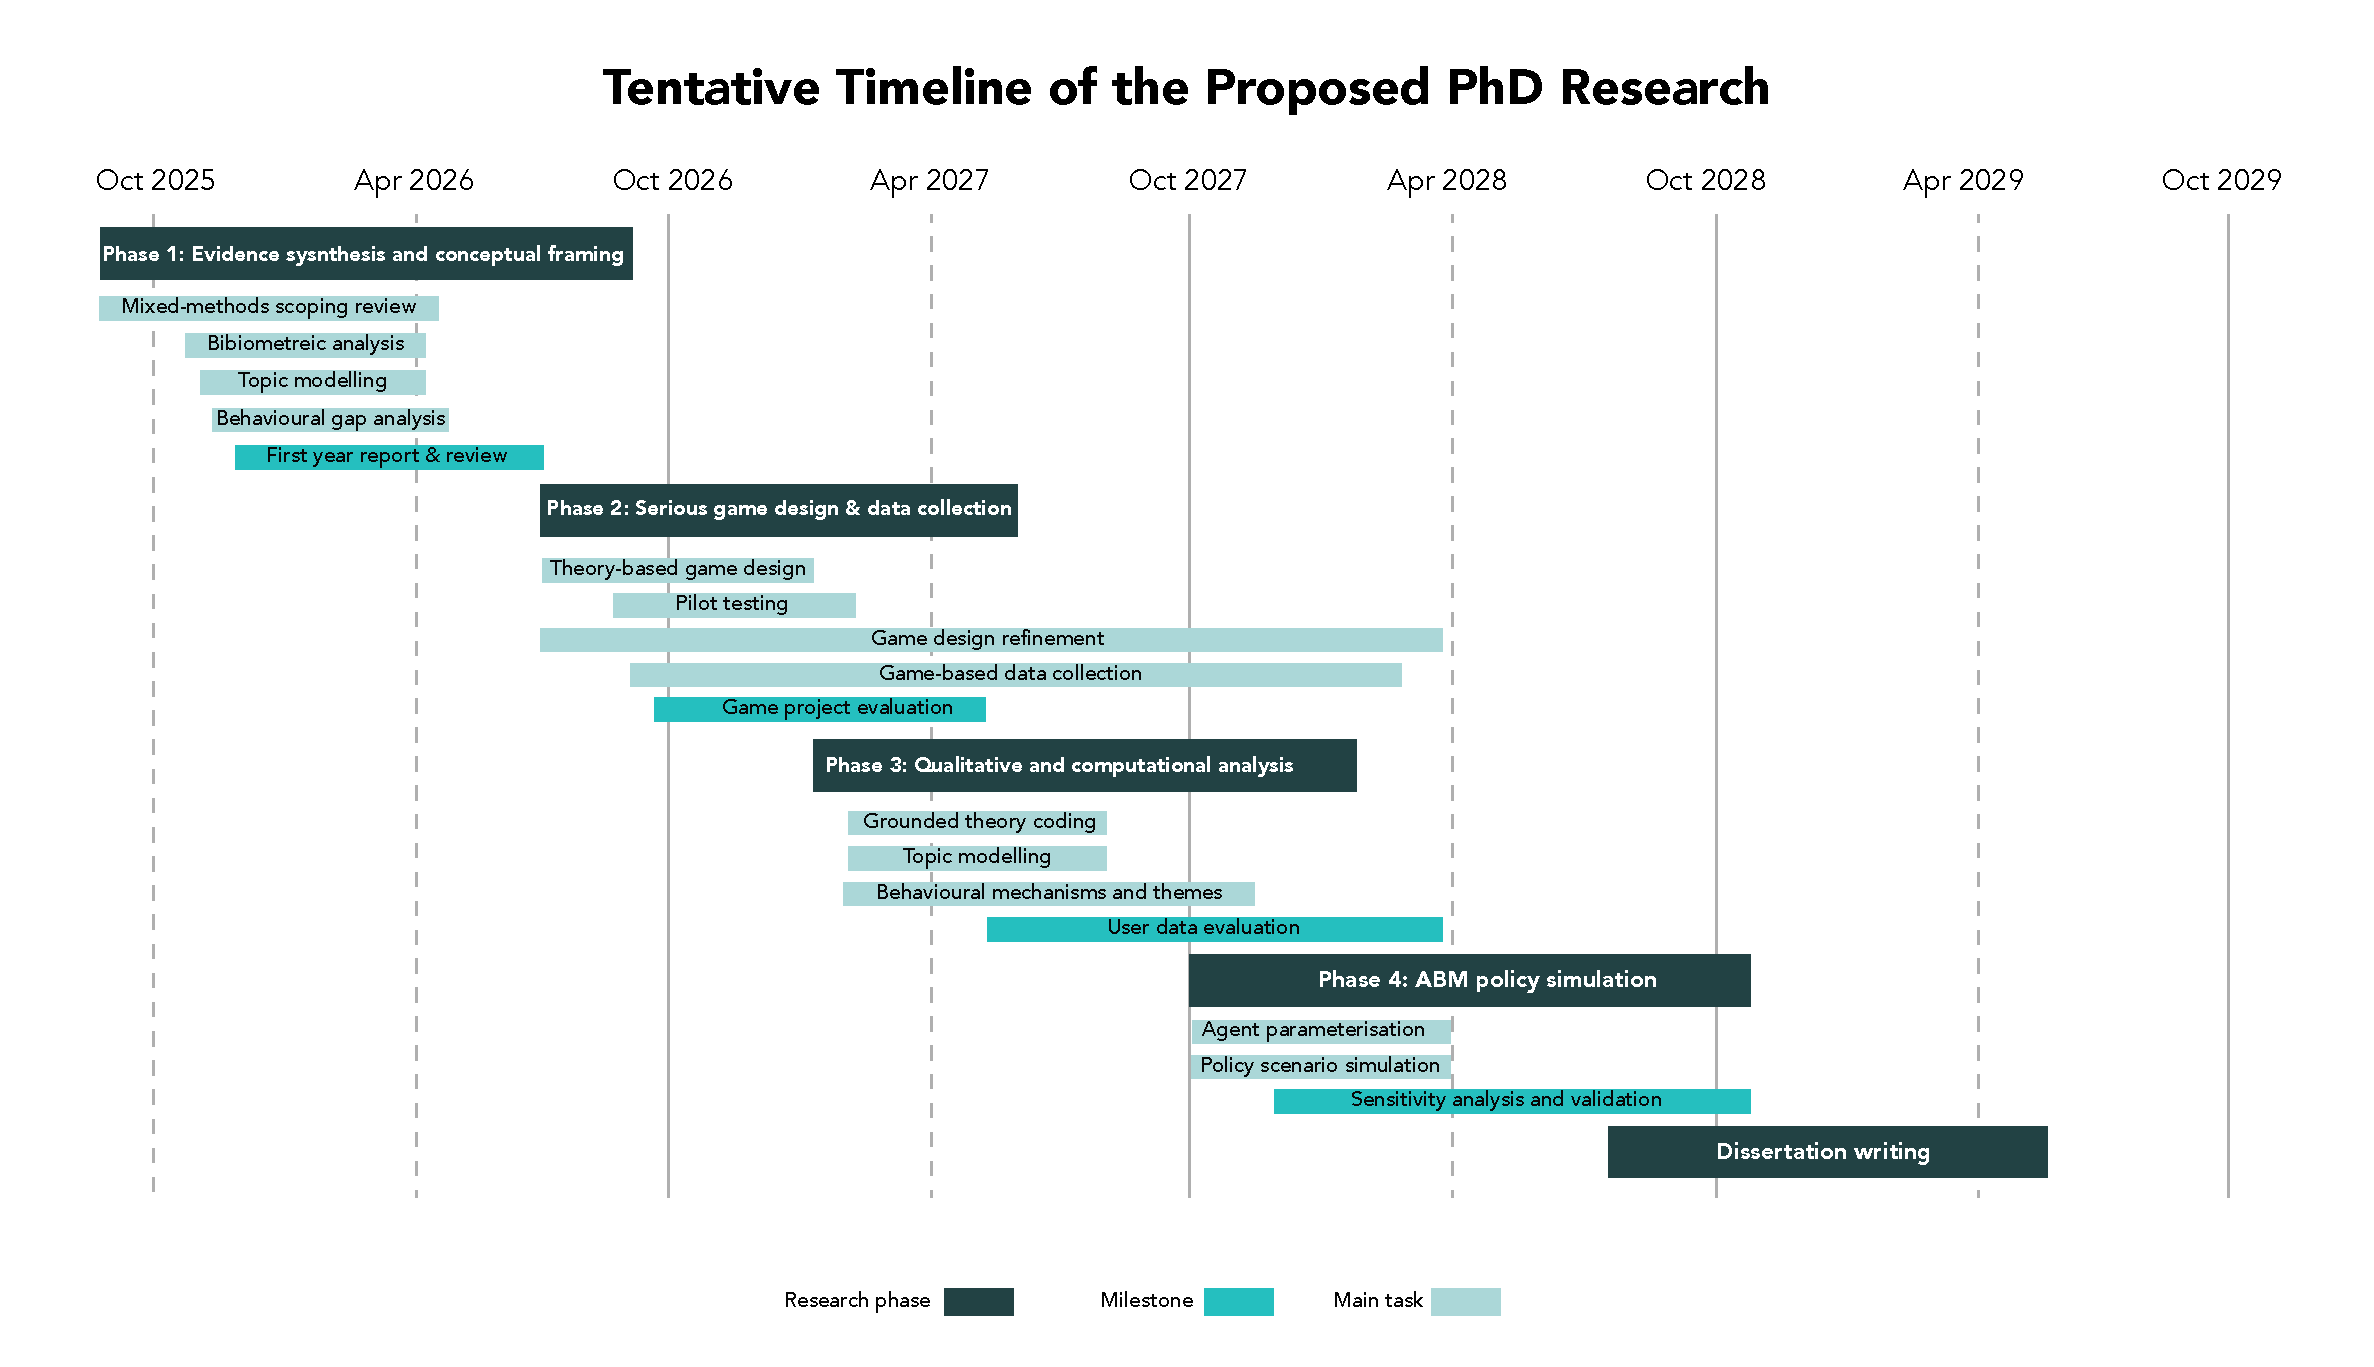
\includegraphics[width=\textwidth]{phd_gantt_timeline.pdf}
  \caption{Tentative Gantt chart of the proposed PhD research plan and key milestones.}
  \label{fig:phd_gantt}
\end{figure}
\clearpage



\clearpage
\phantomsection
\addcontentsline{toc}{section}{Appendix A: Search Keywords and Search String}

\noindent{\Large\bfseries Appendix A: Search Keywords and Search String}

\vspace{1em}

Only considered papers where the authors used one of the following common accessibility terms in the title, abstract, or author keywords:

\vspace{0.8em}


%\noindent\textbf{Complete search string:}

\begin{quote}
\small
\raggedright
(``climate change'' OR ``climate adaptation'' OR ``adaptation to climate change'' OR ``climate resilience'' OR ``disaster risk reduction'' OR ``climate risk'' OR ``climate governance'' OR ``climate policy'' OR ``climate justice'') AND (``disability'' OR ``people with disabilities'' OR ``persons with disabilities'' OR ``disabled people'' OR ``impairment'' OR ``functional limitation'' OR ``activity limitation'' OR ``participation restriction'' OR ``activities of daily living'' OR ``ADL'' OR ``social participation'' OR ``community participation'' OR ``social inclusion'' OR ``social exclusion'')
\end{quote}

% \subsection{Summary of Year 1 Progress}
% This first-year report has presented the development of the PhD project Evaluating Disability-Inclusive Climate Adaptation Policies through Narrative Gaming and Agent-Based Modelling. The project began from the aim of integrating serious narrative gaming, Grounded Theory, Topic Modelling and Agent-Based Modelling to evaluate and improve climate adaptation policies for persons with disabilities. During the first year, this broad aim has been refined through a deeper engagement with disability-inclusive climate governance literature and the development of a mixed-methods scoping review.

% The main progress in Year 1 has been the establishment of the conceptual and methodological foundation of the PhD. This includes the refinement of the research aim and questions, the development of a mixed-methods review design, the construction of review datasets, bibliometric and topic modelling analyses, and the initial identification of social-behavioural mechanisms of disability marginalisation in climate governance.
% \subsection{Contribution to the Overall PhD}
% The Year 1 review has played a central role in clarifying the direction of the PhD. It shows that existing literature has made important progress in recognising the disproportionate climate risks faced by persons with disabilities, but remains less developed in relation to agency, participation, behavioural evidence, implementation and policy evaluation.

% This finding strengthens the rationale for the next stages of the PhD. The serious narrative game is proposed as a participatory method for generating disability-specific behavioural and narrative data. Grounded Theory and Topic Modelling will be used to analyse these data, while Agent-Based Modelling will translate the findings into policy simulation. In this way, the PhD moves from literature-based diagnosis to empirical data generation and computational policy evaluation.
% \subsection{Next Steps}
% The immediate next steps are to finalise the Year 1 review paper, refine the conceptual framework, and develop the serious narrative game design in greater detail. This will include specifying game scenarios, accessibility requirements, data collection protocols and ethical considerations. The project will then move towards ethics preparation, pilot study design, participant recruitment planning and the identification of ABM variables.

% Overall, the first year has transformed the PhD from a broad proposal into a more coherent research pathway. The project now has a clearer thesis story: disability-inclusive climate adaptation requires not only policy recognition, but also participatory behavioural evidence and policy evaluation methods that can reflect the lived experiences, adaptive strategies and decision-making processes of persons with disabilities.

%\subsubsection{environmental justice to understand disabilities} Disabled populations are the largest marginalised group. This group consists of approximately 15 per cent of the global population. If care providers — parents, children and relatives caring for a disabled family member are accounted for, the percentage would be much higher. Almost everyone in their lifetime is likely to temporarily or permanently experience disability \cite{kosanic2022inclusive}.  Building disability resilience to climate change requires addressing complex uncertainties\cite{groulx2017role,swart2004problem}. This offers an opportunity to unite disability communities, social scientists, and data scientists in developing research that mitigates climate impacts on PWDs. A rights-based approach, aligned with the CRPD and the Sustainable Development Goals (SDGs)\cite{arstein2020introducing, kosanic2022inclusive}, should guide research\cite{arstein2020introducing}\cite{fuso2019connecting}: (1) Co-generating knowledge with disability leadership\cite{3}. (2) Prioritizing disability rights\cite{International_Disability_Alliance_2021, Pacific_Disability_Forum_2022}. (3)Ensuring knowledge is accessible by incorporating PWDs' lived experiences\cite{eriksen2021crdps}\cite{cohen1998climate}.  \subsection{Scenario Development} Uncertainties in social behaviour and climate change can be managed by interdisciplinary systems research in climate-related assessments. Combining quantitative methods with qualitative storylines to create alternative futures\cite{van2008new},\cite{wiebe2018scenario,carter2001developing,change2001climate}, is a novel approach. \subsubsection{Integrating Quantitative and Qualitative Methods for Modelling} Quantitative models simulate human-environment interactions\cite{swart2004problem}, while qualitative methods provide context by analyzing relationships between actions and outcomes\cite{moezzi2017using}. Agent-based Modelling (ABM) is a key quantitative paradigm for climate-related human-social interactions, simulating autonomous agents to reflect social behaviour and decision-making\cite{macal2005tutorial},\cite{bonabeau1999swarm}. Although precise, quantitative methods struggle with complex socio-ecological systems. Grounded Theory (GT) bridges this gap by generating theory, though it remains time-consuming and biased\cite{williams2019art,geertz2008thick}. Integrating Topic Modelling (TM) with GT reduces bias and enhances insights by identifying key themes in data\cite{debnath2020grounded}. TM, used in natural language processing, organizes vocabulary into probability distributions, with high-probability words forming “topics”\cite {grimmer2013text},\cite{jelodar2019latent}. ABM, GT and TM together will support robust, evidence-based policymaking across diverse future scenarios\cite{debnath2020grounded}\cite{baumer2017comparing}.



%\section{Data and Methods}
%This scoping review employed a sequential mixed-methods design comprising three analytical phases: bibliometric analysis, latent Dirichlet allocation (LDA) topic modelling, and thematic synthesis within a scoping review framework. The sequential structure was intentional. The first two phases were applied to a broad background review dataset to map the structural knowledge landscape at the intersection of disability and climate change, identifying dominant research framings and structural knowledge gaps. The third phase examined the nature and range of exclusionary patterns within a theoretically-focused core dataset. Social Dominance Theory and System Justification Theory were applied as analytical lenses during the synthesis phase to interpret identified patterns and illuminate their underlying behavioural mechanisms. The review was conducted in accordance with the Preferred Reporting Items for Systematic Reviews and Meta-Analyses extension for Scoping Reviews (PRISMA-ScR) guidelines, and the scoping review methodology followed the framework proposed by Arksey and O'Malley (2005) and refined by Levac et al. (2010).

%\subsection{Search strategy}
%The search keyword strategy was informed by the WHO International Classification of Functioning, Disability and Health (ICF), which conceptualises disability as the outcome of interactions between health conditions and contextual factors (both personal and environmental), rather than as a set of diagnostic categories. Applied to climate research, this biopsychosocial perspective directs attention to the contextual determinants of vulnerability and adaptive capacity, aligning with how disability is operationalised in climate adaptation scholarship\cite{gaskin2017factors}. A systematic search was conducted across three electronic databases — Web of Science, Scopus, and PubMed — covering publications from 2006 to 2025 in English. The year 2006 was selected as the starting point to coincide with the adoption of the United Nations Convention on the Rights of Persons with Disabilities (CRPD), which marked the formal international recognition of disability rights within governance frameworks. The search string combined climate-related terms with disability-related terms using Boolean operators: ("climate change" OR "climate adaptation" OR "adaptation to climate change" OR "climate resilience" OR "disaster risk reduction" OR "climate risk" OR "climate governance" OR "climate policy" OR "climate justice") AND (disab* OR "people with disabilities" OR "persons with disabilities" OR "disabled people" OR impairment OR "functional limitation" OR "activity limitation" OR "participation restriction*" OR "activities of daily living" OR ADL OR "social participation" OR "community participation" OR "social inclusion" OR "social exclusion").

%\subsection{Search slection} The search keywords were revised three times during the development of the search strategy. Terms related to vulnerability (e.g., "vulnerabl*") were tested during the exploratory phase but were not retained in the final search. Their inclusion substantially increased the number of retrieved records, primarily by capturing a wide range of general climate vulnerability studies in which disability was only marginally referenced or treated as one of many intersecting vulnerabilities. To preserve conceptual specificity and to enable an analysis of disability as a distinct social identity rather than a generic vulnerability category, these terms were excluded from the final search strategy. The inclusion of more disability-specific keywords (e.g., "blind", "deaf") was also considered but ultimately rejected, as narrowing the search to particular impairment categories risked introducing bias and misrepresenting the broader landscape of disability scholarship.

%The screening and selection process followed the PRISMA-ScR flow diagram (Figure 1). The initial search yielded 7,672 records, which were reduced to 4,299 after the removal of 2,477 duplicates. Title and abstract screening was conducted independently by two reviewers, with disagreements resolved through discussion. The screening process applied a sequential set of exclusion criteria to progressively refine the dataset, ultimately yielding two datasets serving distinct analytical purposes. The background review dataset (n=267) comprised all articles addressing the intersection of disability and climate change regardless of analytical orientation, and was used for bibliometric analysis and topic modelling. The core dataset (n=36) comprised empirical and analytical studies explicitly examining disability positioning or exclusion mechanisms within climate governance contexts, and was used for thematic synthesis within the scoping review framework.
%\begin{figure}[H]
    %\centering
    %\includegraphics[width=0.7\textwidth]{prisma_diagram.png}
   % \caption{PRISMA ScR Flow Diagram.}
    %\label{fig:enter-label}
%\end{figure}

%\subsection{Search criteria}
%We identified studies by searching the following 3 electronic databases: Web of Science, Scopus and PubMed. Only considered papers where the authors used one of the following common accessibility terms in the title, abstract, or authorkeywords: "climate change" OR "climate adaptation" OR "adaptation to climate change" OR "climate resilience" OR "disaster risk reduction" OR "climate risk" OR "climate governance" OR "climate policy" OR "climate justice" ) AND ( disab* OR "people with disabilities" OR "persons with disabilities" OR "disabled people" OR impairment* OR "functional limitation*" OR "activity limitation*" OR "participation restriction*" OR "activities of daily living" OR ADL OR "social participation" OR "community participation" OR "social inclusion" OR "social exclusion".
%We also searched for gray literature using the Google search engine and the websites of 4 organizations: PICC, UN agencies, NGO reports. Including resolutions, reports, documents and publications.




%\begin{itemize}
    %\item Source Distribution: The 205 articles were distributed across [X] journals, with a long tail of single-publication outlets indicating substantial dispersion. The most active venues were International Journal of Disaster Risk Reduction (n=12), Disaster Prevention and Management (n=5), International Journal of Disaster Risk Science (n=5), and Journal of Climate Change and Health (n=3). Disability-focused journals such as Disability and Society (n=3) and the African Disability Rights Yearbook (n=2) appeared less frequently than disaster and climate journals, suggesting that the topic has been engaged with predominantly from disaster risk and climate science perspectives rather than from within disability studies.
%\end{itemize}
%\begin{itemize}
    %\item Keyword Co-occurrence Analysis: A keyword co-occurrence analysis was conducted using VOSviewer, with a minimum threshold of three occurrences per keyword. After harmonising synonymous terms and removing generic bibliographic descriptors through a thesaurus file, 125 keywords were retained and organised into six clusters (Figure 3). The map shows three main thematic concentrations. The first centred on disability, persons with disabilities, vulnerability, disaster risk reduction, disaster management, resilience, inclusion, participation, and human rights, suggesting that disability is commonly framed through vulnerability, preparedness, and risk-management language. The second grouped climate change, climate adaptation, health impacts, public health, sustainable development, environmental justice, and natural disasters, indicating a climate-health and adaptation-oriented framing. The third included demographic and public-health terms such as children, adults, older people, women, men, epidemiology, temperature, and health risks, suggesting that disability is often treated as a population or vulnerability variable. The density visualisation showed high concentrations around climate change, disability, persons with disabilities, vulnerability, and disaster risk reduction. In contrast, terms related to policy, decision-making, participation, marginalisation, and disability inclusion appeared less central. This indicates a field-level gap: the literature is still more strongly organised around vulnerability, health impacts, and risk reduction than around governance, agency, participation, and exclusion.



%\begin{itemize}
   % \item Temporal Evolution of Concepts: The overlay visualisation, in which keyword colour reflects the average publication year of articles containing that term, revealed a clear temporal trajectory. Earlier literature (pre-2021) was dominated by epidemiological and emergency management framings, with demographic descriptors and vulnerability, preparedness, and emergency management appearing in older publications. More recent publications (2023–2025) were associated with climate justice, ableism, intersectionality, extreme weather events, and disaster prevention, suggesting an emerging but nascent shift toward rights-based and structural approaches. Governance and participation concepts, where present, also skewed toward more recent years, confirming that this dimension remains critically underdeveloped relative to the field's normative trajectory.
%\end{itemize}

%\subsection{Materials}
%The initial dataset in this paper is drawn from a study on the factors associated with environmental barriers of PWWS\cite{giraldo2019factors}. Additionally, the Climate-Economy Regional Agent-Based model and the OMOLAND-CA model can serve as a foundation to kickstart the project\cite{hailegiorgis2018}\cite{taberna2024navigating}. 
%\subsection{Framework of the Agent-based Model}
%This framework focuses on modelling the responses of PWDs to climate-related events, assessing how climate policies impact their survival and resilience through using ABM. This model simulates interactions between defined agents, including PWDs, policymakers, and key levers of the Intergovernmental Panel on Climate Change (IPCC) framework\cite{stocker2014summary}. Agents are characterized by static attributes such as disability level, and adaptive capacity for PWDs, and dynamic attributes include policy decisions and resource allocation for policymakers.

%The core element involves defining agent behaviours and designing spatial and social environments. Feedback loops capture social, policy, and environmental relationships.  Climate events and policies follow predefined rules, iteratively tested and calibrated with game data to ensure an accurate assessment of policy equity for PWDs. This model simulates non-linear decision-making, forming the game’s foundational logic.
%\subsection{System of the Serious Game}
%This serious game translates the ABM into an interactive platform combining narrative and simulation, building on three dimensions, outlined in Figure 2.
%\begin{figure}[H]
    %\centering
    %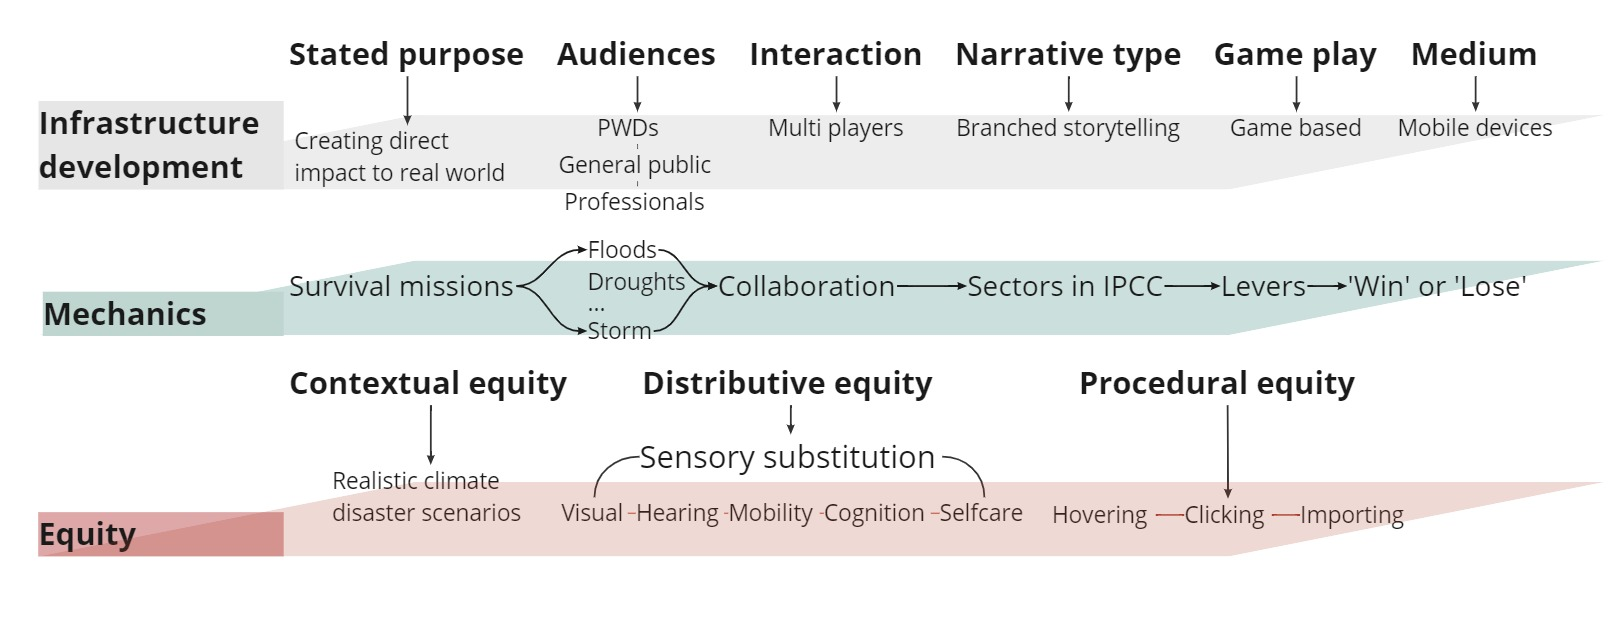
\includegraphics[width=1\linewidth]{Game2.jpg}
    %\caption{A three-layer framework diagram for game design}
    %\label{fig:enter-label}
%\end{figure}

%The foundation set is about infrastructure development. The game would address real-world challenges, target PWDs-centred multi-players, offer a branching disability categories narrative, etc. 

%The second dimension involves gameplay mechanics. Players with disabilities complete climate survival missions, following CRPD guidelines, and simulating events. Using levers mentioned in ABM (sectors like energy and health), success relies on selecting strategies. The Player Involvement Model"\cite{calleja2007revising} will be applied to enhance engagement and allow for continuous, disability-centered data collection.

%The third dimension integrates distributive, procedural, and contextual equity\cite{mcdermott2013examining}. Distributive equity adapts resources to the six core disability domains\cite{bickenbach2011world}. Such as using auditory cues for players with visual impairments, and incorporating music and voice input for feedback. Procedural equity promotes inclusive decision-making, while contextual equity reflects the climate environment. Tailored interactions like hovering, clicking, and importing enhance disability-centered experiences.

%\subsection{Nested Deep Narrative of the Game Analysis}
%Since the behaviour of people with disabilities (PWD) in response to climate change is underexplored, nested deep-narrative analysis starting with grounded theory (GT) allows theory to emerge directly from the data, ideal for discovering new behaviours and strategies. Topic modelling (TM) then quantifies these patterns, offering statistical validation. This approach captures both rich, real-world insights and data-driven patterns.
%\begin{itemize}
    %\item Qualitative Extraction - Grounded Theory: Starting with an open-ended question: 'How do PWD players use policy levers in the game?' allowing theory to emerge from the data. Analysis proceeds in three steps: open coding groups player behaviors into concepts, like “resource scarcity” representing key actions and strategies. axial coding links these into themes, and selective coding identifies core categories that explain behaviours and shape the game narrative. Data collection continues until theoretical saturation is reached.
%\end{itemize}

%\begin{itemize}
   % \item Quantitative Purifying - Topic Modelling:  LDA topic modelling validates and builds on GT patterns by identifying hidden topics in-game behaviours. This unsupervised machine-learning technique reveals strategies or decision-making frameworks through term analysis, and discrepancies between qualitative and quantitative findings refine the theory.
    
%When no new insights emerge, findings are synthesized into a theory explaining key phenomena, such as how PWD players develop adaptive strategies during climate stress. GT evolves iteratively through ongoing analysis and testing.
%\end{itemize}
%\begin{itemize}
   % \item ABM Calibration: The Agent-Based Model(ABM) is refined to align with the theory from the game, mapping GT concepts to agent behaviours.
    %Variables like policy complexity and fairness, along with agent attributes such as trust in institutions, are updated to influence policy acceptance. The model is fine-tuned using GT insights and quantitative data to simulate behaviours and forecast public opinion on policy proposals, providing data-driven recommendations.
%\end{itemize}
%\section{Expected Outcomes}
%This proposal develops a framework combining game design, Grounded Theory, and Agent-Based Modeling to simulate and predict public acceptance and effectiveness of climate resilience policies for PWDs. The goal is to support inclusive, equitable policies that empower vulnerable communities to adapt to climate change, ensuring no one is left behind. Figure 3 previews a partial scenario selection from the game.

%\section{Timeline of PhD}


\printbibliography


\end{document}

\bibliographystyle{alpha}   #选择引用样式
\bibliography{Reference}          #参考文献存放目录ref.bib文件
\end{document}



You can simply upload a \verb|.bib| file containing your BibTeX entries, created with a tool such as JabRef. You can then cite entries from it, like this: \cite{greenwade93}. Just remember to specify a bibliography style, as well as the filename of the \verb|.bib|. You can find a \href{https://www.overleaf.com/help/97-how-to-include-a-bibliography-using-bibtex}{video tutorial here} to learn more about BibTeX.

If you have an \href{https://www.overleaf.com/user/subscription/plans}{upgraded account}, you can also import your Mendeley or Zotero library directly as a \verb|.bib| file, via the upload menu in the file-tree.
Use the figure environment and the caption command to add a number and a caption to your figure. See the code for Figure \ref{fig:frog} in this section for an example.

Note that your figure will automatically be placed in the most appropriate place for it, given the surrounding text and taking into account other figures or tables that may be close by. You can find out more about adding images to your documents in this help article on \href{https://www.overleaf.com/learn/how-to/Including_images_on_Overleaf}{including images on Overleaf}.





Use the table and tabular environments for basic tables --- see Table~\ref{tab:widgets}, for example. For more information, please see this help article on \href{https://www.overleaf.com/learn/latex/tables}{tables}. 

\subsection{Good luck!}


\bibliographystyle{alpha}
\bibliography{sample}

\end{document}

